% bristolthesis template.tex file
% Best not to fiddle with this much/at all or things might break
% This needs to line up with the contents of bristolthesis.cls and vice versa
%
%
%
%
%

\documentclass[11pt,twoside]{bristolthesis}

%% Packages - these are those which i used for my thesis so might not be specific to yours
\usepackage{graphicx,latexsym}
\usepackage{amsmath}
\usepackage{amssymb}
\usepackage{amsthm}
\usepackage{longtable}
\usepackage{booktabs}
\usepackage{setspace}
\usepackage{siunitx}
% \usepackage{chemarr} %% Useful for one reaction arrow, useless if you're not a chem major
\usepackage[hyphens]{url}
\usepackage{hyperref}
\usepackage{lmodern}
\usepackage{float}
\floatplacement{figure}{H}
\usepackage{rotating}
% \usepackage{times} % other fonts are available like times, bookman, charter, palatino
\usepackage{lscape}
\newcommand{\blandscape}{\begin{landscape}}
\newcommand{\elandscape}{\end{landscape}}

%% Paramaters for global document
\hypersetup{colorlinks = false}
\renewcommand{\UrlBreaks}{\do\/\do\a\do\b\do\c\do\d\do\e\do\f\do\g\do\h\do\i\do\j\do\k\do\l\do\m\do\n\do\o\do\p\do\q\do\r\do\s\do\t\do\u\do\v\do\w\do\x\do\y\do\z\do\A\do\B\do\C\do\D\do\E\do\F\do\G\do\H\do\I\do\J\do\K\do\L\do\M\do\N\do\O\do\P\do\Q\do\R\do\S\do\T\do\U\do\V\do\W\do\X\do\Y\do\Z\do\0\do\1\do\2\do\3\do\4\do\5\do\6\do\7\do\8\do\9\do\%\do\.\do\-}
\renewcommand{\chapterautorefname}{Chapter}
\usepackage{times} % other fonts are available like times, bookman, charter, palatino
\usepackage{caption}

% Use ref for internal links
\renewcommand{\hyperref}[2][???]{\autoref{#1}}
\def\chapterautorefname{Chapter}
\def\sectionautorefname{Section}
\def\subsectionautorefname{Subsection}
\usepackage{caption}
\captionsetup{width=5in}

% Syntax highlighting #22
%%%

%%% YAML header functions
\title{The association between adiposity and platelet function: implications for cardiovascular disease}
\author{Lucy Goudswaard}
\date{March 2022}
\university{University of Bristol}
\faculty{Life Sciences}
\school{Physiology, Pharmacology and Neuroscience / Population Health Sciences}
\group{Bristol Platelet Group / Team Timpson}
\wordcount{}
\degree{PhD}
\logo{figure/index/UoBcrest.pdf}
%%%


%%% The document formatting
\makeatletter
\def\maxwidth{ %
  \ifdim\Gin@nat@width>\linewidth
    \linewidth
  \else
    \Gin@nat@width
  \fi
}
\makeatother

\renewcommand{\contentsname}{Table of Contents}

\setlength{\parskip}{14truept}

  \setlength{\parskip}{\baselineskip}
  \usepackage[parfill]{parskip}

\providecommand{\tightlist}{%
  \setlength{\itemsep}{0pt}\setlength{\parskip}{0pt}}

\Acknowledgements{
First of all, I would like to say a huge thanks to my supervisors Professor Ingeborg Hers and Professor Nicholas Timpson for their guidance and advice throughout my PhD. I have felt supported when I have needed it, but also feel like I have been given the independence and academic freedom, which I will take forward into my career. It goes without saying that this work would not have been possible without the British Heart Foundation Integrative Cardiovascular Science PhD programme, along with the funding I received from the University of Bristol alumni.

Thank you to all the members of Bristol Platelet Group and Team Timpson who have been so encouraging, supportive and willing to help me, especially in the early stages of my PhD. Although interrupted by the pandemic, I enjoyed all the pub trips and socials that I attended when they were allowed!

I would also like to thank my family and friends for their support throughout my PhD. To my flat mates of 3.5 years, Tessa and Josie, thanks for the support and motivation to keep going, especially in each lockdown when all we saw was each other. And lastly, thank you to Harry. Whether it be sending gifts for abstracts being accepted, printing out my first publication into a booklet or just offering words of encouragement, he has been a rock through it all!
}

\Declaration{
I declare that the work in this dissertation was carried out in accordance with the requirements of the University's Regulations and Code of Practice for Research Degree Programmes and that it has not been submitted for any other academic award. Except where indicated by specific reference in the text, the work is the candidate's own work. Work done in collaboration with, or with the assistance of, others, is indicated as such. Any views expressed in the dissertation are those of the author.

\bigskip
\bigskip
\bigskip
\bigskip
\bigskip

Signed

\bigskip
\bigskip
\bigskip
\bigskip
\bigskip

Dated
}

\Abstract{
Variation in adiposity is associated with thrombotic outcomes, but mechanisms leading from this exposure to disease are unclear. The overall aims were to assess the effect of adiposity on platelet function (key cells involved in thrombosis) and identify potential mechanisms.

Data from INTERVAL (a UK study of blood donors), COPTIC (Bristol-based cardiac surgery cohort) and DiRECT (Diabetes REmission Clinical Trial in Glasgow/Newcastle) were used. The effect of body mass index (BMI) on platelet traits measured by Sysmex XN-1000 was assessed in INTERVAL (N=33,388) using Mendelian randomization (MR). The association between platelet traits and platelet function was explored using linear regression in COPTIC (N=655). Bariatric patient (BMI \textgreater40kg/m2) platelet function was also compared with controls (BMI 18.5-25kg/m2). MR evidence in INTERVAL suggested that higher BMI raises immature platelet count (IPC - newly produced platelets). Results from COPTIC indicated that greater IPC is associated with greater platelet aggregation. Validation work in a specifically designed study of bariatric patients and healthy weight controls is ongoing.

To identify the involvement of the circulating proteome in adiposity-related platelet changes, the causal effect of BMI on \textgreater3600 proteins measured by SomaLogic was estimated using MR (N=2,737). To complement this, the effect of weight loss on the serum proteome was examined using linear regression in the DiRECT cohort (N=265). Adiposity had a substantial effect on the plasma proteome: higher BMI raised levels of leptin and fumarylacetoacetase while reducing sex hormone binding-globulin levels.

These analyses suggest that higher BMI raises immature platelet count (newly produced platelets), which are pro-thrombotic. The proteomic analyses from different study designs point towards potential proteins which may influence platelet production and function which require further investigation. Future analyses would include developing approaches to compare protein profiles across cohorts. Overall, these analyses provide novel mechanistic insight into how higher BMI causes disease.
}

\Abbreviations{
```\{r abbreviations, echo=FALSE\}
library(readxl)
library(tidyr)
library(kableExtra)
abbreviations \textless- read\_xlsx(``figure/Abbreviations/Abbreviations.xlsx'')
abbreviations \textless- abbreviations{[}order(abbreviations\$Abbreviation),{]}

abbreviations \%\textgreater\% kable(caption = ``Full list of abbreviations'', booktabs = TRUE) \%\textgreater\%
kable\_classic\_2(full\_width = F) \%\textgreater\%
kable\_styling(full\_width = TRUE) \%\textgreater\%
column\_spec(1, width = ``3cm'')
```
}

	\usepackage{tikz} \usepackage{booktabs} \usepackage{longtable} \usepackage{siunitx} \pagestyle{plain}
	\usepackage{booktabs}
 \usepackage{longtable}
 \usepackage{array}
 \usepackage{multirow}
 \usepackage{wrapfig}
 \usepackage{float}
 \usepackage{colortbl}
 \usepackage{pdflscape}
 \usepackage{tabu}
 \usepackage{threeparttable}
 \usepackage{threeparttablex}
 \usepackage[normalem]{ulem}
 \usepackage{makecell}
 \usepackage{xcolor}

\newlength{\cslhangindent}
\setlength{\cslhangindent}{1.5em}
\newlength{\csllabelwidth}
\setlength{\csllabelwidth}{3em}
\newenvironment{CSLReferences}[2] % #1 hanging-ident, #2 entry spacing
 {% don't indent paragraphs
  \setlength{\parindent}{0pt}
  % turn on hanging indent if param 1 is 1
  \ifodd #1 \everypar{\setlength{\hangindent}{\cslhangindent}}\ignorespaces\fi
  % set entry spacing
  \ifnum #2 > 0
  \setlength{\parskip}{#2\baselineskip}
  \fi
 }%
 {}
\usepackage{calc}
\newcommand{\CSLBlock}[1]{#1\hfill\break}
\newcommand{\CSLLeftMargin}[1]{\parbox[t]{\csllabelwidth}{#1}}
\newcommand{\CSLRightInline}[1]{\parbox[t]{\linewidth - \csllabelwidth}{#1}\break}
\newcommand{\CSLIndent}[1]{\hspace{\cslhangindent}#1}

\DeclareUnicodeCharacter{03B2}{\ensuremath{\beta}} 
\DeclareUnicodeCharacter{0392}{\ensuremath{\beta}}          % β% β
\DeclareUnicodeCharacter{03B1}{\ensuremath{\alpha}}
\DeclareUnicodeCharacter{2265}{\ensuremath{\geq}}
\DeclareUnicodeCharacter{2264}{\ensuremath{\leq}}
\DeclareUnicodeCharacter{2008}{\ensuremath{\space}}
\DeclareUnicodeCharacter{223C}{\ensuremath{\tilde}}


%%% Main document
\spacing{1}
\begin{document}
  \maketitle



\frontmatter % this stuff will be roman-numbered
\pagestyle{empty} % this removes page numbers from the frontmatter
  \begin{abstract}
    Variation in adiposity is associated with thrombotic outcomes, but mechanisms leading from this exposure to disease are unclear. The overall aims were to assess the effect of adiposity on platelet function (key cells involved in thrombosis) and identify potential mechanisms.

    Data from INTERVAL (a UK study of blood donors), COPTIC (Bristol-based cardiac surgery cohort) and DiRECT (Diabetes REmission Clinical Trial in Glasgow/Newcastle) were used. The effect of body mass index (BMI) on platelet traits measured by Sysmex XN-1000 was assessed in INTERVAL (N=33,388) using Mendelian randomization (MR). The association between platelet traits and platelet function was explored using linear regression in COPTIC (N=655). Bariatric patient (BMI \textgreater40kg/m2) platelet function was also compared with controls (BMI 18.5-25kg/m2). MR evidence in INTERVAL suggested that higher BMI raises immature platelet count (IPC - newly produced platelets). Results from COPTIC indicated that greater IPC is associated with greater platelet aggregation. Validation work in a specifically designed study of bariatric patients and healthy weight controls is ongoing.

    To identify the involvement of the circulating proteome in adiposity-related platelet changes, the causal effect of BMI on \textgreater3600 proteins measured by SomaLogic was estimated using MR (N=2,737). To complement this, the effect of weight loss on the serum proteome was examined using linear regression in the DiRECT cohort (N=265). Adiposity had a substantial effect on the plasma proteome: higher BMI raised levels of leptin and fumarylacetoacetase while reducing sex hormone binding-globulin levels.

    These analyses suggest that higher BMI raises immature platelet count (newly produced platelets), which are pro-thrombotic. The proteomic analyses from different study designs point towards potential proteins which may influence platelet production and function which require further investigation. Future analyses would include developing approaches to compare protein profiles across cohorts. Overall, these analyses provide novel mechanistic insight into how higher BMI causes disease.
  \end{abstract}
  \begin{acknowledgements}
    First of all, I would like to say a huge thanks to my supervisors Professor Ingeborg Hers and Professor Nicholas Timpson for their guidance and advice throughout my PhD. I have felt supported when I have needed it, but also feel like I have been given the independence and academic freedom, which I will take forward into my career. It goes without saying that this work would not have been possible without the British Heart Foundation Integrative Cardiovascular Science PhD programme, along with the funding I received from the University of Bristol alumni.

    Thank you to all the members of Bristol Platelet Group and Team Timpson who have been so encouraging, supportive and willing to help me, especially in the early stages of my PhD. Although interrupted by the pandemic, I enjoyed all the pub trips and socials that I attended when they were allowed!

    I would also like to thank my family and friends for their support throughout my PhD. To my flat mates of 3.5 years, Tessa and Josie, thanks for the support and motivation to keep going, especially in each lockdown when all we saw was each other. And lastly, thank you to Harry. Whether it be sending gifts for abstracts being accepted, printing out my first publication into a booklet or just offering words of encouragement, he has been a rock through it all!
  \end{acknowledgements}
  \begin{declaration}
    I declare that the work in this dissertation was carried out in accordance with the requirements of the University's Regulations and Code of Practice for Research Degree Programmes and that it has not been submitted for any other academic award. Except where indicated by specific reference in the text, the work is the candidate's own work. Work done in collaboration with, or with the assistance of, others, is indicated as such. Any views expressed in the dissertation are those of the author.

    \bigskip
    \bigskip
    \bigskip
    \bigskip
    \bigskip

    Signed

    \bigskip
    \bigskip
    \bigskip
    \bigskip
    \bigskip

    Dated
  \end{declaration}
  \hypersetup{linkcolor=black}
  \setcounter{tocdepth}{3}
  \tableofcontents
  \listoftables
  \listoffigures

\spacing{1.5}
\mainmatter % here the regular arabic numbering starts
\pagestyle{plain}
\hypertarget{preface}{%
\chapter*{Preface}\label{preface}}
\addcontentsline{toc}{chapter}{Preface}

\hypertarget{introduction}{%
\chapter*{Introduction}\label{introduction}}
\addcontentsline{toc}{chapter}{Introduction}

\hypertarget{format}{%
\section{Format}\label{format}}

This chapter will provide some background information to put the thesis into context. It will provide information on obesity, in particular its prevalence and implications for cardiovascular disease. Possible mechanisms of disease will be introduced, such as the involvement of platelets. At the end of this chapter, the aims of the thesis will be introduced.

\hypertarget{background}{%
\section{Background}\label{background}}

\hypertarget{obesity-on-the-rise}{%
\subsection{Obesity on the rise}\label{obesity-on-the-rise}}

Obesity, defined as a body mass index (BMI) of greater than 30kg/m\textsuperscript{2}, has tripled worldwide since 1975. It is currently estimated that 40\% of adults in the United States and 26\% of adults in the United Kingdom have obesity.\textsuperscript{1} As of 2016, the number of individuals globally with obesity surpassed 650 million.\textsuperscript{2} The average BMI of the UK adult population is \textasciitilde27kg/m\textsuperscript{2},\textsuperscript{3} which is in the `overweight' category (between 25 and 30 kg/m\textsuperscript{2}). Overweight is also more common than `normal-weight' in many other higher-income countries,\textsuperscript{4} and prevalence of overweight is increasing in lower-income countries.\textsuperscript{5}

BMI is generally used as a proxy for adiposity as there are high correlations between BMI and objective measures of fat mass measured by dual-energy X-ray absorptiometry (DXA),\textsuperscript{6} such as total fat mass index and regional fat mass indices. Due to the specialised equipment needed for fat mass measures, BMI is often much more widely available within cohort studies and trials.

\hypertarget{obesity-is-a-modifiable-risk-factor-for-cardiovascular-disease}{%
\subsection{Obesity is a modifiable risk factor for cardiovascular disease}\label{obesity-is-a-modifiable-risk-factor-for-cardiovascular-disease}}

Adiposity is a risk factor for certain non-communicable diseases. Such diseases include Type 2 Diabetes mellitus (T2D), musculoskeletal diseases, certain types of cancer and cardiovascular disease.\textsuperscript{7--10} Collectively, treatment for obesity-related diseases is costly for health services.\textsuperscript{11,12} Cardiovascular disease is one of the leading causes of death. Cardiovascular disease is a general term for diseases affecting the heart or circulatory system and can be subcategorised further into diseases such as thrombotic disorders including coronary heart disease (CHD) and stroke. Obesity is associated with an increased risk of such cardiovascular events.\textsuperscript{8}

\hypertarget{mendelian-randomisation-can-be-used-to-explore-causality}{%
\subsection{Mendelian randomisation can be used to explore causality}\label{mendelian-randomisation-can-be-used-to-explore-causality}}

Mendelian randomisation is a technique which uses the random assortment of alleles to estimate the causal association between a modifiable risk factor (such as BMI) and disease outcomes. It can be likened to a natural randomised control trial (RCT) {[}FIG{]}. Associations between BMI and disease have been shown through use of prospective observational studies,\textsuperscript{8} but more recently, through use of Mendelian randomisation studies.\textsuperscript{13--15} These studies have provided evidence for a causal relationship between adiposity and ischaemic heart disease (IHD),\textsuperscript{13} coronary heart disease (CHD), T2D\textsuperscript{14} and types of cancer including pancreatic cancer.\textsuperscript{15} Studies have also found that weight loss improves cardiovascular risk factors {[}\textsuperscript{16}; other refs{]}. Despite the evidence for a causal association between adiposity and cardiovascular disease, mechanisms of obesity-related disease remain unclear.

\hypertarget{mechanisms-of-obesity-related-cardiovascular-disease}{%
\subsection{Mechanisms of obesity-related cardiovascular disease}\label{mechanisms-of-obesity-related-cardiovascular-disease}}

Obesity is caused by an increase in fat deposition and generally occurs when energy intake exceeds energy expenditure. There are two types of fat: white adipose tissue (WAT) and brown adipose tissue (BAT). WAT secretes proteins and peptides which have pro-inflammatory effects.\textsuperscript{17,18} Due to these adipose tissue effects, obesity results in a state of chronic low-grade inflammation,\textsuperscript{19} with an increase in adipose tumour necrosis factor-alpha (TNF-alpha) and interleukin-6 (IL-6).\textsuperscript{18} Efforts have been made to understand how adiposity causes cardiovascular disease, with suggestion that inflammation, increased production of reactive oxygen species and endothelial dysfunction contribute to increased cardiovascular risk.\textsuperscript{17, add other refs}

\hypertarget{plasma-markers-of-obesity}{%
\subsection{Plasma markers of obesity}\label{plasma-markers-of-obesity}}

Studies which have explored the molecular footprint of adiposity have tended to focus on the lipidome, such as cholesterol and triglycerides in lipoprotein subtypes, inlcuding low-density lipoproteins (LDL), very-low-density lipoproteins (VLDL) and high-density lipoproteins (HDL),\textsuperscript{20,21} where a higher BMI is associated with an increase in LDLs and a decrease in large HDLs. This has been expored in a causal framework.

As the majority of druggable targets are proteins, it is also valuable to explore the effects of BMI on circulating plasma proteins. It is estimated that 25\% of proteins in the human proteome circulate in the blood,\textsuperscript{22} including enzymes, protein kinases and transport proteins. Therefore, focusing on effects of adiposity on the circulating proteome may allow for the development of or repurposing of therapeutic interventions to reduce obesity-related disease. Previous studies that have explored the effect of adiposity on circulating proteins have used hypothesis driven approaches.\textsuperscript{23} Attempts to evaluate the effect of BMI on the general proteome have been performed using observational analyses.\textsuperscript{24} Recent technologies have been developed which allow protein detection in unprecedented scope and detail, for example the SOMAscan by SomaLogic,\textsuperscript{25} which can detect over 3,500 unique proteins. Although identifying alterations of individual proteins may provide therapeutic opportunities, assessing the overall protein profile of adiposity may provide more of a mechanistic insight into how adiposity causes disease.

\hypertarget{platelets-are-key-cells-involved-in-thrombosis}{%
\subsection{Platelets are key cells involved in thrombosis}\label{platelets-are-key-cells-involved-in-thrombosis}}

Platelets are enucleate blood cells that are involved in the cessation of bleeding, but can cause thrombosis when activated pathologically.
Antiplatelet drugs used to prevent reocurrence of MI.
BMI is linked to increased rates of thrombosis, therefore it is likely that platelets become hyperactive. There is conflicting literature surrounding this and cohorts to explore these effects are limited.

\hypertarget{importance-of-interdisciplinary-methods}{%
\subsection{Importance of interdisciplinary methods}\label{importance-of-interdisciplinary-methods}}

Each approach has biases and problems, which means we need to be careful \ldots.
A combination of laboratory experiments, clinical studies and epidemiology (including Mendelian randomization and RCTs) in order to investigate mechanisms of disease.

\hypertarget{thesis-aims-and-objectives}{%
\subsection{Thesis aims and objectives}\label{thesis-aims-and-objectives}}

The aims of the thesis are indicated below, with a schematic of the multi-step pathway which this thesis aims to explore (Figure \ref{fig:Thesis-schematic}).
\begin{enumerate}
\def\labelenumi{\arabic{enumi})}
\tightlist
\item
\item
\item
\item
\end{enumerate}
\begin{figure}
\includegraphics{figure/Intro_background/Thesis_graphic_overview_without_chapters} \caption[Schematic of the multi-step pathway addressed in the thesis]{Schematic of the multi-step pathway addressed in the thesis}\label{fig:Thesis-schematic}
\end{figure}
\hypertarget{thesis-structure}{%
\subsection{Thesis structure}\label{thesis-structure}}

There will be xx results chapters in this thesis.
1)
2)
3)
4)

\hypertarget{publications-from-the-phd-in-preparation-or-published}{%
\subsection{Publications from the PhD (in preparation or published)}\label{publications-from-the-phd-in-preparation-or-published}}

\textbf{Goudswaard L. J.}, Bell J. A., Hughes D. A., Corbin L. J., Walter K., Davey Smith G., Soranzo N., Danesh J., Di Angelantonio E., Ouwehand W. H., Watkins N. A., Roberts D. J., Butterworth A. S., Hers I., Timpson N. J. Effects of adiposity on the human plasma proteome: Observational and Mendelian randomisation estimates (2021) Int J Obes \url{https://doi.org/10.1038/s41366-021-00896-1}

\textbf{Goudswaard L. J.}, Harrison S., Van De Klee D., Chaturvedi N., Lawlor D. A., Davey Smith G., Hughes A.D., Howe L. D. Blood pressure variability and night-time dipping assessed by 24-hour ambulatory monitoring: Cross-sectional association with cardiac structure in adolescents. (2021) PLOS ONE 16(6): e0253196. \url{https://doi.org/10.1371/journal.pone.0253196}

\textbf{Goudswaard L. J.}, Corbin L. J., Burley K. L., Mumford A., Akbari P., Soranzo N., Butterworth A. S., Watkins N. A., Pournaras D. J., Harris J., Timpson N. J., Hers I. Higher body mass index raises immature platelet count: evidence from Mendelian randomization analyses. (2021) medRxiv. \url{doi:10.1101/2021.05.19.2125744325}.

Liu, H., Jackson, M. L., \textbf{Goudswaard, L. J.}, Moore S. F., Hutchinson J. L, Hers I. Sphingosine-1-phosphate modulates PAR1-mediated human platelet activation in a concentration-dependent biphasic manner. (2021) Sci Rep 11, 15308. \url{https://doi.org/10.1038/s41598-021-94052-4}

Sledz, K. M., Moore, S. F., Vijayaragavan, V., Mallah, S., \textbf{Goudswaard, L. J.}, Williams, C. M., Hunter, R. W. \& Hers, I. Redundant role of ASK1-mediated p38MAPK activation in human platelet function. (2020) Cellular Signalling. 68, 11 p., 109528. \url{doi:10.1016/j.cellsig.2020.109528}

\hypertarget{presentations-from-the-phd}{%
\subsection{Presentations from the PhD}\label{presentations-from-the-phd}}

\textbf{Platelet Society meeting}, 2018, Cambridge, UK. Title: Do the chemokines MDC and TARC contribute to obesity related platelet hyperactivity and cardiovascular disease? (Oral presentation).

\textbf{IEU Scientific Advisory Board meeting}, 2020, Bristol, UK. Title: Effect of adiposity on the human plasma proteome: a Mendelian randomisation study using individual level data (Poster).

\textbf{International Genetic Epidemiological Society meeting}, 2020, Virtual conference. Title: Effects of body mass index on the human proteome: a Mendelian randomization study using individual level data (Selected for short talk as one of the top ranked posters).

\textbf{International Society of Thrombosis and Haemostasis meeting}, 2020, Virtual conference. Title: Effects of body mass index on the human plasma proteome -- potential drivers of obesity-related cardiovascular disease? (Poster).

\textbf{Platelet society meeting}, 2021, Virtual conference. Title: Altered platelet proteome, enhanced basal platelet procoagulant activity, and increased platelet-leukocyte interactions in patients with Covid-19. (Oral presentation)

\textbf{Platelet society meeting}, 2021, Virtual conference. Title: Estimating the causal association between body mass index and platelet properties: evidence for a positive association with immature platelet count (Poster)

\textbf{British Heart Foundation PhD Student Conference}, 2021, Virtual conference. Title: Estimating the association of body mass index and platelet properties: an observational and Mendelian randomization study (Poster)

\textbf{International Society of Thrombosis and Haemostasis meeting}, 2021, Virtual conference. Title: Altered platelet proteome and platelet-leukocyte interactions in patients with COVID-19 (Oral presentation and Travel Award, presented by Prof Hers)

\textbf{International Society of Thrombosis and Haemostasis meeting}, 2021, Virtual conference. Title: Estimating the causal association between body mass index and platelet properties: evidence for a positive association with immature platelet count (Oral presentation and Travel Award)

\textbf{World Congress of Epidemiology}, 2021, Virtual conference. Title: Effects of adiposity on the human proteome: Mendelian randomization study using individual-level data (Oral presentation)

\textbf{International Genetic Epidemiology Society}, 2021, Virtual conference. Title: Combining Mendelian randomization and randomized control trial study designs to determine effects of adiposity on the plasma proteome (Oral presentation)

\hypertarget{background-1}{%
\chapter*{Background}\label{background-1}}
\addcontentsline{toc}{chapter}{Background}

\hypertarget{section}{%
\section{}\label{section}}

\hypertarget{higher-body-mass-index-raises-immature-platelet-count-evidence-from-mendelian-randomization-analyses}{%
\chapter{Higher body mass index raises immature platelet count: evidence from Mendelian randomization analyses}\label{higher-body-mass-index-raises-immature-platelet-count-evidence-from-mendelian-randomization-analyses}}

This work is under review at xxxxxxxxx and is on the preprint server MedRXiV.\textsuperscript{26} I performed all analyses, created all figures and tables and wrote the manuscript.

\hypertarget{background-2}{%
\section{Background}\label{background-2}}

Obesity (body mass index ≥ 30 kg/m\textsuperscript{2}) has nearly tripled worldwide in the last 45 years.\textsuperscript{1} This is a major health concern as a higher body mass index (BMI) is an important risk factor for various noncommunicable disorders, including cardiovascular disease.\textsuperscript{27} Clinical studies and genetic association studies have identified BMI as an independent risk factor for thrombotic disorders, including coronary heart disease and stroke 4-6.\textsuperscript{13,14,28}

Platelets are blood cells which are essential for the cessation of bleeding upon injury to a blood vessel and are involved in thrombosis and progression of cardiovascular disease.\textsuperscript{29} When pathologically activated, platelets can aggregate to form thrombi thereby occluding arteries and triggering a myocardial infarction or stroke.\textsuperscript{29} Platelet hyperactivity can be an indicator of those who may be at an increased risk of thrombosis.\textsuperscript{30} There is evidence that people with a higher BMI have hyperactive platelets,\textsuperscript{31,32} which could explain why a higher BMI is linked to an increase in thrombosis. Mechanisms of platelet hyperactivity are unclear, but it is possible that changes in platelet numbers, size and immaturity may play a role. Furthermore, an alteration in circulating metabolites or proteins induced by obesity could modulate the activation of platelets.\textsuperscript{33}

Platelet function can be directly assessed by various methods; these methods commonly include platelet aggregation experiments and/or using antibodies to detect platelet receptors that are expressed upon activation. One of the limitations of measuring platelet function directly is that these techniques are not widely available or readily standardized. Haematology analyzers are more commonly used to provide full blood counts, providing detailed readouts of platelet characteristics. Some of these characteristics have been reported to be indirect measures of platelet function.\textsuperscript{34} For example, an increase in mean platelet volume (MPV) has been reported to be predictive of vascular mortality and ischaemic heart disease.\textsuperscript{35} Another commonly measured platelet characteristic is the number of platelets in circulation (platelet count, PLT). An increase in platelet count has been reported to be associated with platelet hyperactivity\textsuperscript{34} and there is evidence that higher platelet count is associated with ischaemic stroke.\textsuperscript{36}

Sysmex haematology analyzers are able to provide additional platelet characteristics, such as immature platelet fraction (IPF) and immature platelet count (IPC).\textsuperscript{37} Immature platelets (also known as reticulated platelets) are the youngest platelets in circulation and are detected based on having a greater forward scatter (FSC, an indicator of their size) and a greater side fluorescence (SFL, an indicator of their mRNA content).\textsuperscript{38} Higher levels of immature platelets are indicative of enhanced platelet production\textsuperscript{39} and these platelets are believed to be more prothrombotic than older circulating platelets, with more dense granule release and increased P-selectin expression.\textsuperscript{38--40} Higher immature platelet count is associated with adverse cardiovascular outcomes in patients with coronary artery disease\textsuperscript{38} and reduced effectiveness of antiplatelet therapies,\textsuperscript{40,41} suggesting that hyperactive immature platelets may contribute to adverse vascular events. Immature platelets have also been suggested to be less responsive to antiplatelet therapies such as prasugrel in acute coronary syndrome patients.\textsuperscript{40}

As these platelet characteristics provide potential information about platelet hyperactivity and given the increased thrombotic risk seen with adiposity, it is important to assess how adiposity affects platelet properties. Previous studies with modest samples sizes have implemented observational epidemiological methods to explore the effect of BMI on PLT, plateletcrit (PCT) and MPV. There is conflicting observational evidence regarding an association between BMI and PLT,\textsuperscript{42,43} with some studies suggesting a positive association between BMI and MPV\textsuperscript{44} and other studies reporting no such association.\textsuperscript{45} Furthermore, as there is evidence that immature platelet production is increased in patients with metabolic syndrome and type II diabetes,\textsuperscript{46,47} it is therefore important to explore whether BMI may be an independent predictor of this trait. It is currently unknown whether the influence of BMI on platelet properties and function are causal and independent of confounding effects.

In this study, we used data from the INTERVAL prospective cohort (N=33388) to explore the association between BMI and platelet traits. We combined observational and Mendelian randomization (MR) approaches to test the hypothesis that higher BMI leads to changes in platelet characteristics. Although observational studies can demonstrate associations between BMI and platelet characteristics, they cannot determine direct causality. To address the latter, we therefore employed MR, using a genetic risk score derived from single nucleotide polymorphisms (SNPs) associated with higher BMI (Figure \ref{fig:Linear-reg-MR}). This allowed estimation of the causal effect of BMI on platelet traits, reducing the effect of confounding factors that are inherent to observational studies. To assess functional implications of BMI-platelet associations, a follow-up analysis was designed to explore the associations between platelet characteristics and whole blood aggregation in a cohort of cardiac surgery patients.
\begin{figure}
\includegraphics{figure/BMI_platelets/obsvMRexample} \caption[Schematic of linear regression and Mendelian randomization analyses]{Schematic of linear regression and Mendelian randomization analyses. Linear regression assesses the association between BMI (exposure) and platelet traits (outcome), with adjustment for potential confounders. Under the assumptions of Mendelian randomization (MR), the genetic risk score (GRS) for body mass index (BMI) does not associate with confounding variables, and if there is a causal association, the GRS should only associate with platelet outcomes through its association with body mass index.}\label{fig:Linear-reg-MR}
\end{figure}
\hypertarget{methods}{%
\section{Methods}\label{methods}}

\hypertarget{study-population}{%
\subsection{Study population}\label{study-population}}

INTERVAL is a prospective cohort study that initially aimed to test the safety of reducing the time interval between donation of whole blood in 50 000 participants {[}\textsuperscript{48}. Participants were over the age of 18 years, able to provide informed consent and free from a history of major disease. Participants were recruited between June 11th, 2012 and June 15th, 2014 from 25 National Health Service Blood and Transplant (NHSBT) centres across England. They filled out online questionnaires including self-reported height and weight, smoking status and alcohol consumption. Blood samples were also taken at baseline (before randomization within the study) where full blood counts were obtained. The study was approved by Cambridge East Research Ethics Committee. Permission for data access was provided by the Data Access Committee. Data contains sensitive content and requires permission to use therefore cannot be made publicly available. Access to data needs to be approved by the INTERVAL team www.intervalstudy.org.uk/more-information.

The present study was conducted on up to 33 388 European ancestry participants living in the United Kingdom. These were the participants who had genetic data, had basic phenotype data and full blood count measures (Figure \ref{fig:INTERVAL-STROBE}). Participants were mostly of European descent.
\begin{figure}
\includegraphics[width=0.8\linewidth,height=0.8\textheight]{figure/BMI_platelets/STROBE_diagram} \caption{A STROBE diagram outlining participants included in the INTERVAL study (N=33388).}\label{fig:INTERVAL-STROBE}
\end{figure}
\hypertarget{measurement-of-bmi-and-covariables}{%
\subsection{Measurement of BMI and covariables}\label{measurement-of-bmi-and-covariables}}

Participants self-reported their weight and height using online questionnaires. BMI was derived from their weight in kilograms by the square of their height in metres (kg/m\textsuperscript{2}). BMI was rank normal transformed (rntransform() function from ``moosefun'' package \url{https://github.com/hughesevoanth/moosefun/}). Available covariables used in the analysis were age, sex, smoking status (in three categories of never, previous and current) and alcohol consumption (in four categories of rarely, less than once a week, 1-2 times a week and 3-5 times a week or most days). These covariables were chosen due to their plausible associations with both BMI and cardiovascular health,\textsuperscript{27} therefore it is important to adjust for these variables in the observational estimates.

\hypertarget{measurement-of-platelet-traits}{%
\subsection{Measurement of platelet traits}\label{measurement-of-platelet-traits}}

Blood was taken by venipuncture into 3mL EDTA tubes. Platelet parameters were measured using the Sysmex XN-1000 instrument.\textsuperscript{49} This analyzer provides information on cell counts by using a combination of fluorescence (PLT-F) and impedance (I) flow cytometry. The PLT-F channel used a Fluorocell fluorescent dye (oxazine), whereas the impedance method uses electrical resistance to detect platelets. Platelet indices included in the current study, along with the raw units, are provided in Table \ref{tab:Platelet-traits}. These measurements were pre-adjusted for technical covariates such as time between venipuncture and blood count, as well as instrument drift, seasonal and weekly variation.\textsuperscript{49} Adjustment was performed with cyclic, thin-plate and P-splines in a generalized additive model (GAM).\textsuperscript{50} Resulting platelet trait values along with their units of measurement are reported in Table \ref{tab:Platelet-traits}. These data were rank normal transformed to normalize the distribution of each trait. Therefore, each platelet index is measured in normalized standard deviation (SD) units.
\begin{landscape}\begin{table}

\caption[Platelet traits measured by Sysmex XN-1000]{\label{tab:Platelet-traits}Platelet traits measured by Sysmex XN-1000}
\centering
\begin{tabu} to \linewidth {>{\raggedright}X>{\raggedright\arraybackslash}p{4cm}>{\raggedright\arraybackslash}p{6cm}>{\raggedright}X>{\raggedright}X}
\toprule
Short name & Full name & Derivation of platelet trait & Units & Mean (SD)\\
\midrule
P-LCR & Platelet large cell ratio & (platelet number with volume>12 fL)/(platelet number of ordinary volume)  x 100 & \% & 36.9 (7.7)\\
H-IPF & High fluorescence immature platelet fraction & (high fluorescence immature platelet number)/(platelet count)  x 100 & \% & 1.3 (1.0)\\
PLT (F) & Platelet count (PLT-F channel) & Total number of platelets per litre & 109/L & 255 (57)\\
PLT (I) & Platelet count (impedance channel) & Total number of platelets per litre & 109/L & 250 (55)\\
PCT & Plateletcrit & Volume percentage of blood occupied by platelets & \% & 0.28 (0.06)\\
\addlinespace
PDW & Platelet distribution width & Standard deviation of platelet volume distribution, estimated as width at 20\% modal height of platelet volume histogram & fL & 14.0 (1.8)\\
IPC & Immature platelet count & Immature platelet count & 109/L & 10.1 (5.0)\\
IPF & Immature platelet fraction & (Immature platelet number)/(platelet count)   x 100 & \% & 4.2 (2.5)\\
MPV & Mean platelet volume & Mean platelet volume & fL & 11.1 (1.0)\\
SFL & Side fluorescence & Side fluorescence measures the nucleic acid (mRNA) content of the platelet & RFUs & 80.3 (5.0)\\
\addlinespace
FSC & Forward scatter & Forward scatter is a measure of the size of the platelet & RFUs & 53.0 (6.4)\\
SSC & Side scatter & Side scatter is a measure of the granularity of the platelet & RFUs & 37.9 (2.9)\\
\bottomrule
\end{tabu}
\end{table}
\end{landscape}
\hypertarget{genetic-data-and-the-association-of-the-genetic-risk-score-grs-with-bmi}{%
\subsection{Genetic data and the association of the genetic risk score (GRS) with BMI}\label{genetic-data-and-the-association-of-the-genetic-risk-score-grs-with-bmi}}

The genotyping of INTERVAL participants was performed using the Affymetrix GeneTitan® Multi-Channel (MC) Instrument. Quality control (QC) was performed as previously described.\textsuperscript{49} Imputation was implemented using a combined 1000 Genomes phase-3-UK + 10K reference panel using the Practical Byzantine Fault Tolerance (PBFT) algorithm.\textsuperscript{49} A genetic instrument for BMI was created by using 654 genetic variants available of the 656 variants which were independently associated with BMI (P\textless5x10-8) in a recent meta-analysis of GWAS of around 700,000 individuals of European descent.\textsuperscript{51} Of these individuals, 450,000 were from UK Biobank and 250,000 were from the Genetic Investigation of Anthropometric Traits (GIANT) consortium. The weighted GRS was made using PLINK 2.0.\textsuperscript{52} The effect alleles and beta coefficients were extracted from the source GWAS. The weighted score was calculated by multiplying the dosage of each effect alleles by its effect estimate, summing these and dividing by the number of SNPs (654). The GRS therefore reflects the average per-SNP effect on BMI per individual.

\hypertarget{statistical-analysis}{%
\subsection{Statistical analysis}\label{statistical-analysis}}

Analyses were performed using R version 3.4.2.\textsuperscript{53} To visualize correlation between outcome platelet variables, a correlation matrix was made using the pairwise Pearson correlation coefficients of the rank normal transformed data. A dendrogram was also created to show the hierarchical relationship between platelet traits (\url{https://github.com/hughesevoanth/iPVs}), where the height at which variables are joined is set at (1 -- Pearson correlation coefficient (r)). To explore observational associations between BMI and platelet traits, linear regression models were used (lm() function from ``stats'' package). Two regression models were used: firstly, adjusting for age and sex and secondly, additionally adjusting for smoking and alcohol consumption as ordinal variables. The results of the regression reflect the change in platelet traits (in normalized SD units) per normalized SD higher BMI (4.7 kg/m\textsuperscript{2}). Only participants with all covariables were included in the linear regression models. The associations between potential covariables with both BMI and platelet traits were also explored using linear regression.

To understand properties of the GRS for BMI, the association between the GRS with both BMI and covariables were explored. The MR analysis was performed by using a two-stage least squares (2SLS) regression model (using systemfit() function from ``systemfit'' package).\textsuperscript{54} The MR causal estimates reflect the change in platelet traits (in SD units) per SD increase in BMI. A Wu-Hausman test was performed to test for endogeneity between observational and MR estimates. Exact beta coefficients, confidence intervals and P values are provided throughout and guide strength of association.

\hypertarget{follow-up-analysis-to-explore-the-association-between-immature-platelets-and-aggregation}{%
\subsection{Follow-up analysis to explore the association between immature platelets and aggregation}\label{follow-up-analysis-to-explore-the-association-between-immature-platelets-and-aggregation}}

Motivated by findings from the primary analyses described above, additional observational analyses were conducted using data from the COagulation and Platelet laboratory Testing in Cardiac Surgery (COPTIC) study. The COPTIC study was an observational, single centre cohort study of adults undergoing cardiac surgery at the Bristol Heart Institute with primary objective of examining the relationship between coagulation laboratory parameters and bleeding outcomes after surgery in 2,541 participants.\textsuperscript{55} This study was approved by the UK NHS Research Ethics Committee (09/H0104/53).

\hypertarget{coptic-study-variables}{%
\subsection{COPTIC study variables}\label{coptic-study-variables}}

Age and sex were reported at baseline. Height and weight were obtained from medical notes. BMI was derived from weight and height (kg/m\textsuperscript{2}). Smoking was reported as a categorical variable (0=never smoker, 1=ex-smoker for \textgreater{} 5 years, 2=ex-smoker for 1-5 years, 3=ex-smoker for 30 days-1 year, 4=current smoker). Platelet variables (PLT, MPV, IPF, IPC) were measured using the Sysmex XE-2100 Automated Haematology System (Oxford, UK). Blood samples were taken pre-operatively into 3.2\% sodium citrate vacutainers (BD Biosciences, Milton Keynes, UK). Platelet aggregation was measured using Multiplate multiple electrode aggregometry (MEA) (Roche, Rotkreuz, Switzerland), which detects change in electrical impedance when platelets aggregate on metal electrodes. Aggregation was determined by the area under the curve (AUC) in response to platelet agonists including adrenaline (100 mg/mL), thrombin receptor activator peptide 6 test (TRAP-test), ADP-test and arachidonic acid (ASPI-test). Use of a combination of agonists therefore reflects activation of platelets via different pathways: adrenaline acts at the α2 adrenergic receptor, TRAP-6 acts at the protease-activated receptor-1 (PAR-1), ADP acts at the P2Y12 receptor and arachidonic acid at the Thromboxane A2 (TxA2) receptor.

\hypertarget{coptic-statistical-analysis}{%
\subsection{COPTIC statistical analysis}\label{coptic-statistical-analysis}}

The COPTIC dataset in the current analysis included 2,518 participants (23 out of 2,541 participants did not consent for future research). For the current study, only those who were not on antiplatelet therapies (prasugrel, clopidogrel or aspirin) were included (N=655). Extreme outliers that were ± 5 SDs from the mean were removed, and exposures and outcomes were rank normal transformed. Linear regression was used to explore the association between immature platelet count and aggregation, adjusting for age, sex and smoking status.

\hypertarget{results}{%
\section{Results}\label{results}}

\hypertarget{interval-participant-characteristics}{%
\subsection{INTERVAL participant characteristics}\label{interval-participant-characteristics}}

Of INTERVAL participants included in the current study (N=33,388), 50.2 \% were female. The mean age was 45.3 years (SD of 14.2 years, Table \ref{tab:INT-participants-platelets}). The mean BMI was 26.4 kg/m2 (SD of 4.7 kg/m2). The majority of participants were never smokers (58.9 \%), with 33.3\% and 7.8 \% reported as previous and current smokers, respectively. Nearly a third (32.7 \%) of participants reported drinking alcohol at least three times a week.
\begin{table}

\caption{\label{tab:INT-participants-platelets}Characteristics of included INTERVAL participants}
\centering
\begin{tabu} to \linewidth {>{\raggedright\arraybackslash}p{8cm}>{\raggedright}X>{\raggedleft}X}
\toprule
Variable & Mean (SD) or \% & N\\
\midrule
Age & 45.3 (14.2) & 33388\\
Sex &  & 33388\\
\hspace{1em}Male & 49.8\% & \\
\hspace{1em}Female & 50.2\% & \\
Weight (kg) & 78.2 (16.0) & 33455\\
\addlinespace
Height (cm) & 171.8 (9.6) & 33388\\
Body mass index (kg/m2) & 26.4 (4.7) & 33388\\
Smoking frequency &  & 32867\\
\hspace{1em}Never & 58.9\% & \\
\hspace{1em}Previous & 33.3\% & \\
\addlinespace
\hspace{1em}Current & 7.8\% & \\
Alcohol intake frequency &  & 29538\\
\hspace{1em}Rarely & 12.5\% & \\
\hspace{1em}Less than once a week & 17.1\% & \\
\hspace{1em}One or two times a week & 37.7\% & \\
\addlinespace
\hspace{1em}Three to five times a week / most days & 32.7\% & \\
\bottomrule
\end{tabu}
\end{table}
\hypertarget{correlation-between-platelet-traits-in-interval}{%
\subsection{Correlation between platelet traits in INTERVAL}\label{correlation-between-platelet-traits-in-interval}}

The Sysmex XN-1000 haematology analyzer measures multiple platelet traits, however many of these traits are closely related measurements and therefore may not be completely independent. Indeed, platelet traits showed a high degree of correlation with each other (Figure \ref{fig:Corr-mat-dend}), in particular among similar measures. For example, measures of PLT (PLT I/F) and PCT, the latter a measurement of platelet mass, were highly positively correlated with each other but were weakly inversely correlated with other platelet measures. Measures of platelet maturity (IPF, IPC, H-IPF) were highly correlated with each other. In addition, platelet size variables (MPV, P-LCR and PDW) showed strong positive correlations with each other as well as with measures of immature platelets.
\begin{figure}
\includegraphics[width=0.85\linewidth,height=0.5\textheight]{figure/BMI_platelets/Corrmatrix_dendrogram} \caption[Correlation matrix and dendrogram of the relationship between platelet traits.]{Correlation matrix and dendrogram of the relationship between platelet traits. A) Correlation coefficients are provided within the matrix. Dark blue indicates a correlation coefficient (r) of 1, with dark red indicating a correlation coefficient of -1. B) A dendrogram showing the hierarchical relationship between platelet traits, where the height at which two platelet traits join is (1 – Pearson correlation coefficient (r)). PCT = plateletcrit, PLT (F) = platelet count (PLT-F channel), PLT (I) = platelet count (impedance channel), SSC = side scatter, SFL = side fluorescence, FSC = side scatter, IPC = immature platelet count, H-IPF = high fluorescence immature platelet fraction, IPF = immature platelet fraction, MPV = mean platelet volume, P-LCR = platelet large cell ratio, PDW = platelet distribution width. Dashed red lines indicate a height of 0.2, 0.3 and 0.4.}\label{fig:Corr-mat-dend}
\end{figure}
\hypertarget{observational-associations-between-bmi-and-platelet-traits-in-interval}{%
\subsection{Observational associations between BMI and platelet traits in INTERVAL}\label{observational-associations-between-bmi-and-platelet-traits-in-interval}}

Linear regression was performed to determine whether a higher BMI was associated with a change in platelet characteristics. In the confounder adjusted linear regression (Table \ref{tab:BMI-platelets-adjust}), BMI was positively associated with PCT (0.12 SD higher per SD higher BMI, 95\% CI 0.11 to 0.13, P = 9.2 x 10\textsuperscript{-88}) and platelet count (PLT (I) 0.11 SD higher per SD higher BMI, 95\% CI 0.09 to 0.12, P = 1.0 x 10\textsuperscript{-67}). The next strongest association with BMI was the association with SFL (0.06 SD higher per SD increase in BMI, 95\% CI 0.05 to 0.07, P = 4.7x10\textsuperscript{-23}). BMI also showed a positive association with IPC (0.06 SD higher per SD increase in BMI, 95\% CI 0.05 to 0.08, P = 4.8x10\textsuperscript{-22}). These results demonstrate that BMI is positively associated with PCT, PLT (I), SFL and IPC in this population. These estimates were very similar to the age and sex only adjusted estimates (Table \ref{tab:BMI-platelets-unadjust}).
\begin{landscape}\begin{table}

\caption[Observational associations between BMI and platelet measures adjusted for age, sex, smoking status and alcohol consumption]{\label{tab:BMI-platelets-adjust}Observational associations between BMI and platelet measures adjusted for age, sex, smoking status and alcohol consumption. Βeta coefficient is the change in platelet measure in SDs per normalized SD increase in BMI. PCT = plateletcrit, PLT (I) = platelet count (impedance channel), PLT (F) = platelet count (PLT-F channel), SFL = side fluorescence, IPC = immature platelet count, PDW = platelet distribution width, FSC = forward scatter, H-IPF = high fluorescence immature platelet fraction, IPF = immature platelet fraction, P-LCR = platelet large cell ration, SSC = side scatter, MPV = mean platelet volume. Eta2 is the proportion of variance explained by the platelet trait in an ANOVA, whereas adjusted R squared is the variance explained by all the predictor variables in the regression model.}
\centering
\begin{tabu} to \linewidth {>{\raggedright}X>{\raggedright}X>{\raggedright}X>{\raggedright}X>{\raggedright}X>{\raggedright}X>{\raggedright}X>{\raggedright}X>{\raggedright}X>{\raggedright}X}
\toprule
Platelet trait & N & Βeta coefficient & SE & P value & R2 & Eta2 & 95\% CI & Lower 95\% CI & Upper 95\% CI\\
\midrule
PCT & 24562 & 0.12 & 0.006 & 9.17e-88 & 0.133 & 0.107 & 0.012 & 0.11 & 0.13\\
PLT (I) & 26044 & 0.11 & 0.006 & 1.03e-67 & 0.096 & 0.081 & 0.012 & 0.09 & 0.12\\
PLT (F) & 23921 & 0.1 & 0.006 & 5.62e-57 & 0.094 & 0.082 & 0.012 & 0.09 & 0.11\\
SFL & 26082 & 0.06 & 0.006 & 4.73e-23 & 0.02 & 0 & 0.012 & 0.05 & 0.07\\
IPC & 23909 & 0.06 & 0.007 & 4.84e-22 & 0.008 & 0.001 & 0.013 & 0.05 & 0.08\\
\addlinespace
PDW & 24563 & 0.03 & 0.007 & 5.21e-05 & 0.006 & 0.004 & 0.013 & 0.01 & 0.04\\
FSC & 26082 & 0.02 & 0.006 & 0.01 & 0.026 & 0.001 & 0.012 & 0.01 & 0.03\\
H-IPF & 26068 & -0.02 & 0.006 & 0.01 & 0.006 & 0.005 & 0.012 & -0.03 & -0.01\\
IPF & 23909 & 0.01 & 0.007 & 0.04 & 0.008 & 0.007 & 0.013 & 0 & 0.03\\
P-LCR & 27015 & 0.01 & 0.006 & 0.19 & 0.003 & 0 & 0.012 & 0 & 0.02\\
\addlinespace
SSC & 26082 & 0.01 & 0.006 & 0.28 & 0.04 & 0 & 0.012 & -0.01 & 0.02\\
MPV & 24559 & 0.01 & 0.007 & 0.37 & 0.007 & 0 & 0.013 & -0.01 & 0.02\\
\bottomrule
\end{tabu}
\end{table}
\end{landscape}
\begin{verbatim}
Warning in cbind(FullName, Name, N, Beta, SE, P, R, Eta, CI, Lower, Upper):
number of rows of result is not a multiple of vector length (arg 11)
\end{verbatim}
\begin{landscape}\begin{table}

\caption[Age and sex adjusted estimates for the association between BMI and platelet traits]{\label{tab:BMI-platelets-unadjust}Age and sex adjusted estimates for the association between BMI and platelet traits. Βeta coefficient is the change in platelet measure in SDs per SD higher BMI. Eta squared is the proportion of variance explained by the platelet trait in an ANOVA, whereas adjusted R squared is the variance explained by all the predictor variables in the regression model.}
\centering
\begin{tabu} to \linewidth {>{\raggedright\arraybackslash}p{6cm}>{\raggedright}X>{\raggedright}X>{\raggedright}X>{\raggedright}X>{\raggedright}X>{\raggedright}X>{\raggedright}X>{\raggedright}X>{\raggedright}X>{\raggedright}X}
\toprule
Full name & Short Name & N & Βeta coefficient & SE & P value & R2 & Eta2 & 95\% CI & Lower 95\% CI & Upper 95\% CI\\
\midrule
Plateletcrit & PCT & 27997 & 0.126 & 0.006 & 1.46e-108 & 0.132 & 0.107 & 0.011 & 0.115 & 0.137\\
Platelet count (impedence channel) & PLT (I) & 29682 & 0.11 & 0.006 & 4.5e-84 & 0.097 & 0.082 & 0.011 & 0.099 & 0.121\\
Platelet count (PLT-F channel) & PLT (F) & 27268 & 0.104 & 0.006 & 6.5e-70 & 0.094 & 0.083 & 0.012 & 0.093 & 0.116\\
Side fluorescence & SFL & 29721 & 0.064 & 0.006 & 4.08e-28 & 0.021 & 0 & 0.011 & 0.053 & 0.076\\
Immature platelet count & IPC & 27255 & 0.067 & 0.006 & 1.27e-27 & 0.007 & 0.001 & 0.012 & 0.055 & 0.079\\
\addlinespace
Platelet distribution width & PDW & 27998 & 0.029 & 0.006 & 2.09e-06 & 0.006 & 0.004 & 0.012 & 0.017 & 0.041\\
Forward scatter & FSC & 29721 & 0.022 & 0.006 & 0.00014 & 0.026 & 0.001 & 0.011 & 0.011 & 0.034\\
High fluorescence immature platelet fraction & H-IPF & 29708 & -0.017 & 0.006 & 0.00443 & 0.005 & 0.005 & 0.012 & -0.028 & -0.005\\
Immature platelet fraction & IPF & 27255 & 0.015 & 0.006 & 0.0129 & 0.007 & 0.007 & 0.012 & 0.003 & 0.027\\
Side scatter & P-LCR & 29721 & 0.01 & 0.006 & 0.0781 & 0.041 & 0.000158 & 0.011 & -0.001 & 0.022\\
\addlinespace
Platelet large cell ratio & SSC & 30788 & 0.01 & 0.006 & 0.0909 & 0.002 & 4.37e-05 & 0.011 & -0.002 & 0.021\\
Mean platelet volume & MPV & 27994 & 0.009 & 0.006 & 0.155 & 0.006 & 4.57e-06 & 0.012 & -0.003 & 0.137\\
\bottomrule
\end{tabu}
\end{table}
\end{landscape}
\hypertarget{associations-of-covariables-with-bmi-and-platelet-traits-in-interval}{%
\subsection{Associations of covariables with BMI and platelet traits in INTERVAL}\label{associations-of-covariables-with-bmi-and-platelet-traits-in-interval}}

The association of covariables (age, sex, smoking and alcohol) with BMI were evaluated. Included covariables in the analysis showed associations with BMI (Table \ref{tab:INT-confounders-BMI-platelets}). Males had a higher BMI than females (0.18 SD, 95\% CI 0.16 to 0.21, P = 9.64x10\textsuperscript{-64}). Age was positively associated with BMI (0.011 SD higher per year older, 95\% CI 0.010 to 0.012, P = 1.11x10\textsuperscript{-182}). Alcohol showed an inverse association with BMI and smoking showed a weak positive association with BMI.
Higher age was generally inversely associated with platelet measures (Table \ref{tab:age-platelets}). Males had a lower platelet count and plateletcrit compared to females (PLT-F was 0.57 lower 95\% CI -0.60 to -0.55, P = 9.9x10\textsuperscript{-324}, Table \ref{tab:sex-platelets}). Weak associations were detected between smoking and platelet traits such as a positive association between smoking status and immature platelets (Table \ref{tab:smoking-platelets}). Higher alcohol consumption also showed inverse associations with measures of plateletcrit and platelet count (Table \ref{tab:alcohol-platelets}).
\begin{landscape}\begin{table}

\caption{\label{tab:INT-confounders-BMI-platelets}Associations between covariables (exposure) and standardised BMI (outcome)}
\centering
\begin{tabu} to \linewidth {>{\raggedright\arraybackslash}p{5cm}>{\raggedright}X>{\raggedright\arraybackslash}p{3cm}>{\raggedright}X>{\raggedright}X>{\raggedright}X>{\raggedright}X>{\raggedright}X>{\raggedright}X>{\raggedright}X}
\toprule
Variable & N & Beta coefficient per 1-unit increase in confounder (SDs) & Standard error & P value & Adjusted R2 & F statistic & 95\% CI & Lower 95\% CI & Upper 95\% CI\\
\midrule
Sex (1=female, 2=male) & 33388 & 0.184 & 0.011 & 9.64e-64 & 0.008 & 285 & 0.021 & 0.162 & 0.205\\
Age (years) & 33388 & 0.011 & 0.000381 & 1.11e-182 & 0.025 & 841 & 0.001 & 0.01 & 0.012\\
Alcohol intake frequency (1=rarely, 2=<1 a week, 3=1-2 times a week, 4=most days/every day) & 29538 & -0.096 & 0.006 & 1.57e-61 & 0.009 & 275 & 0.011 & -0.108 & -0.085\\
Smoking frequency (1=never, 2=occasinal, 3=most days/ every day) & 32867 & 0.073 & 0.009 & 1.53e-17 & 0.002 & 72 & 0.017 & 0.057 & 0.09\\
\bottomrule
\end{tabu}
\end{table}
\end{landscape}
\begin{landscape}\begin{table}

\caption[Association between age and platelet traits]{\label{tab:age-platelets}Association between age and platelet traits. Βeta coefficient is the difference in platelet characteristics per 1 year increase in age.}
\centering
\begin{tabu} to \linewidth {>{\raggedright\arraybackslash}p{6cm}>{\raggedright}X>{\raggedright}X>{\raggedright}X>{\raggedright}X>{\raggedright}X>{\raggedright}X>{\raggedright}X>{\raggedright}X>{\raggedright}X}
\toprule
Full name & Short Name & N & Βeta coefficient & SE & P value & R2 & 95\% CI & Lower 95\% CI & Upper 95\% CI\\
\midrule
Side scatter & SSC & 29721 & -0.014 & 4e-04 & 4.59e-274 & 0.0412 & 0.000784 & -0.015 & -0.014\\
Forward scatter & FSC & 29721 & -0.011 & 0.000403 & 3.72e-160 & 0.0241 & 0.000791 & -0.012 & -0.01\\
Side fluorescence & SFL & 29721 & -0.009 & 0.000405 & 1.2e-111 & 0.0168 & 0.000794 & -0.01 & -0.008\\
Plateletcrit & PCT & 27997 & -0.009 & 0.000418 & 2.2e-92 & 0.0147 & 0.000819 & -0.009 & -0.008\\
Platelet count (impedence channel) & PLT (I) & 29682 & -0.006 & 0.000407 & 3.15e-51 & 0.00758 & 0.000798 & -0.007 & -0.005\\
\addlinespace
Mean platelet volume & MPV & 27994 & -0.005 & 0.00042 & 8.11e-39 & 0.00601 & 0.000822 & -0.006 & -0.005\\
Platelet count (PLT-F channel) & PLT (F) & 27268 & -0.005 & 0.000428 & 1.09e-27 & 0.00432 & 0.000838 & -0.006 & -0.004\\
Platelet large cell ratio & P-LCR & 30788 & -0.003 & 0.000401 & 4.22e-17 & 0.00226 & 0.000786 & -0.004 & -0.003\\
Immature platelet count & IPC & 27255 & -0.003 & 0.000428 & 1.5e-13 & 0.00196 & 0.000839 & -0.004 & -0.002\\
Platelet distribution width & PDW & 27998 & -0.002 & 0.000421 & 1.32e-06 & 0.000799 & 0.000824 & -0.003 & -0.001\\
\addlinespace
High fluorescence immature platelet fraction & H-IPF & 29708 & 0.001 & 0.000408 & 0.0217 & 0.000144 & 0.000801 & 0 & 0.002\\
Immature platelet fraction & IPF & 27255 & -0.001 & 0.000429 & 3.79 & 0.000121 & 0.00084 & -0.002 & 0\\
\bottomrule
\end{tabu}
\end{table}
\end{landscape}
\begin{landscape}\begin{table}

\caption[Association between sex and platelet traits]{\label{tab:sex-platelets}Association between sex and platelet traits. Beta coefficient is the difference in platelet measure in SDs in men compared with women (for sex, 1=female and 2=male).}
\centering
\begin{tabu} to \linewidth {>{\raggedright\arraybackslash}p{6cm}>{\raggedright}X>{\raggedright}X>{\raggedright}X>{\raggedright}X>{\raggedright}X>{\raggedright}X>{\raggedright}X>{\raggedright}X>{\raggedright}X}
\toprule
Full name & Short Name & N & Βeta coefficient & SE & P value & R2 & 95\% CI & Lower 95\% CI & Upper 95\% CI\\
\midrule
Platelet count (PLT-F channel) & PLT (F) & 27268 & -0.574 & 0.012 & 9.88131291682493e-324 & 0.0823 & 0.023 & -0.597 & -0.551\\
Platelet count (impedance channel) & PLT (I) & 29682 & -0.575 & 0.011 & 9.88131291682493e-324 & 0.0827 & 0.022 & -0.597 & -0.554\\
Plateletcrit & PCT & 27997 & -0.663 & 0.011 & 9.88131291682493e-324 & 0.11 & 0.022 & -0.685 & -0.641\\
Immature platelet fraction & IPF & 27255 & 0.164 & 0.012 & 4.41e-42 & 0.00672 & 0.024 & 0.141 & 0.188\\
High fluorescence immature platelet fraction & H-IPF & 29708 & 0.142 & 0.012 & 2.24e-34 & 0.00499 & 0.023 & 0.119 & 0.164\\
\addlinespace
Platelet distribution width & PDW & 27998 & 0.118 & 0.012 & 3.76e-23 & 0.00347 & 0.023 & 0.095 & 0.142\\
Side scatter & SSC & 29721 & -0.076 & 0.012 & 5.76e-11 & 0.00141 & 0.023 & -0.099 & -0.053\\
Immature platelet count & IPC & 27255 & -0.075 & 0.012 & 4.75e-10 & 0.00139 & 0.024 & -0.099 & -0.052\\
Forward scatter & FSC & 29721 & 0.039 & 0.12 & 0.000806 & 0.000344 & 0.023 & 0.016 & 0.062\\
Platelet large cell ratio & P-LCR & 30788 & -0.024 & 0.011 & 0.0329 & 0.000115 & 0.022 & -0.047 & -0.002\\
\addlinespace
Side fluorescence & SFL & 29721 & -0.022 & 0.012 & 0.0592 & 8.61e-05 & 0.023 & -0.045 & 0.001\\
Mean platelet volume & MPV & 27994 & -0.014 & 0.012 & 0.238 & 1.39e-05 & 0.023 & -0.038 & 0.009\\
\bottomrule
\end{tabu}
\end{table}
\end{landscape}
\begin{landscape}\begin{table}

\caption[Association between smoking and platelet traits]{\label{tab:smoking-platelets}Association between smoking and platelet traits. Beta coefficient is the change in platelet traits (SDs) per unit change in smoking category (1 = never, 2 = previous, 3 = current)}
\centering
\begin{tabu} to \linewidth {>{\raggedright\arraybackslash}p{6cm}>{\raggedright}X>{\raggedright}X>{\raggedright}X>{\raggedright}X>{\raggedright}X>{\raggedright}X>{\raggedright}X>{\raggedright}X>{\raggedright}X}
\toprule
Full name & Short Name & N & Βeta coefficient & SE & P value & R2 & 95\% CI & Lower 95\% CI & Upper 95\% CI\\
\midrule
High fluorescence immature platelet fraction & H-IPF & 29241 & 0.047 & 0.009 & 2.81e-07 & 0.000867 & 0.018 & 0.029 & 0.065\\
Immature platelet count & IPC & 26826 & 0.047 & 0.01 & 9.6e-07 & 0.000857 & 0.019 & 0.028 & 0.066\\
Immature platelet fraction & IPF & 26826 & 0.038 & 0.01 & 6.74e-05 & 0.000555 & 0.019 & 0.019 & 0.057\\
Side fluorescence & SFL & 29254 & 0.018 & 0.009 & 0.0511 & 9.59e-05 & 0.018 & 0 & 0.036\\
Forward scatter & FSC & 29254 & -0.014 & 0.009 & 0.134 & 4.26e-05 & 0.018 & -0.032 & 0.004\\
\addlinespace
Mean platelet volume & MPV & 30302 & 0.008 & 0.009 & 0.363 & -5.66e-06 & 0.018 & -0.009 & 0.026\\
Platelet large cell ratio & P-LCR & 29216 & 0.008 & 0.009 & 0.401 & -1.01e-05 & 0.018 & -0.01 & 0.026\\
Platelet count (PLT-F channel) & PLT (F) & 26839 & 0.008 & 0.01 & 0.407 & -1.17e-05 & 0.019 & -0.011 & 0.027\\
Plateletcrit & PCT & 27553 & 0.005 & 0.009 & 0.601 & -2.64e-05 & 0.019 & -0.014 & 0.024\\
Platelet distribution width & PDW & 27554 & 0.003 & 0.009 & 0.731 & -3.2e-05 & 0.019 & -0.015 & 0.022\\
\addlinespace
Side scatter & SSC & 29254 & 0.003 & 0.009 & 0.772 & -3.13e-05 & 0.018 & -0.015 & 0.021\\
Platelet count (impedance channel) & PLT (I) & 29215 & 0.001 & 0.009 & 0.948 & -3.41e-05 & 0.018 & -0.017 & 0.019\\
\bottomrule
\end{tabu}
\end{table}
\end{landscape}
\begin{landscape}\begin{table}

\caption[Association between alcohol consumption and platelet traits]{\label{tab:alcohol-platelets}Association between alcohol consumption and platelet traits. Beta coefficient is the change in platelet traits in SDs per unit increase in alcohol consumption (1=Rarely , 2= Less than weekly, 3=One or two weekly, 4= 3-5 weekly or every day) }
\centering
\begin{tabu} to \linewidth {>{\raggedright\arraybackslash}p{6cm}>{\raggedright}X>{\raggedright}X>{\raggedright}X>{\raggedright}X>{\raggedright}X>{\raggedright}X>{\raggedright}X>{\raggedright}X>{\raggedright}X}
\toprule
Full name & Short Name & N & Βeta coefficient & SE & P value & R2 & 95\% CI & Lower 95\% CI & Upper 95\% CI\\
\midrule
Plateletcrit & PCT & 24757 & -0.115 & 0.006 & 6.36e-73 & 0.0131 & 0.012 & -0.128 & -0.103\\
Platelet count (impedence channel) & PLT (I) & 26251 & -0.087 & 0.006 & 7.94e-45 & 0.00745 & 0.012 & -0.099 & -0.075\\
Platelet count (PLT-F channel) & PLT (F) & 24110 & -0.074 & 0.006 & 1.94e-30 & 0.0054 & 0.013 & -0.087 & -0.062\\
Side scatter & SSC & 26289 & -0.063 & 0.006 & 1.17e-24 & 0.00395 & 0.012 & -0.076 & -0.051\\
Forward scatter & FSC & 26289 & -0.06 & 0.006 & 3.81e-22 & 0.00352 & 0.012 & -0.072 & -0.048\\
\addlinespace
Mean platelet volume & MPV & 24754 & -0.053 & 0.006 & 1.64e-16 & 0.0027 & 0.012 & -0.065 & -0.04\\
Side fluorescence & SFL & 26289 & -0.042 & 0.006 & 8.9e-12 & 0.00173 & 0.012 & -0.054 & -0.03\\
Platelet large cell ratio & P-LCR & 27231 & -0.036 & 0.006 & 4.39e-09 & 0.00123 & 0.012 & -0.048 & -0.024\\
Immature platelet count & IPC & 24098 & -0.033 & 0.006 & 2.55e-07 & 0.00106 & 0.013 & -0.046 & -0.021\\
Platelet distribution width & PDW & 24758 & -0.027 & 0.006 & 2.84e-05 & 0.000667 & 0.013 & -0.039 & -0.014\\
\addlinespace
High fluorescence immature platelet fraction & H-IPF & 26275 & 0.012 & 0.006 & 0.0452 & 0.000115 & 0.012 & 0 & 0.025\\
Immature platelet fraction & IPF & 24098 & 0.002 & 0.006 & 0.81 & -3.91e-05 & 0.013 & -0.011 & 0.014\\
\bottomrule
\end{tabu}
\end{table}
\end{landscape}
\hypertarget{grs-for-bmi-associations-with-bmi-and-covariables}{%
\subsection{GRS for BMI associations with BMI and covariables}\label{grs-for-bmi-associations-with-bmi-and-covariables}}

To estimate the causal effect of BMI on platelet characteristics, MR was performed. The GRS for BMI (the average per SNP effect on BMI) showed a normal distribution (mean 0.08, SD 0.30, range -1.15 to 1.34) and was positively associated with BMI to the degree expected (R\textsuperscript{2} = 0.042, P = 2.3x10\textsuperscript{-312}, F=1458, Table \ref{tab:INT-GRS-confounders-platelets}). The GRS did not associate with sex, however weak associations were detected with alcohol consumption, age, and smoking status. The amount of variance explained by the GRS for BMI on any covariable included did not exceed R\textsuperscript{2} = 0.002 (Table \ref{tab:INT-GRS-confounders-platelets}). As the GRS associates with BMI but does not strongly associate with the measured covariables, it is thus likely a valid instrument to perform MR.
\begin{landscape}\begin{table}

\caption[Association between genetic risk score for BMI with both BMI and covariables]{\label{tab:INT-GRS-confounders-platelets}Association between genetic risk score for BMI with both BMI and covariables. Βeta coefficient is the change in outcome variable per unit increase in the genetic risk score for BMI}
\centering
\begin{tabu} to \linewidth {>{\raggedright\arraybackslash}p{5cm}>{\raggedright}X>{\raggedright}X>{\raggedright}X>{\raggedright}X>{\raggedright}X>{\raggedright}X}
\toprule
Variable & N & Beta coefficient (per 1-unit increase in GRS) & Standard error & P value & Adjusted R2 & F statistic\\
\midrule
BMI (SDs) & 33388 & 0.69 & 0.018 & 2.30000000000092e-312 & 0.042 & 1458.4\\
Age (years) & 33388 & -1.46 & 0.26 & 2.2e-08 & 0.001 & 31.3\\
Sex (1=female, 2=male) & 33388 & -0.01 & 0.009 & 0.47 & -1.4e-05 & 0.5\\
Smoking frequency (1=never, 2=previous, 3=current & 32867 & 0.05 & 0.012 & 9.2e-05 & 4e-04 & 15.3\\
Alcohol intake frequency (1=rarely, 2=<1 a week, 3=1-2 times a week, 4=most days/every day) & 29538 & -0.15 & 0.02 & 2.9e-15 & 0.002 & 62.4\\
\bottomrule
\end{tabu}
\end{table}
\end{landscape}
\hypertarget{mendelian-randomization-estimates-for-the-association-between-bmi-and-platelet-traits}{%
\subsection{Mendelian randomization estimates for the association between BMI and platelet traits}\label{mendelian-randomization-estimates-for-the-association-between-bmi-and-platelet-traits}}

In the MR analyses, BMI was associated with fewer traits than in the observational analysis (Table \ref{tab:BMI-platelets-MR}, \ref{fig:BMI-platelet-forest}). The causal estimate for the effect of BMI on SFL was 0.08 SDs per SD increase in BMI (95\% CI 0.03 to 0.14, P = 0.003). This estimate was of larger magnitude than the observational estimate. The causal estimate for BMI and IPC was 0.06 SDs per SD increase in BMI (95\% CI 0.006 to 0.12, P = 0.03), a similar magnitude of effect to the observational estimate. In the MR analysis, unlike in the observational analysis, the causal estimate did not suggest an effect of BMI on either PCT or PLT. MR estimates did not provide evidence for associations between BMI and other platelet variables. The point estimates were consistently positive, aligning with the positive observational associations seen across the platelet traits. Across all but one (H-IPF) of the platelet phenotypes we did not observe differences in directionality of effect comparing observational effects and causal effects predicted by Mendelian randomization (Figure \ref{fig:BMI-platelet-forest}).
The Wu-Hausman test suggested that observational and MR estimates were similar for the majority of platelet traits (P \textgreater{} 0.05), except for measures of platelet count and plateletcrit (P \textless{} 0.001) (Table \ref{tab:BMI-platelets-MR}).
\begin{landscape}\begin{table}

\caption[Mendelian randomization estimates for the effect of BMI on platelet traits]{\label{tab:BMI-platelets-MR}Mendelian randomization estimates for the effect of BMI on platelet traits. Βeta coefficient is the change in platelet measure in SDs per SD higher BMI}
\centering
\begin{tabu} to \linewidth {>{\raggedright\arraybackslash}p{6cm}>{\raggedright}X>{\raggedright}X>{\raggedright}X>{\raggedright}X>{\raggedright}X>{\raggedright}X>{\raggedright}X>{\raggedright}X>{\raggedright}X>{\raggedright}X>{\raggedright}X>{\raggedright}X}
\toprule
Full name & Short Name & N & Βeta coefficient & SE & P value & R2 & Eta2 & 95\% CI & Lower 95\% CI & Upper 95\% CI & Wu-Hausman P value & F-statistic (GRS and BMI association)\\
\midrule
Side fluorescence & SFL & 29721 & 0.083 & 0.028 & 0.00344 & 0.132 & 0.107 & 0.056 & 0.027 & 0.139 & 0.973 & 676\\
Immature platelet count & IPC & 27255 & 0.064 & 0.03 & 0.0315 & 0.097 & 0.082 & 0.058 & 0.006 & 0.122 & 0.672 & 641\\
Forward scatter & FSC & 29721 & 0.052 & 0.028 & 0.0662 & 0.094 & 0.083 & 0.056 & -0.003 & 0.108 & 0.774 & 652\\
Plateletcrit & PCT & 27997 & 0.052 & 0.029 & 0.0722 & 0.021 & 0 & 0.057 & -0.005 & 0.11 & 3e-04 & 706\\
Immature platelet fraction & IPF & 27255 & 0.044 & 0.03 & 0.134 & 0.007 & 0.001 & 0.058 & -0.014 & 0.103 & 0.334 & 603\\
\addlinespace
Platelet count (impedence channel) & PLT (I) & 29682 & 0.035 & 0.028 & 0.219 & 0.006 & 0.004 & 0.056 & -0.021 & 0.091 & 0.001 & 729\\
Platelet large cell ratio & P-LCR & 30788 & 0.034 & 0.028 & 0.225 & 0.026 & 0.001 & 0.055 & -0.021 & 0.088 & 0.527 & 678\\
Platelet distribution width & PDW & 27998 & 0.035 & 0.029 & 0.229 & 0.005 & 0.005 & 0.057 & -0.022 & 0.093 & 0.936 & 625\\
Mean platelet volume & MPV & 27994 & 0.029 & 0.029 & 0.323 & 0.007 & 0.007 & 0.057 & -0.028 & 0.086 & 0.746 & 614\\
Platelet count (PLT-F channel) & PLT (F) & 27268 & 0.026 & 0.03 & 0.381 & 0.041 & 0.000158 & 0.058 & -0.032 & 0.084 & 0.001 & 671\\
\addlinespace
Side scatter & SSC & 29721 & 0.018 & 0.028 & 0.537 & 0.002 & 4.37e-05 & 0.056 & -0.038 & 0.073 & 0.433 & 661\\
High fluorescence immature platelet fraction & H-IPF & 29708 & 0.015 & 0.028 & 0.61 & 0.006 & 4.57e-06 & 0.056 & -0.041 & 0.07 & 0.223 & 650\\
\bottomrule
\end{tabu}
\end{table}
\end{landscape}
\begin{figure}
\includegraphics{figure/BMI_platelets/BMI_platelet_forestplot} \caption[Forest plot of the Mendelian randomization and unadjusted observational estimates for the effect of BMI on platelet traits.]{Forest plot of the Mendelian randomization (MR) and unadjusted observational estimates for the effect of BMI on platelet traits. Estimate points are filled where P < 0.05. SFL = side fluorescence, IPC = immature platelet count, H-IPF = high fluorescence immature platelet function, FSC = forward scatter, P-LCR = platelet large cell ratio, PDW = platelet distribution width, MPV = mean platelet volume, PCT = plateletcrit, PLT (I) = platelet count (impedance channel), PLT (F) = platelet count (PLT-F channel), SSC = side scatter.}\label{fig:BMI-platelet-forest}
\end{figure}
\hypertarget{follow-up-associations-between-ipc-and-whole-blood-aggregation-in-coptic}{%
\subsection{Follow-up associations between IPC and whole blood aggregation in COPTIC}\label{follow-up-associations-between-ipc-and-whole-blood-aggregation-in-coptic}}

Given evidence for a causal effect of BMI on IPC in the MR analysis, we sought to evaluate the relationship between IPC and platelet activity as a biological parameter of clinical relevance. Whilst this analysis could not be conducted in INTERVAL due to a lack of suitable data, we were able to utilize data from the COPTIC study to address this question. The COPTIC study is a cohort of cardiac surgery patients, with samples taken pre-surgery. These participants have whole blood aggregation measured, therefore making it possible to determine associations between IPC and aggregation in a clinical setting.

\hypertarget{coptic-participant-characteristics}{%
\subsection{COPTIC participant characteristics}\label{coptic-participant-characteristics}}

The total number of COPTIC participants was 2,541. Of these, 2,518 participants gave consent for future research (Table \ref{tab:COPTIC-participants-platelets}). Participants included in the analysis were those not on antiplatelet therapy (N=655). The majority of participants were male (61.8\%), with a mean age of 63.9 years (SD of 16.1). Similar to the INTERVAL cohort, the mean BMI was in the overweight category (27.2 kg/m\textsuperscript{2} with a SD of 4.9 kg/m\textsuperscript{2}). The majority of participants were either never smokers or ex-smokers for more than 5 years (89.2 \%).
\begin{table}

\caption{\label{tab:COPTIC-participants-platelets}Characteristics of COPTIC study participants}
\centering
\begin{tabu} to \linewidth {>{\raggedright\arraybackslash}p{8cm}>{\raggedright}X>{\raggedleft}X>{\raggedright}X>{\raggedleft}X}
\toprule
Variable & Mean (SD) or \% (all) & N (all) & Mean (SD) or \% (included) & N (included)\\
\midrule
Age & 66.7 (11.9) & 2502 & 63.9 (16.1) & 655\\
Sex &  & 2518 &  & 655\\
\hspace{1em}Female & 24.9 \% &  & 38.2 \% & \\
\hspace{1em}Male & 75.1 \% &  & 61.8 \% & \\
Body mass index (kg/m2) & 27.9 (4.6) & 2422 & 27.2 (4.9) & 649\\
\addlinespace
Smoking &  & 2469 &  & 654\\
\hspace{1em}Never & 38.5 \% &  & 50.8 \% & \\
\hspace{1em}Ex-smoker (>5 years) & 47.4 \% &  & 38.4 \% & \\
\hspace{1em}Ex-smoker (1-5 years) & 8.3 \% &  & 6.3 \% & \\
\hspace{1em}Ex-smoker (30 days to 1 year) & 1.9 \% &  & 2.1 \% & \\
\addlinespace
\hspace{1em}Current smoker & 3.9 \% &  & 2.4 \% & \\
Antiplatelet medications &  & 2467 &  & 655\\
\hspace{1em}0 & 26.6 \% &  & 100 \% & \\
\hspace{1em}1 & 50.7 \% &  &  & \\
\hspace{1em}2 & 22.5 \% &  &  & \\
\addlinespace
\hspace{1em}3 & 0.2 \% &  &  & \\
ADP aggregation (AU) & 138.2 (50.1) & 2377 & 141 (46.5) & 625\\
Adrenaline aggregation (AU) & 53.0 (28.2) & 2363 & 56.8 (32.3) & 621\\
Arachidonic acid aggregation (AU) & 86.9 (62.1) & 2375 & 148.9 (52.4) & 623\\
TRAP-6 aggregation (AU) & 200.0 (50.1) & 2373 & 198.7 (50.0) & 623\\
\addlinespace
Platelet count (x 109/L) & 209.8 (60.5) & 2409 & 200.9 (57.6) & 637\\
Mean platelet volume (fL) & 10.6 (1.0) & 2400 & 10.6 (0.98) & 634\\
Immature platelet fraction (\%) & 3.2 (1.9) & 2379 & 3.3 (2.0) & 628\\
Immature platelet count (x 109/L) & 6.3 (3.4) & 2383 & 6.2 (3.3) & 629\\
\bottomrule
\end{tabu}
\end{table}
\hypertarget{association-between-ipc-and-aggregation-in-coptic-cohort}{%
\subsection{Association between IPC and aggregation in COPTIC cohort}\label{association-between-ipc-and-aggregation-in-coptic-cohort}}

To determine the potential functional effects of variation in IPC, the COPTIC cohort was used to assess the observational association between IPC and whole blood platelet aggregation in response to a range of platelet agonists (Figure \ref{fig:IPC-aggregation}A). In participants who were not on antiplatelet therapy (up to N=655), there was evidence for a positive association between IPC and aggregation induced by adrenaline (0.13 SD increase per SD increase in IPC, 95\% CI 0.04 to 0.21, p=3.7x10-3), TRAP-6 (0.11 SD increase per SD increase in IPC, 95\% 0.03 to 0.18, p=7.8x10-3) and ADP (0.08 SD per SD increase in IPC, 95\% 0.01 to 0.0.15, p=0.04). As there was a high correlation among platelet traits (Figure \ref{fig:IPC-aggregation}A, Figure \ref{fig:IPC-aggregation}B), the effect of MPV, PLT and IPF were also assessed. PLT was associated with all four measures of aggregation, with a larger effect estimate than IPC (Figure \ref{fig:IPC-aggregation}A). The finding that IPC does not correlate with PLT however suggests that the effect of IPC on platelet aggregation is independent of the effect of PLT on platelet aggregation (Figure \ref{fig:IPC-aggregation}B). Fitting PLT alongside IPC as an additional predictor of aggregation had little effect on the IPC effect estimate providing further evidence of independent contributions from the two traits (Figure \ref{fig:IPC-aggregation}C). Adjustment for PLT in the regression model for the association between IPF and aggregation provided estimates of a similar magnitude to that of IPC and aggregation.
\begin{figure}
\includegraphics[width=0.85\linewidth,height=0.7\textheight]{figure/BMI_platelets/IPC_aggregation} \caption[Association between platelet measures and whole blood platelet aggregation in COPTIC trial participants]{Association between platelet measures and whole blood platelet aggregation in COPTIC trial participants. A) Forest plot displaying the association between platelet measures (exposure) and aggregation (outcomes). B) Correlation matrix displaying the Pearson’s correlation coefficient (r) between platelet traits. C) Forest plot displaying the effect estimate for the association between immature platelet count (IPC) or immature platelet fraction (IPF) and measures of aggregation, with or without adjustment for platelet count (PLT). ADP = adenosine diphosphate, AA = arachidonic acid, MPV = mean platelet volume.}\label{fig:IPC-aggregation}
\end{figure}
\begin{figure}
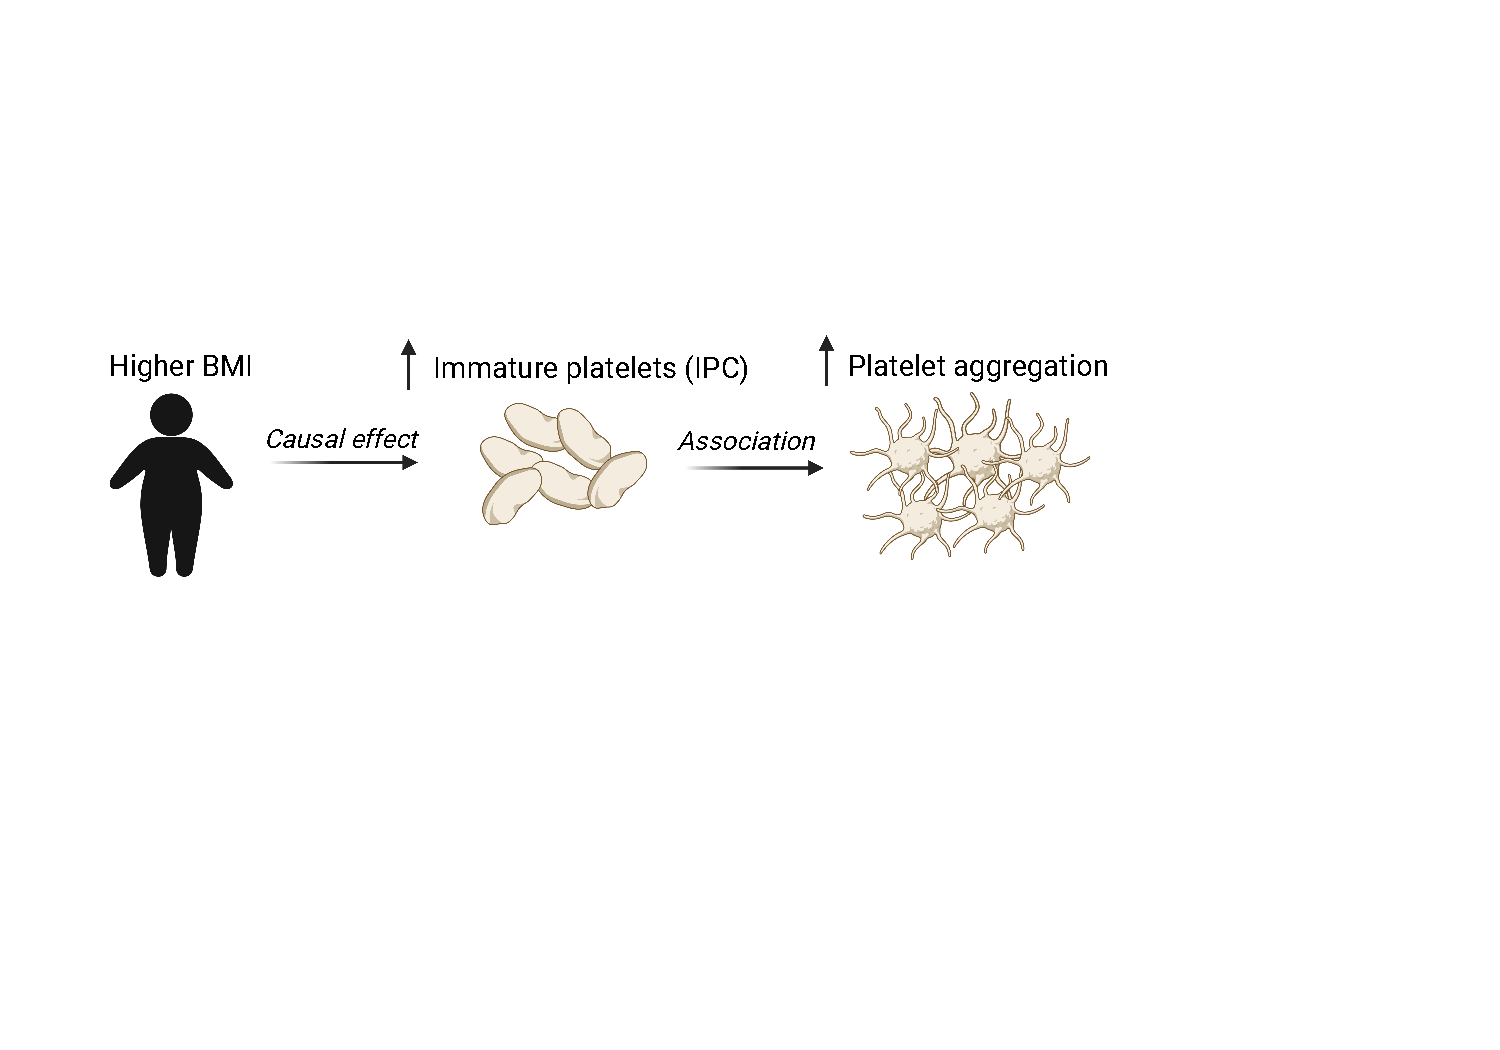
\includegraphics[width=0.85\linewidth,height=0.8\textheight]{figure/BMI_platelets/Visual_abstract} \caption{Graphical summary of findings}\label{fig:BMI-platelet-cartoon}
\end{figure}
\hypertarget{discussion}{%
\section{Discussion}\label{discussion}}

In this study we used data from 33,388 healthy blood donors to study the effect of BMI on platelet phenotypes including measures of count, size and maturity. The combination of observational and MR estimates suggested a positive causal effect of BMI on SFL and IPC. The observational analysis revealed a strong association between BMI and both PLT and PCT, however the MR estimates did not provide evidence to support this association as causal. Observational analysis using data from a cardiac surgery cohort provided evidence for a positive association between IPC and aggregation induced by adrenaline, TRAP6 and ADP.

The observational and MR analyses in the current study provide evidence for a positive association between BMI and both IPC and SFL. As IPC is derived using SFL, the measure of mRNA content, these measures are highly correlated. Whilst few studies have explored the direct association between BMI and immature platelet measures, there is some evidence for increased immature platelets in subjects with metabolic syndrome (MS) and subjects with type II diabetes compared with control subjects.\textsuperscript{46,47} In these studies, participants with MS or type II diabetes also had a higher BMI, which could be a possible cause of this increase in immature platelets. Indeed, evidence from our analysis suggests that BMI, independent of metabolic syndrome or type II diabetes, may causally influence IPC and SFL.

As IPC is an indirect measure of platelet production,\textsuperscript{39} these results suggest that an increased BMI may lead to an increased production of platelets. It has been reported that immature platelets have increased thrombotic potential\textsuperscript{39,56} and may be predictive of cardiovascular events,\textsuperscript{38,57} suggesting that an increase in the number of immature platelets may be of functional and clinical relevance. A follow-up analysis confirmed that higher IPC was associated with greater platelet aggregation independent of absolute platelet count within a cardiac surgery cohort. Positive associations were found between IPC and aggregation induced by adrenaline, TRAP-6 and ADP, suggesting general platelet hyperactivity with more immature platelets. A previous study in a coronary artery disease cohort also found a positive correlation between IPC and aggregation induced by arachidonic acid, collagen and ADP.\textsuperscript{56} These findings suggest that IPC can be used as a proxy for platelet hyperactivity within a cohort with a history of cardiovascular disease. Measures of immature platelets are currently not considered in the clinic when prescribing antiplatelet therapy, however if a higher immature platelet count is demonstrative of newly produced, hyperactive platelets then this could be important in guiding dosage regimes to ensure sufficient platelet inhibition.\textsuperscript{40} Observational studies have also found that patients with COVID-19 have elevated immature platelet counts and fraction, which could partly explain high rates COVID-19 induced thrombosis.\textsuperscript{59} Despite the association between BMI and IPC, there was less evidence for an effect of BMI on IPF. This lack of association may be because IPF is the proportion of immature platelets, therefore if someone had a higher number of immature platelets, but also a higher number of platelets overall (for example due to increased platelet lifespan), there would be no increase in the immature platelet fraction.

In general, previous studies have reported positive observational associations between BMI and both PLT and PCT.\textsuperscript{42} More direct measures of body fat such as total fat mass, waist-hip ratio and waist circumference have also been reported to be positively associated with both PLT and PCT;\textsuperscript{43} the observational evidence from the current study is in agreement with this. The MR analysis did not detect causal effects of BMI on measures of PLT/PCT, however the estimates were consistently positive. It is possible that IPC could be raised in absence of raised PLT as platelets may being produced at an increased rate, but could also be being destroyed at an increased rate. The small P values in the Wu-Hausman test for endogeneity for plateletcrit and platelet count variables support that the observational and MR estimates are different. Estimates could be biased due to confounding factors, reverse causation or other sources of bias. Possible routes of confounding could include stress, inflammation and nutrition, which could exert independent effects on both BMI and platelet count.

Both observational and MR estimates suggested that BMI is not associated with measures of platelet size, such as MPV and P-LCR. There are conflicting findings in the literature, with some studies suggesting that there is a positive association between BMI and MPV\textsuperscript{44} and others showing no association.\textsuperscript{42,43,45} The results of the current study suggest that associations seen previously between BMI and MPV are likely due to confounding of observational estimates. The lack of association between BMI and MPV may be surprising given a correlation coefficient of 0.62 between IPC and MPV. As BMI was positively associated with immature platelet count, and immature platelets tend to be larger, it may be surprising that BMI was not associated with measures of platelet size. However, immature platelets make up a small percentage of overall platelets (\textasciitilde3-6 \%),\textsuperscript{38,40} therefore the increase in immature platelets may not affect the overall median size of the whole platelet population.

Although this study suggests potential effects of BMI on platelet traits such as SFL and IPC, it does not provide mechanistic insight into how BMI exerts these effects. Previous studies have suggested that inflammation driven by adiposity can stimulate megakaryocyte proliferation, thereby increasing platelet numbers.\textsuperscript{43} There is evidence that inflammatory mediators such as interleukin-6 (IL-6) could be one such factor.\textsuperscript{60} Further study would be warranted to explore these mechanisms, as well as replicate the current findings, such as through independent population or clinical studies.

There are a few limitations to the study that should be recognised. Firstly, BMI was derived from self-reported height and weight. Although there is potential for this to bias observations, previous studies have found that self-reported BMI and BMI measured in the clinic are strongly associated.\textsuperscript{61} The GRS also associates with BMI to the extent expected. Secondly, there may be other confounders which were not recorded within INTERVAL and therefore could not be accounted for in our models, such as, socio-economic position, which may affect both BMI and risk of thrombosis. Therefore, residual confounding of observational estimates cannot be ruled out. With respect to the observational analysis conducted in COPTIC, the sample size is modest, which may limit power to detect associations. Furthermore, this cohort required cardiac surgery and therefore it is possible that associations found may not be generalizable to the wider population, as participants also displayed greater aggregatory responses than the reference ranges.\textsuperscript{62} However, these findings do indicate that immature platelets may be a biomarker of platelet hyperactivity in patients with a history of cardiovascular disease. It is important to note that the anticoagulant used (EDTA) has been reported to affect platelet parameters, such as increasing MPV and decreasing PLT.\textsuperscript{63} Despite this, EDTA is the standard anticoagulant used for full blood counts in the NHS. The Sysmex analyzers used in INTERVAL and COPTIC were different models, however, it has been shown that there is strong association between platelet measures between the XE and newer XN analyzers.\textsuperscript{64}

Altogether, we show observational and MR evidence that an increased BMI is associated with an increase in number of immature platelets. Observational evidence indicates that higher immature platelet count is associated with enhanced aggregation in a cardiac surgery cohort. Together, these results indicate that higher BMI may enhance platelet function and thrombosis by increasing platelet production and immature platelet count.

\hypertarget{the-effect-of-obesity-on-platelet-function-a-clinical-pilot-study}{%
\chapter{The effect of obesity on platelet function: a clinical pilot study}\label{the-effect-of-obesity-on-platelet-function-a-clinical-pilot-study}}

The following results section is a clinical study. Recruitment into this study has been severely affected by COVID-19 as we had approvals to start recruitment in March 2020. All data in this chapter was collected by myself, apart from the platelet-neutrophil assay data, which was performed by Dr Chris Williams due to time constraints when receiving patient samples. The proteomic data was analysed by the Proteomics facility at the University of Bristol.

\hypertarget{background-3}{%
\section{Background}\label{background-3}}

\hypertarget{obesity-is-associated-with-cardiovascular-events-e.g.-heart-attacks-and-stroke}{%
\subsection{Obesity is associated with cardiovascular events e.g.~heart attacks and stroke}\label{obesity-is-associated-with-cardiovascular-events-e.g.-heart-attacks-and-stroke}}

\hypertarget{platelets-are-a-key-cell-involved-in-thrombosis}{%
\subsection{Platelets are a key cell involved in thrombosis}\label{platelets-are-a-key-cell-involved-in-thrombosis}}

The aims of this clinical study were to determine whether an increased BMI is associated with an increase in platelet function and an alteration in platelet signalling compared to healthy controls. In light of the recent pandemic

\hypertarget{methods-1}{%
\section{Methods}\label{methods-1}}

\hypertarget{materials}{%
\subsection{Materials}\label{materials}}

Protease-activated receptor 1 (PAR-1)-activating peptide (SFLLRN-NH2) was from Bachem (Bubendorf, Switzerland), crosslinked collagen-related peptide (CRP-XL) from Prof.~Richard Farndale (Department of Biochemistry, University of Cambridge, UK). Adenosine diphosphate (ADP) was from Sigma-Aldrich (Poole, UK). cOmplete mini protease inhibitor tablets and phosSTOP phosphatase inhibitors were from Roche Life Sciences (Welwyn Garden City, UK). The Pierce bicinchoninic acid (BCA) assay was from ThermoFisher Scientific (Altrincham, UK). Sodium Citrate Vacutainer® tubes, FixLyse, PE-Cy5-conjugated anti-CD42b, FITC-conjugated CD61 antibody, Fc block, PE-conjugated human platelet GPVI antibody, PAC1-FITC and anti-CD62P-PE antibodies were from BD (Wokingham, UK). FITC-conjugated anti-human CD41 and CD42b antibody were from BioLegend (London, UK).

\hypertarget{study-population-1}{%
\subsection{Study population}\label{study-population-1}}

This study was approved by the London Riverside Research Ethics Committee. Bariatric patients with a body mass index of \textgreater40kg/m\textsuperscript{2} were recruited from the Department of Bariatric and Metabolic Surgery at Southmead Hospital, Bristol. Participants with a BMI between 18 and 25 kg/m\textsuperscript{2} were recruited from the University of Bristol. Inclusion criteria for participants were: aged 18 years and over and able to give written informed consent. Participants were excluded if they were pregnant or lactating, had any known clotting or bleeding disorders (e.g.~von Willebrand disease or drug-induced thrombocytopenia), or if they had taken any antiplatelet medication within the previous 14 days such as clopidogrel, ticagrelor or aspirin. Recruitment occurred between May and June 2021. As a pilot study, a total of four bariatric patients with obesity and four control participants were recruited. Bariatric patients donated blood before bariatric surgery.

\hypertarget{isolation-of-platelet-rich-plasma-prp-and-platelet-lysates}{%
\subsection{Isolation of platelet rich plasma (PRP) and platelet lysates}\label{isolation-of-platelet-rich-plasma-prp-and-platelet-lysates}}

Blood was taken by venipuncture into vacutainers containing sodium citrate (3.2\%). Blood was centrifuged (1000 RPM, 17 mins). PRP was isolated and diluted 1:40 in HEPES Tyrode's (145 mM NaCl, 3 mM KCl, 0.5 mM Na\textsubscript{2}HPO\textsubscript{4}, 1 mM MgS0\textsubscript{4}.7H\textsubscript{2}O, 10 mM HEPES, pH 7.4, 0.1\% {[}w/v{]} D‐glucose). To create platelet lysates, acid citrate dextrose (1:7) and apyrase (0.02 U/mL) were added to isolated PRP. PRP was centrifuged (1700 RPM, 10 mins). Platelets were double washed in CGS buffer (120 mM NaCl, 25.8 mM sodium citrate dihydrate, 0.1\% {[}w/v{]} D‐glucose, 0.02 U/mL apyrase, pH 6.5). Platelets were resuspended in radioimmunoprecipitation assay buffer (RIPA: 25 mM HEPES, 200 mM NaCL, 1mM EDTA, 1 \% (v/v) NP40, 0.5 \% (w/v) sodium deoxychelate, 0.1 \% (w/v) SDS) supplemented with a protease and phosphatase inhibitor for 10 minutes on ice. Lysates were centrifuged at 10000 RPM, at 4°C for 5 minutes. Supernatant was removed and a bicinchoninic acid (BCA) assay was performed to calculate sample protein concentrations. Samples were stored in a -80°C freezer until used for proteomics analysis.

\hypertarget{platelet-parameters-measured-by-sysmex}{%
\subsection{Platelet parameters measured by Sysmex}\label{platelet-parameters-measured-by-sysmex}}

Citrated whole blood (200 uL) was analysed using the Sysmex XE-2100 haematology analyser. Platelet readouts were platelet count (PLT), immature platelet fraction (IPF), immature platelet count (IPC), side fluorescence (SFL, a measure of mRNA content), forward scatter (FSC, a measure of platelet size), side scatter (SSC, a measure of granularity).

\hypertarget{integrin-ux3b1iibux3b23-activation-and-p-selectin-expression-measured-by-flow-cytometry}{%
\subsection{\texorpdfstring{Integrin α\textsubscript{IIb}β\textsubscript{3} activation and P-selectin expression measured by flow cytometry}{Integrin αIIbβ3 activation and P-selectin expression measured by flow cytometry}}\label{integrin-ux3b1iibux3b23-activation-and-p-selectin-expression-measured-by-flow-cytometry}}

Isolated PRP was diluted 1:40 in HEPES Tyrode's, with the antibodies FITC-conjugated PAC1 and PE-conjugated CD62P in a 2:1 ratio. Master mix was added to pre-prepared vacuum packed 96 well plates to a final folume of 50 uL. Agonists used were PAR1-AP, ADP and CRP, which were freeze-dried onto the plates,\textsuperscript{65} as well as HEPES Tyrode's which was used for a measurement of unstimulated integrin α\textsubscript{IIb}β\textsubscript{3} activation and P-selectin expression. Platelets were stimulated with agonists for 10 minutes and were fixed with 2 \% paraformaldehyde (PFA) for 20 minutes. Plates were analysed using the BD Accuri C6 Plus flow cytometer (BD Biosciences, Wokingham, UK), where the median fluorescence intensity was derived from 10,000 gated platelets.

\hypertarget{surface-receptor-levels-measured-by-flow-cytometry}{%
\subsection{Surface receptor levels measured by flow cytometry}\label{surface-receptor-levels-measured-by-flow-cytometry}}

Diluted PRP (1:40) was used for unstimulated surface receptor detection. Antibody was added (1:10 v/v) to a final volume of 50 uL. Antibodies used include anti-human CD41, CD42b, CD61 (FITC-conjugated) and GPVI and CD110 (PE-conjugated). Platelets were gated and the median fluorescence was reported from a total of 10,000 events.

\hypertarget{platelet-neutrophil-assay-measured-by-flow-cytometry}{%
\subsection{Platelet-neutrophil assay measured by flow cytometry}\label{platelet-neutrophil-assay-measured-by-flow-cytometry}}

Citrated whole blood was diluted 1 in 10 in HEPES-Tyrode's buffer and incubated with FITC-conjugated anti-CD41 and PE-conjugated anti-C45 antibodies at room temperature for 15 mins. Samples were either stimulated (+ 5 ug/mL CRP) or unstimulated (+ vehicle). Samples were fixed with FixLyse for 10 minutes, followed by 4 \% PFA for 10 minutes. Fluorescence was quantified using the flow cytometer, where 1000 neutrophil events were analysed based on a gating of CD45 and SSC parameters. Aggregates of platelets and neutrophils were defined by being both CD41+ and CD45+.

\hypertarget{tandem-mass-tag-mass-spectrometry-tmt-ms-quantification-of-platelet-proteins}{%
\subsection{Tandem Mass Tag Mass Spectrometry (TMT-MS) quantification of platelet proteins}\label{tandem-mass-tag-mass-spectrometry-tmt-ms-quantification-of-platelet-proteins}}

Platelet lysate samples (50 ug total protein) were digested with trypsin and labelled with TMT 15 plex reagents (Thermo Fisher Scientific, Loughborough, UK). Labelled samples were pooled. The pooled sample was evaporated to dryness then resuspended in formic acid (5\%). The pooled sample was then desalted using a SepPak cartridge (Waters, Milford, Massachussetts, USA). Eluate from the SepPak cartridge was evaporated to dryness and resuspended prior to fractionation by high pH reversed-phase chromatography using an Ultimate 3000 liquid chromatography system (Thermo Fisher Scientific). Further fractionation occurred using high pH RP fractions using the Ulitamte 3000 nano-LC system in line with an Orbitrap Fusion Tribrid Mass Spectrometer (Thermo Fisher Scientific).

\hypertarget{statistical-analysis-1}{%
\subsection{Statistical analysis}\label{statistical-analysis-1}}

Data was analysed using GraphPad Prism 8. If data displayed a normal distribution (based on Shapiro-Wilk p-value and W statistic), a parametric test was used (e.g.~unpaired t-test or one way ANOVA), otherwise a nonparametric test was used. Concentration-response curve were plotted using a four parameter variable slope. To compare concentration-response curve parameters, logEC50s and curve maxes were compared. A Fisher's exact test was used to compare proportions of categorical variables. Due to limited power, caution should be taken when considering p-values.

\hypertarget{results-1}{%
\section{Results}\label{results-1}}

\hypertarget{participant-characteristics}{%
\subsection{Participant characteristics}\label{participant-characteristics}}

The characteristics of participants included in the study are shown in Table \ref{tab:obesity-platelets-participants}. The mean BMI in the control group was 21.8 kg/m\textsuperscript{2} (SD 2.1 kg/m\textsuperscript{2}) and 49.3 kg/m\textsuperscript{2} (SD 8.8 kg/m\textsuperscript{2}). Participants in the control group and bariatric patient group were age and sex matched. Bariatric patients exhibited similar smoking habits to control participants, however they displayed increased rates of T2D and previous symptomatic COVID-19 infection.
\begin{table}

\caption{\label{tab:obesity-platelets-participants}Characteristics of included participants}
\centering
\begin{tabu} to \linewidth {>{\raggedright\arraybackslash}p{3cm}>{\raggedright}X>{\raggedright}X>{\raggedright}X}
\toprule
Variable & Control mean (SD) or \% & Bariatric patient mean (SD) or \% & P value for difference\\
\midrule
Age & 42.2 (14.1) & 46 (18.0) & 0.77\\
Sex & 75 \% & 75 \% & 1\\
Body mass index (kg/m2) & 21.8 (2.1) & 49.3 (8.8) & 9e-04\\
Smoker & 0 \% & 0 \% & 1\\
Hypertensive (140/90 mmHg) & 0 \% & 25 \% & 1\\
\addlinespace
Type 2 Diabetes & 0 \% & 50 \% & 0.43\\
Type 2 Diabetes medication & NA &  & NA\\
\hspace{1em}Metformin &  & 25 \% & \\
\hspace{1em}Dapagliflozin &  & 25 \% & \\
\hspace{1em}Dulaglutide &  & 25 \% & \\
\addlinespace
Previous COVID-19 infection & 0 \% & 75 \% & 0.14\\
\bottomrule
\end{tabu}
\end{table}
\hypertarget{platelet-parameters}{%
\subsection{Platelet parameters}\label{platelet-parameters}}

Platelet traits measured by Sysmex were compared across bariatric and control groups (Table \ref(tab:obesity-platelets-parameters)). There was no statistical evidence for an effect of obesity on platelet parameters. However, IPC and IPF did display larger mean values compared to controls, but they also had relatively large SDs in the bariatric patient group. A higher N would be required to detect whether there is any difference between groups.
\begin{table}

\caption{\label{tab:obesity-platelets-parameters}Platelet traits measured by Sysmex XE-2100}
\centering
\begin{tabu} to \linewidth {>{\raggedright}X>{\raggedright}X>{\raggedright}X>{\raggedleft}X}
\toprule
Variable & Control mean (SD) & Bariatric patient mean (SD) & P value for difference\\
\midrule
Platelet count & 257.8 (29.1) & 235.8 (61.5) & 0.54\\
Immature platelet fraction & 3.8 (2.3) & 7.3 (8.3) & 0.44\\
Immature platelet count & 9.3 (4.9) & 16.3 (16.3) & 0.45\\
Side fluorescence & 82.0 (5.8) & 85.1 (9.8) & 0.61\\
Forward scatter & 53.8 (5.5) & 60.5 (8.8) & 0.24\\
\addlinespace
Side scatter & 40.3 (1.1) & 41.8 (3.0) & 0.37\\
\bottomrule
\end{tabu}
\end{table}
\hypertarget{basal-receptors}{%
\subsection{Basal receptors}\label{basal-receptors}}

Unstimulated platelet receptor levels were compared across bariatric patient and control participant groups. Basal integrin α\textsubscript{IIb}β\textsubscript{3} activation and P-selectin expression were similar across groups. Similarly, other platelet receptors were not different across groups.



\begin{figure}
\includegraphics{figure/Bariatric_study/Basal_surface_receptors} \caption[(ref:scaption)]{(ref:caption)}\label{fig:basal-integrin-pselectin-receptor-bariatric}
\end{figure}
\hypertarget{agonist-induced-integrin-ux3b1iibux3b23-and-p-selectin-expression}{%
\subsection{\texorpdfstring{Agonist-induced integrin α\textsubscript{IIb}β\textsubscript{3} and P-selectin expression}{Agonist-induced integrin αIIbβ3 and P-selectin expression}}\label{agonist-induced-integrin-ux3b1iibux3b23-and-p-selectin-expression}}

Markers of platelet activation were compared in response to different platelet agonists.



\begin{figure}
\includegraphics{figure/Bariatric_study/Agonist_Integrin_Pselectin} \caption[Concentration response curves of integrin activation and P-selectin expression]{Concentration response curves in diluted PRP of: integrin activation in response to A) PAR1-AP, B) ADP and C) CRP and P-selectin expression in response to D) PAR1-AP, E) ADP, F) CRP. N=4.}\label{fig:agonist-integrin-pselectin}
\end{figure}
\hypertarget{platelet-neutrophil-aggregates}{%
\subsection{Platelet-neutrophil aggregates}\label{platelet-neutrophil-aggregates}}



\begin{figure}
\includegraphics{figure/Bariatric_study/Plt-neu_aggregates} \caption[Comparison of platelet-neutrophil aggregates]{Comparison of platelet-neutrohpil aggregates across bariatric patient and control participant groups in unstimulated and stimulated (5 ug/mL CRP) conditions. N=4. P-values provided for the results of a two-way ANOVA with Sidak's multiple comparisons tests.}\label{fig:platelet-neutrophil}
\end{figure}
\hypertarget{proteomics}{%
\subsection{Proteomics}\label{proteomics}}

\hypertarget{pca}{%
\subsubsection{PCA}\label{pca}}

\hypertarget{volcano-plot}{%
\subsection{Volcano plot}\label{volcano-plot}}

\hypertarget{discussion-1}{%
\section{Discussion}\label{discussion-1}}

This study has explored the effect of obesity on platelet parameters and platelet function. Initial analyses are inconclusive as the experiment lacks power. Despite this, optimisation of experimental techniques used within the study provides a means of exploring effects in the future.

Overall effects
We have been able to optimise common platelet experiments to be more high throughput for patient studies.
Limitations - what we initially aimed to do wasnt possible so power is limited.

\hypertarget{pathways-linking-bmi-and-platelet-function-do-the-chemokines-mdc-and-tarc-play-a-role}{%
\chapter{Pathways linking BMI and platelet function: do the chemokines MDC and TARC play a role?}\label{pathways-linking-bmi-and-platelet-function-do-the-chemokines-mdc-and-tarc-play-a-role}}

\hypertarget{background-4}{%
\section{Background}\label{background-4}}

Why these? Suggested they could be raised in obesity.

\hypertarget{methods-2}{%
\section{Methods}\label{methods-2}}

\hypertarget{materials-1}{%
\subsection{Materials}\label{materials-1}}

\hypertarget{isolation-of-human-platelets}{%
\subsection{Isolation of human platelets}\label{isolation-of-human-platelets}}

Fresh human venous blood was obtained from healthy volunteers by venipuncture. Blood was taken into the syringe with a 1 in 10 volume of 4 \% trisodium citrate, then mixed with a 1 in 7 volume of acid citrate dextrose (ACD). Blood was placed into 5 mL LP4 tubes then centrifuged at 1000 revolutions per minute (RPM) for 17 minutes. Platelet rich plasma (PRP) was extracted. PRP was supplemented with inhibitors such as 0.02 U/mL apyrase, 140 nM PGE1 or 10 µM indomethacin (exact inhibitors for each experiment used will be shown in results). Supplemented PRP was either used for the experiment of centrifuged for a further 10 minutes at 1700 RPM. Platelet poor plasma (PPP) was removed leaving a platelet pellet. This pellet was resuspended in HEPES Tyrode's (supplemented with 0.1 \% glucose and 0.02 U/mL apyrase, and 10 µM indomethacin if already applied to PRP). Platelets were counted using a Z1 coulter particle counter by diluting 1 in 2000 in 10 mL MQ water. Platelets were diluted further using the supplemented HEPES Tyrode's to a platelet concentration of 4 x 10\textsuperscript{8}/mL and left to rest for 30 mins in a 30°C water bath.

\hypertarget{platelet-aggregation}{%
\subsection{Platelet aggregation}\label{platelet-aggregation}}

\hypertarget{flow-cytometry-integrin-ux3b1iibux3b23-activation-and-p-selectin-expression}{%
\subsection{\texorpdfstring{Flow cytometry: integrin α\textsubscript{IIb}β\textsubscript{3} activation and P-selectin expression}{Flow cytometry: integrin αIIbβ3 activation and P-selectin expression}}\label{flow-cytometry-integrin-ux3b1iibux3b23-activation-and-p-selectin-expression}}

Platelets were diluted to a concentration of 2 x 10\textsuperscript{7}/mL using supplemented HEPES Tyrode's buffer. Platelets were incubated with 200 ng/ml MDC, TARC or vehicle for 5 mins, then added to wells in a 96 well plate already containing a mixture of PAC1 and CD62P antibodies (in a 2:1 ratio), as well as increasing concentrations of PAR1-AP. After a further 5 minutes, platelets were fixed with 1 \% paraformaldehyde (PFA). Plates were read using a BD Accuri C6 Plus flow cytometer. The relative fluorescence of the antibody in each well was measured over 10,000 platelets and median statistics were used.

\hypertarget{flow-cytometry-phospho-vasp}{%
\subsection{Flow cytometry: phospho-VASP}\label{flow-cytometry-phospho-vasp}}

\hypertarget{western-blotting}{%
\subsection{Western blotting}\label{western-blotting}}

\hypertarget{calcium-mobilisation}{%
\subsection{Calcium mobilisation}\label{calcium-mobilisation}}

\hypertarget{plate-platelet-aggregation}{%
\subsection{Plate platelet aggregation}\label{plate-platelet-aggregation}}

\hypertarget{results-2}{%
\section{Results}\label{results-2}}

\hypertarget{priming-effects-of-mdc-and-tarc-on-platelet-aggregation-in-washed-platelets-using-light-transmittance-aggregometry}{%
\subsection{Priming effects of MDC and TARC on platelet aggregation in washed platelets using light transmittance aggregometry}\label{priming-effects-of-mdc-and-tarc-on-platelet-aggregation-in-washed-platelets-using-light-transmittance-aggregometry}}



\begin{figure}
\includegraphics{figure/Chemokines/Layouts/MDC_TARC_aggregation_PAR1} \caption[The priming effect of the chemokines MDC and TARC on PAR1-AP induced platelet aggregation in washed platelets]{Washed platelets at 2x10\textsuperscript{8}/mL were preincubated with MDC or TARC (5 mins) before application of PAR1-AP-induced aggregation (5 mins). A) Raw aggregation trace comparing the effect of vehicle, 200 ng/mL MDC or 200 ng/mL TARC on PAR1-AP induced aggregation. B) Bar chart comparing the maximum aggregation reached when adding vehicle, MDC or TARC. C) Bar chart comparing the area under the curve of the aggregation trace in response to vehicle, MDC or TARC. Results analysed with a repeated measures one-way ANOVA with Dunnett's multiple comparisons. N=7. Mean+SEM displayed.}\label{fig:MDC-TARC-agg}
\end{figure}
\hypertarget{priming-effects-of-mdc-and-tarc-on-par1-ap-induced-integrin-ux3b1iibux3b23-activation-and-p-selectin-expression}{%
\subsection{\texorpdfstring{Priming effects of MDC and TARC on PAR1-AP induced integrin α\textsubscript{IIb}β\textsubscript{3} activation and P-selectin expression}{Priming effects of MDC and TARC on PAR1-AP induced integrin αIIbβ3 activation and P-selectin expression}}\label{priming-effects-of-mdc-and-tarc-on-par1-ap-induced-integrin-ux3b1iibux3b23-activation-and-p-selectin-expression}}



\begin{figure}
\includegraphics{figure/Chemokines/Layouts/P-selectin_integrin_MDC_TARC} \caption[The priming effect of the chemokines MDC and TARC on PAR1-AP induced α\textsubscript{IIb}β\textsubscript{3} activation and P-selectin expression]{Washed platelets at 2x10\textsuperscript{7}/mL were preincubated with MDC or TARC (5 mins) before application of PAR1-AP (5 mins). Integrin α\textsubscript{IIb}β\textsubscript{3} activation and P-selectin expression were measured using flow cytometry. A) The effect of vehicle, 200 ng/mL MDC or 200 ng/mL TARC on PAR1-AP induced α\textsubscript{IIb}β\textsubscript{3} activation. B) The effect of vehicle, MDC or TARC on PAR1-AP induced P-selectin expression. LogEC50s compared using a one-way ANOVA with Dunnett's multiple comparisons in Table \ref{tab:chemokines-integrin-pselectin}}\label{fig:MDC-TARC-integrin-pselectin}
\end{figure}
\begin{landscape}\begin{table}

\caption{\label{tab:chemokines-integrin-pselectin}Comparison of the effect of MDC and TARC on the logEC50 for PAR1-AP induced integrin activation and P-selectin expression compared with a one-way ANOVA (N=4)}
\centering
\begin{tabu} to \linewidth {>{\raggedright}X>{\raggedright}X>{\raggedright}X>{\raggedright}X>{\raggedright}X>{\raggedright}X>{\raggedright}X}
\toprule
Condition & Integrin activation logEC50 (M) & Integrin SEM & Integrin P value & P-selectin logEC50 (M) & P-selectin SEM & P-selectin p value\\
\midrule
Vehicle & -5.54 & 0.1 &  & -5.36 & 0.07 & \\
MDC & -5.66 & 0.08 & 0.019 & -5.44 & 0.07 & 0.006\\
TARC & -5.64 & 0.11 & 0.014 & -5.46 & 0.11 & 0.21\\
\bottomrule
\end{tabu}
\end{table}
\end{landscape}
\hypertarget{effects-of-mdc-and-tarc-on-par1-ap-induced-ps-exposure}{%
\section{Effects of MDC and TARC on PAR1-AP induced PS exposure}\label{effects-of-mdc-and-tarc-on-par1-ap-induced-ps-exposure}}



\begin{figure}
\includegraphics{figure/Chemokines/Layouts/MDC_TARC_PS_exposure_layout} \caption[The effect of the chemokines MDC and TARC on PAR1-AP induced PS exposure]{A) Washed platelets at 2x10\textsuperscript{7}/mL were preincubated with vehicle, 200ng/mL MDC or 200 ng/mL TARC (5 mins) before application of increasing concentrations of PAR1-AP (10 mins). PS exposure was measured using flow cytometry (N=4). B) Bar chart comparing the effect of vehicle, MDC or TARC on the logEC50s of PAR1-AP induced PS exposure. LogEC50s compared by a Friedman's test.}\label{fig:MDC-TARC-PS-exposure}
\end{figure}
\hypertarget{mechanism-of-mdc-and-tarc-priming-in-washed-platelets}{%
\subsection{Mechanism of MDC and TARC priming in washed platelets}\label{mechanism-of-mdc-and-tarc-priming-in-washed-platelets}}

\hypertarget{effects-of-mdc-and-tarc-on-phospho-vasp-levels}{%
\subsection{Effects of MDC and TARC on phospho-VASP levels}\label{effects-of-mdc-and-tarc-on-phospho-vasp-levels}}



\begin{figure}
\includegraphics{figure/Chemokines/Layouts/MDC_TARC_VASP_FACS_logec50} \caption[The effect of the chemokines MDC and TARC on phospho-VASP levels]{A) Washed platelets at 1x10\textsuperscript{8}/mL were preincubated with vehicle, 200ng/mL MDC, 200 ng/mL TARC or 10 uM ADP (5 mins) before application of increasing concentrations of PGE\textsubscript{1} (5 mins). PS exposure was measured using flow cytometry (N=3). B) Bar chart of the logEC50s of each concentration response curve from A. LogEC50s were compared using a one-way ANOVA with Dunnett's multiple comparisons.}\label{fig:MDC-TARC-VASP-FACS}
\end{figure}


\begin{figure}
\includegraphics{figure/Chemokines/MDC_TARC_VASP_blot} \caption[A representative blot of the effect of MDC, TARC and ADP on PGE\textsubscript{1} stimulated phospho-VASP.]{A representative blot of the effect of 200 ng/mL MDC, 200 ng/mL TARC and 10 uM ADP on phospho-VASP at Serine 157 and 239 in the presence of increasing concentrations of PGE\textsubscript{1}}\label{fig:MDC-TARC-wp-WB-VASP}
\end{figure}


\begin{figure}
\includegraphics{figure/Chemokines/Layouts/MDC_TARC_WB_VASP} \caption[Quantification of the effect of MDC, TARC and ADP on PGE\textsubscript{1} stimulated phospho-VASP.]{Bar charts of the effect of 200 ng/mL MDC, 200 ng/mL TARC and 10 uM ADP on phospho-VASP at A) Serine 239 in the absence of PGE\textsubscript{1}, B) Serine 239 in the presence of 100 nM PGE\textsubscript{1}, C) Serine 157 in the absence of PGE\textsubscript{1}, D) Serine 157 in the presence of 100 nM PGE\textsubscript{1}. N=4. Results analysed with a repeated measures one-way ANOVA with Dunnett's Multiple comparisons.}\label{fig:MDC-TARC-wp-VASP-bar}
\end{figure}
\hypertarget{effects-of-mdc-and-tarc-alone-on-aggregation-in-washed-platelets}{%
\subsection{Effects of MDC and TARC alone on aggregation in washed platelets}\label{effects-of-mdc-and-tarc-alone-on-aggregation-in-washed-platelets}}



\begin{figure}
\includegraphics{figure/Chemokines/Layouts/MDC_TARC_alone_wp_aggregation} \caption[The effect of the chemokines MDC and TARC alone on aggregation in washed platelets]{A-C) Washed platelets at 2x10\textsuperscript{8}/mL were stimulated with vehicle, 200ng/mL MDC, 200 ng/mL TARC or 1 uM PAR1-AP (5 mins). Aggregation was measured using light transmittance aggregometry. Each graph is a representative trace from a separate donor}\label{fig:MDC-TARC-wp-alone-aggregation}
\end{figure}
\hypertarget{effects-of-mdc-and-tarc-alone-on-calcium-mobilisation}{%
\subsection{Effects of MDC and TARC alone on calcium mobilisation}\label{effects-of-mdc-and-tarc-alone-on-calcium-mobilisation}}



\begin{figure}
\includegraphics{figure/Chemokines/Layouts/MDC_TARC_calcium_wp} \caption[The effect of ADP and the chemokines MDC and TARC alone on calcium mobilisation in washed platelets.]{Washed platelets at 2x10\textsuperscript{8}/mL loaded with Fura-2 were stimulated with increasing concentrations of A) ADP or B) 200ng/mL MDC or 200 ng/mL TARC. Area under curve represents the free calcium and is ratio of fluorescence at wavelengths 340:380 nm.}\label{fig:MDC-TARC-wp-calcium}
\end{figure}
\hypertarget{priming-effects-of-mdc-and-tarc-on-platelet-aggregation-in-prp}{%
\subsection{Priming effects of MDC and TARC on platelet aggregation in PRP}\label{priming-effects-of-mdc-and-tarc-on-platelet-aggregation-in-prp}}



\begin{figure}
\includegraphics{figure/Chemokines/Layouts/MDC_TARC_PRP_plate_agg} \caption[The priming effect of the chemokines MDC and TARC on PAR1-AP induced platelet aggregation in PRP using plate aggregation]{PRP was preincubated with MDC or TARC (5 mins) before application of PAR1-AP-and aggregation induced by a plate shaker (5 mins). A) A concentration response curve of the effect of vehicle, 200 ng/mL MDC or 200 ng/mL TARC on PAR1-AP induced aggregation. N=7. B) A bar chart of the logEC50s of the PAR1-AP concentration response curve in the presence of vehicle, MDC or TARC. Results analysed using a repeated measures one-way ANOVA with Dunnett's multiple comparisons. N=7.}\label{fig:MDC-TARC-agg-PRP}
\end{figure}
\hypertarget{mechanisms-of-the-effect-of-mdc-on-platelet-aggregation-in-prp}{%
\subsection{Mechanisms of the effect of MDC on platelet aggregation in PRP}\label{mechanisms-of-the-effect-of-mdc-on-platelet-aggregation-in-prp}}



\begin{figure}
\includegraphics{figure/Chemokines/Layouts/MDC_inhibitors_aggregation_traces} \caption[Example aggregation traces of the effect of inhibitors on MDC induced platelet aggregation in PRP.
(ref:caption11)]{(ref:caption11)}\label{fig:MDC-PRP-agg-trace}
\end{figure}


\begin{figure}
\includegraphics{figure/Chemokines/Layouts/PAR1_MDC_inhibitors_aggregation} \caption[The effect of inhibitors on PAR1-AP and MDC induced aggregation in PRP.]{Results analysed with a repeated measures one-way ANOVA with Dunnett's Multiple comparisons.}\label{fig:MDC-PRP-agg-bar}
\end{figure}
\hypertarget{discussion-2}{%
\section{Discussion}\label{discussion-2}}

\hypertarget{BMI-protein-MR}{%
\chapter{Effects of adiposity on the human plasma proteome: Observational and Mendelian randomization estimates}\label{BMI-protein-MR}}

The work within this chapter has been published in the International Journal of Obesity.\textsuperscript{33} I am the first author of the publication; I performed all analyses, created all figures and tables and wrote the manuscript.

Supplementary Tables 1-7 can be found here \url{https://github.com/lucygoudswaard/mythesis/blob/master/index/figure/BMI_protein_INTERVAL/BMI_protein_supplementary_Tables.xlsx}

\hypertarget{introduction-1}{%
\section{Introduction}\label{introduction-1}}

Obesity has tripled worldwide since 1975, now affecting around 40\% of adults in the United States and 26\% of adults in the UK.\textsuperscript{1} The average body mass index (BMI) of the UK adult population is now in the conventional `overweight' category (BMI between 25 and 30 kg/m\textsuperscript{2})\textsuperscript{3} and `overweight' is now more common than `normal-weight' in middle age in many high-income countries.\textsuperscript{4} BMI is often used as a proxy for adiposity given high correlations between BMI and more objectively measured fat mass indices.\textsuperscript{20} Higher adiposity is a major risk factor for various noncommunicable diseases including type II diabetes, cardiovascular diseases, musculoskeletal diseases, and cancer,\textsuperscript{7--9} which collectively put a strain on health services.\textsuperscript{11} These BMI-disease associations are supported by prospective observational studies and, more recently, by Mendelian randomization (MR) studies,\textsuperscript{13--15} which use genetic variation reliably associated with BMI to re-estimate effects of BMI on disease outcomes. Given the properties of genetic variation, this method helps to overcome issues such as confounding and reverse causation which commonly occur with observational studies.\textsuperscript{66}
Despite MR studies supporting a causal role of adiposity for cardiometabolic diseases, and randomised trials supporting the effectiveness of weight loss in reducing disease risk,\textsuperscript{16} the molecular footprint of adiposity is not well understood. Previous studies have largely focused on the impact of higher BMI on the lipidome including traits such as cholesterol and triglycerides in lipoprotein subtypes (e.g.~low-density lipoprotein (LDL) and high-density lipoprotein (HDL) particles)\textsuperscript{20,21} and on inflammatory molecules such as C-reactive protein (CRP).\textsuperscript{21,23}
A benefit of studying the systematic effects of BMI on the circulating proteome is that proteins are often more suitable pharmacological targets than metabolites. Efforts to study the effect of BMI on the proteome have generally been in an observational framework.\textsuperscript{24} It is estimated that 25\% of proteins in the human proteome circulate in blood,\textsuperscript{25} which is important as the majority of druggable targets are such proteins.\textsuperscript{22} Studying the effect of BMI on a large set of proteins has only recently become possible with newly developed proteomic technologies such as the SomaLogic platform, with the ability to quantify enzymes, protein kinases and transport proteins with unprecedented sensitivity.\textsuperscript{67} Utilisation of SomaLogic within a trial or cohort setting has recently become more widespread, such as within the INTERVAL study, a UK cohort of blood donors.\textsuperscript{68} There is evidence that proteins which change as a result of a higher BMI may contribute to cardiometabolic disease: identification of such proteins is important in understanding how higher BMI causes disease and to identify targets which may benefit from pharmacological intervention.
In this study, we aimed to measure associations between adiposity and the human proteome and to also estimate the underlying effects in a causal framework. Using data on 2737 participants from INTERVAL, we estimated effects of BMI on 4034 (3622 unique) plasma protein traits, in both observational and MR frameworks. We examined the agreement between effect estimates from different methods and performed enrichment analyses of the most strongly altered proteins to map their potential relevance to disease.

\hypertarget{methods-3}{%
\section{Methods}\label{methods-3}}

\hypertarget{study-population-2}{%
\subsection{Study population}\label{study-population-2}}

INTERVAL is a prospective cohort study which was initially a randomised trial that aimed to test the efficiency and safety of reducing the time between whole blood donation in approximately 50000 participants.\textsuperscript{48} Upon informed consent, eligible participants who were: aged 18 years and over, willing to complete online questionnaires and without a self-reported history of major disease were recruited between June 11th, 2012 and June 15th, 2014 from 25 National Health Service Blood and Transplant (NHSBT) centres across England. Participants filled out questionnaires including self-reported height and weight, smoking frequency and alcohol consumption. Blood samples were taken at baseline which were analysed for full blood counts and blood biomarkers. This study was approved by Cambridge (East) Research Ethics Committee. Access to the data was granted by the Data Access Committee.
The present study was conducted on a random subset of participants from INTERVAL who had basic phenotype data and plasma proteins measured by SomaLogic. This included up to 2737 participants mostly of European descent across analyses described below.

\hypertarget{assessment-of-bmi-and-covariables}{%
\subsection{Assessment of BMI and covariables}\label{assessment-of-bmi-and-covariables}}

Participants completed online questionnaires wherein they reported their height and weight. BMI was calculated as weight in kilograms divided by the square of their height in metres (kg/m\textsuperscript{2}). Available covariables were age, sex, previous or current smoking frequency (in three categories of: never, occasional, most days or every day) and alcohol intake frequency (in four categories of: rarely, less than once a week, 1-2 times a week, 3-5 times a week or most days). These covariables were chosen as they were measured in the INTERVAL collection and are measures which are thought to influence adiposity and cardiometabolic health.\textsuperscript{20}

\hypertarget{measurement-of-circulating-proteins}{%
\subsection{Measurement of circulating proteins}\label{measurement-of-circulating-proteins}}

Plasma proteins were measured in INTERVAL participants at baseline (before randomisation of assignment to the time interval between blood donation) using the SomaScan® by SomaLogic.\textsuperscript{68} This platform uses 4034 modified nucleotides known as Slow Off-rate Modified Aptamers (SOMAmers) which make direct contact with proteins, enabling detection of 3622 unique proteins or protein complexes and quantifies them using a DNA microarray.\textsuperscript{67} Separate SOMAmers can bind to isoforms of the same protein, but can also bind to the same protein at different sites (which can be impacted by post-translational modifications or complexes formed with other proteins). We therefore have included all 4034 SOMAmers. The extensive number of proteins measured, with no missingness and in a cohort of 2737 participants, provides a rich proteomic dataset. The proteins were measured in relative fluorescence units (RFUs) and quality control (QC) was performed as described by Sun et al..\textsuperscript{68} There was no missingness across protein variables. The proteomic data used had been pre-adjusted (using linear regression) for age, sex, duration between blood draw and sample processing (1 day or less vs \textgreater1 day), and the first three genetic principal components, with the residuals inverse normal rank transformed. All following analyses use this `pre-adjusted' data as input.

\hypertarget{genetic-data-and-instrument-for-bmi}{%
\subsection{Genetic data and instrument for BMI}\label{genetic-data-and-instrument-for-bmi}}

INTERVAL participant genotyping was performed on the Affymetrix GeneTitan Multi-Channel (MC) Instrument using the UK Biobank Axiom Array (ThermoFisher Scientific, Loughborough, UK) and the QC of genotype data was implemented as described by Astle et al..\textsuperscript{49} The imputation panel used was the 1000 genomes phase-3-UK-10K.\textsuperscript{49} A genetic instrument for BMI was constructed using 654 genetic variants that were associated with BMI at P\textless5x10\textsuperscript{-8} in the inverse variance weighted fixed-effect meta-analysis of GWAS of 700000 individuals of European ancestry.\textsuperscript{51} This meta-analysis consisted of around 250000 adults from the Genetic Investigation of ANthromopetric Traits (GIANT) consortium\textsuperscript{69} and 450000 adults from the UK Biobank study. Only 0.05 \% of UK Biobank participants were included in the current INTERVAL study (of N=2737). These participants were not excluded to increase power. The weighted GRS was made using PLINK 2.0 software\textsuperscript{52} using the effect alleles and beta coefficients from the source GWAS. The score was calculated by multiplying the number of effect alleles at each SNP by its effect estimate (beta), summing these, and dividing by the total number of SNPs included. The GRS therefore can be interpreted as the average per-SNP effect on BMI for each individual.

\hypertarget{statistical-analyses}{%
\subsection{Statistical analyses}\label{statistical-analyses}}

The population characteristics of INTERVAL participants with SomaLogic data who were included in this study (N range: 2422 to 2737 due to missing data for covariables) were compared to those INTERVAL participants who were not included (N range: 27174 to 30721) to assess generalisability of any BMI-protein associations to the wider INTERVAL sample. Population characteristics evaluated were age, sex, weight, height, BMI, smoking frequency, and alcohol intake. Differences in population characteristics among the two INTERVAL sub-sets were tested by a two-sided t-test for continuous traits and a two-sided Chi-square test for categorical variables. Observational analyses were conducted using linear regression to examine associations between BMI (in normalized standard deviation (SD) units based on a rank normal transformation (rntransform() from ``moosefun'' package \url{https://github.com/hughesevoanth/moosefun}) and each standardised protein trait as a dependent (outcome) variable. Two linear models were used (using lm() function from R ``stats'' package): 1) adjusted for age and sex and 2) additionally adjusted for smoking and alcohol consumption (each as an ordered categorical variable). Given that the procedure which generates the ``pre-adjusted'' data (adjustment for covariables before rank normal transformation of proteins) can reintroduce correlations,\textsuperscript{70} age and sex are again used as covariables here. The estimates derived from models 1) and 2) therefore reflect the normalized SD-unit difference in each protein trait per normalized SD-unit (4.8 kg/m\textsuperscript{2}) higher BMI. Associations of covariables with BMI and protein traits were also examined using linear regression.

A Shapiro-Wilk test was used to confirm whether the GRS showed a normal distribution. MR analyses were conducted using two-stage least squares (2SLS) regression models with robust standard errors, using the systemfit function as part of the systemfit package,\textsuperscript{54} with measured BMI in SD units and the GRS for BMI as the instrumental variable. These MR estimates reflect the normalized SD-unit difference in each protein trait per normalized SD-unit (4.8 kg/m\textsuperscript{2}) higher BMI. We report estimates from the direct linear associations between BMI and proteins as ``observational'' estimates and those from the 2SLS causal effect estimates as ``MR estimates''. Agreement between observational and MR estimates was examined using a separate linear regression. This was performed: 1) for all proteins, and 2) excluding the proteins that fell below our P-value reference point for strong evidence (defined below) to examine whether agreement is limited to ``top hits'' or applies throughout the effect distribution. Agreement between observational estimates and MR estimates would suggest that there are causal effects of BMI across the general proteome, with differences in estimates suggesting confounding of observational estimates.

To account for multiple testing, a Bonferroni correction was used to adjust results. This was informed by the correlation between proteins, adjusting only for the estimated number of independent traits (Figure \ref{fig:Corr-mat-proteins}). Correlation was assessed by a Spearman's correlation matrix. From a starting number of 4034, the number of independent proteins was 3655 (using a correlation cut-off of r = 0.8 or tree cut height = 0.2 between proteins, Figure \ref{fig:Dend-proteins}), dendrogram made using ``iPVs'' package \url{https://github.com/hughesevoanth/iPVs}). We utilised a Bonferroni adjusted P-value of 0.05/3655 = 1.4x10\textsuperscript{-5} to indicate strong evidence in this sample. Full results are presented in the supplementary material.
\begin{figure}
\includegraphics{figure/BMI_protein_INTERVAL/Correlation_matrix_proteins} \caption[Correlation matrix of all protein traits analysed by SomaLogic]{Correlation matrix of all protein traits analysed by SomaLogic (4,034) where the colour corresponds to the correlation coefficient ranging from 1 (dark blue) to -1 (dark red)}\label{fig:Corr-mat-proteins}
\end{figure}
\blandscape
\begin{figure}
\includegraphics[width=0.95\linewidth,height=0.9\textheight]{figure/BMI_protein_INTERVAL/dendrogram} \caption[Cluster dendrogram showing the hierarchical relationship between protein levels]{Cluster dendrogram showing the hierarchical relationship between protein levels. Height is calculated as (1-correlation coefficient). At a height of 0.2 and 0.4 (red dashed lines), the number of independent proteins was 3,655 and 3,016 respectively.}\label{fig:Dend-proteins}
\end{figure}
\elandscape

\hypertarget{enrichment-analysis}{%
\subsection{Enrichment analysis}\label{enrichment-analysis}}

To investigate whether any protein groups showed a particularly strong relationship with BMI and disease (signal detection), protein features were clustered for further analysis. First, a principal component analysis (PCA; prcomp() function from the R ``stats'' package) on the proteins, not the individuals, was performed on the ``pre-adjusted'' (see above) dataset (Figure \ref{fig:PCs}A-D). The top ``n'' PC eigenvectors, as identified by a scree plot of the PCA eigenvalues (Figure \ref{fig:PCs}E), were carried forward into an unsupervised k-means analysis (kmeans() function from the R ``stats'' package). Nineteen k-means analyses were run altering the value of k (number of clusters) from two to 20. To identify an appropriate number of protein clusters (k) we generated a scree like plot (Figure \ref{fig:PCs}F). Here we plotted the variance explained by clusters, for each k, as estimated as the sum of squares explained by clusters (betweenness) over the total sums of squares, and looked for the smallest k with the maximum variance explained (a plateau). In summary, we used a data reduction method (PCA) to identify major axes (PCs) of the protein data that were then utilised in a machine learning clustering algorithm (k-means) to identify clusters of proteins that share abundance similarities across individuals.
\begin{figure}
\includegraphics[width=0.9\linewidth,height=0.8\textheight]{figure/BMI_protein_INTERVAL/PCs2to5v1} \caption[Principal component analysis (PCA) and k-means clustering of proteins]{Principal component analysis (PCA) and k-means clustering of proteins provide evidence for five clusters. A-D) Principal component (PC) 1 vs PC2-PC5 for the study protein data. Each dot represents a protein, and the colors represent the clusters identified by the k-means analysis (1=black, 2=red, 3=green, 4=dark blue, 5=light blue, 6=pink). E) PC scree plot displaying the proportion of variance explained by each of the first 20 PCs. F) K-means scree like plot displaying the variance explained by clusters for each of the 19 k-means analysis, where in each analysis k (the number of clusters) was set from two to 20.}\label{fig:PCs}
\end{figure}
To explore whether there was a systematic difference in the association of proteins within these clusters and BMI, the beta coefficients from the observational linear regressions or MR models were transformed into their absolute values and divided by their standard error (SE). The absolute betas divided by their SEs in each cluster was compared using a one-tailed pairwise Wilcox test to identify which clusters showed a stronger association with BMI. For the cluster(s) showing evidence for larger absolute beta coefficients, an enrichment analysis was performed using DAVID bioinformatics resources 6.8.\textsuperscript{71} Enrichment was assessed by using the uniprot IDs for the proteins in the cluster and comparing these proteins with the uniprot IDs of the full SomaLogic protein list. Enrichment for protein involvement in disease (using the genetic association database (GAD) disease classes)\textsuperscript{72} of the protein cluster was assessed by fold enrichment and a Bonferroni-corrected P-value to account for multiple testing. Proteins that were associated with BMI in confounder-adjusted observational analyses at P\textless1.4x10\textsuperscript{-5} were also entered into the disease enrichment tool and compared with the total proteins (as described for cluster enrichment). Analyses were performed using R version 3.4.2.\textsuperscript{53} R code used for analyses available upon request.

\hypertarget{results-3}{%
\section{Results}\label{results-3}}

\hypertarget{participant-characteristics-1}{%
\subsection{Participant characteristics}\label{participant-characteristics-1}}

INTERVAL participants included in this study (those with proteomic data), had a mean age of 45.0 years (SD of 14.1 years) and 48.3\% were female (Table \ref{table:Incl-excl-participants}). Mean BMI was 25.9 kg/m\textsuperscript{2} (SD of 4.8 kg/m\textsuperscript{2}) and the majority of participants were non-smokers (59.1\%). Nearly a quarter (23.5\%) reported currently or previously smoking daily and 71.5\% reported drinking alcohol at least once a week. Participants with proteomic data were representative of the full INTERVAL cohort (Table \ref{table:Incl-excl-participants}).
\begin{landscape}\begin{table}

\caption{\label{tab:Inc-excl-participants}Comparison of included vs excluded INTERVAL participants}
\centering
\begin{tabu} to \linewidth {>{\raggedright\arraybackslash}p{6cm}>{\raggedright}X>{\raggedright}X>{\raggedright}X>{\raggedright}X>{\raggedright}X}
\toprule
Variable & Included Mean (SD) or \% & Included N & Excluded Mean (SD) or \% & Excluded N & P value for difference (Two tailed t-test or Chi2 test)\\
\midrule
Age & 45.0 (14.1) & 2737 & 44.9 (14.2) & 30721 & 0.76\\
Sex &  & 2737 &  & 30721 & 0.04\\
\hspace{1em}Male & 51.70\% &  & 49.70\% &  & \\
\hspace{1em}Female & 48.30\% &  & 50.30\% &  & \\
Weight (kg) & 78.5 (16.1) & 2736 & 78.6 (16.0) & 30719 & 0.26\\
\addlinespace
Height (cm) & 172.7 (9.7) & 2730 & 172.2 (9.6) & 30661 & 0.005\\
Body mass index (kg/m2) & 25.9 (4.8) & 2729 & 26.4 (4.7) & 30659 & 0.66\\
Smoking frequency &  & 2675 &  & 29958 & 0.88\\
\hspace{1em}Never & 59.10\% &  & 59.40\% &  & \\
\hspace{1em}Occasional & 11.90\% &  & 12.00\% &  & \\
\addlinespace
\hspace{1em}Most days or every day & 29.00\% &  & 28.50\% &  & \\
Alcohol intake frequency &  & 2422 &  & 27124 & 0.34\\
\hspace{1em}Rarely & 11.70\% &  & 12.60\% &  & \\
\hspace{1em}Less than once a week & 16.90\% &  & 17.10\% &  & \\
\hspace{1em}One or two times a week & 37.40\% &  & 37.70\% &  & \\
\addlinespace
\hspace{1em}Three to five times a week / most days & 34.10\% &  & 32.50\% &  & \\
\bottomrule
\end{tabu}
\end{table}
\end{landscape}
\hypertarget{observational-estimates-of-associations-of-bmi-with-protein-traits}{%
\subsection{Observational estimates of associations of BMI with protein traits}\label{observational-estimates-of-associations-of-bmi-with-protein-traits}}

In a linear regression model adjusted for age and sex among 2729 adults, BMI (per SD higher) was associated with 1576 proteins (39\%) at the level P \textless{} 1.4 x 10\textsuperscript{-5} (multiple testing reference point, Supplementary Table 1). In a second model additionally adjusting for frequencies of smoking and alcohol intake among 2 380 adults, there were 1447 associations at the same reference point (Supplementary Table 2). The strongest positive associations were with leptin (0.74 SD, 95\% CI 0.71-0.77, P=9.9x10\textsuperscript{-324}) and adipocyte fatty acid binding protein (FABP4) (0.58 SD, 95\% CI 0.55-0.62, P=6.4x10\textsuperscript{-211}). BMI (per SD) was also strongly positively associated with inflammatory proteins such as Complement Factor I (0.46 SD, 95\% CI 0.43-0.50, P=5.6x10\textsuperscript{-122}) and CRP (0.44 SD, 95\% CI 0.41-0.48, P=8.2x10\textsuperscript{-112}). BMI (per SD) also showed strong negative associations with proteins such as insulin-like growth factor-binding protein (IGFBP) 2 (-0.48 SD, 95\% CI -0.51 to -0.44, P=2.7x10\textsuperscript{-133}) and sex hormone-binding globulin (SHBG) (-0.43 SD, 95\% CI -0.47 to -0.39, P=2.4x10\textsuperscript{-106}).

\hypertarget{observational-associations-of-covariables-with-bmi-and-protein-traits}{%
\subsection{Observational associations of covariables with BMI and protein traits}\label{observational-associations-of-covariables-with-bmi-and-protein-traits}}

Age, sex, and frequencies of smoking and alcohol intake were each associated with BMI (Table \ref{fig:INT-confounders-BMI}). Males had a higher BMI than females (0.17 SD, 95\% CI 0.10-0.25, P=5.8x10\textsuperscript{-6}). Age was positively associated with BMI (0.01 SD higher per year older, 95\% CI 0.009-0.015, P=1.2x10\textsuperscript{-18}). Smoking frequency was positively associated with BMI, but alcohol intake frequency was negatively associated with BMI. Covariables (age, sex, smoking and alcohol) showed associations with protein traits (Supplementary Tables 3-6 and Figures \ref{fig:QQ-confounder-proteins} A-D). There was evidence for 18 associations between age and proteins, 26 associations between sex and proteins, 38 proteins associated with smoking and 137 proteins associated with alcohol at the Bonferroni-adjusted level of p\textless1.4x10\textsuperscript{-5}.
\begin{landscape}\begin{table}

\caption{\label{tab:INT-confounders-BMI}Associations between covariables (exposure) and standardised BMI (outcome)}
\centering
\begin{tabu} to \linewidth {>{\raggedright\arraybackslash}p{5cm}>{\raggedright}X>{\raggedright\arraybackslash}p{3cm}>{\raggedright}X>{\raggedright}X>{\raggedright}X>{\raggedright}X>{\raggedright}X>{\raggedright}X>{\raggedright}X}
\toprule
Variable & N & Beta coefficient per 1-unit increase in confounder (SDs) & Standard error & P value & Adjusted R2 & F statistic & 95\% CI & Lower 95\% CI & Upper 95\% CI\\
\midrule
Age (years) & 2729 & 0.012 & 0.001 & 1.23e-18 & 0.028 & 78.8 & 0.003 & 0.009 & 0.015\\
Sex (1=female, 2=male) & 2729 & 0.17 & 0.038 & 5.8e-06 & 0.007 & 20.6 & 0.075 & 0.1 & 0.25\\
Smoking frequency (1=never, 2=occasinal, 3=most days/ every day) & 2667 & 0.022 & 0.022 & 3.16e-05 & 0.006 & 17.4 & 0.043 & 0.05 & 0.13\\
Alcohol intake frequency (1=rarely, 2=<1 a week, 3=1-2 times a week, 4=most days/every day) & 2415 & 0.021 & 0.021 & 7.08e-05 & 0.006 & 15.8 & 0.041 & -0.12 & -0.04\\
\bottomrule
\end{tabu}
\end{table}
\end{landscape}
\begin{figure}
\includegraphics[width=1\linewidth,height=1\textheight]{figure/BMI_protein_INTERVAL/QQ_confounder_proteins} \caption[Q-Q plots of the expected against observed -log10(pvalues) for the associations between covariables and protein traits]{Q-Q plots for the expected against observed -log10(pvalues) of the association of age (A), sex (B), smoking (C) and alcohol (D) with protein traits}\label{fig:QQ-confounder-proteins}
\end{figure}
\hypertarget{associations-of-the-grs-for-bmi-with-measured-bmi-and-covariables}{%
\subsection{Associations of the GRS for BMI with measured BMI and covariables}\label{associations-of-the-grs-for-bmi-with-measured-bmi-and-covariables}}

The distribution of the GRS among participants was normal (mean=0.08, SD=0.29, W=0.99, P=0.73, N=2729). The GRS was associated with BMI, explaining 2.8\% of its variance (R\textsuperscript{2}=0.028, P=1.6x10-18, Table \ref{table:INT-GRS-confounders}). There was no strong evidence of association between GRS and age (R\textsuperscript{2}=0.001, P=0.11), sex (R\textsuperscript{2}=6x10-5, P=0.28), smoking frequency (R\textsuperscript{2}=\textless{} 0.0001, P=0.91), or alcohol intake (R\textsuperscript{2}\textless0.0001, P=0.44).
\begin{landscape}\begin{table}

\caption{\label{tab:INT-GRS-confounders}Associations of the genetic risk score for BMI with reported BMI and covariables}
\centering
\begin{tabu} to \linewidth {>{\raggedright\arraybackslash}p{5cm}>{\raggedright}X>{\raggedright}X>{\raggedright}X>{\raggedright}X>{\raggedright}X>{\raggedright}X}
\toprule
Variable & N & Beta coefficient (per 1-unit increase in GRS) & Standard error & P value & Adjusted R2 & F statistic\\
\midrule
BMI (SDs) & 2729 & 0.57 & 0.06 & 1.64e-18 & 0.028 & 78.2\\
BMI (kg/m2) & 2729 & 2.54 & 0.31 & 4.82e-16 & 0.024 & 66.68\\
Age & 2737 & -1.47 & 0.92 & 0.11 & 0.001 & 2.55\\
Sex (1=female, 2=male) & 2737 & -0.04 & 0.03 & 0.28 & 5.96e-05 & 1.16\\
Smoking frequency (1=never, 2=occasinal, 3=most days/ every day) & 2675 & -0.02 & 0.14 & 0.91 & -4e-04 & 0.01\\
\addlinespace
Alcohol intake frequency (1=rarely, 2=<1 a week, 3=1-2 times a week, 4=most days/every day) & 2422 & -0.06 & 0.07 & 0.44 & -2e-04 & 0.6\\
\bottomrule
\end{tabu}
\end{table}
\end{landscape}
\hypertarget{mr-estimates-of-associations-between-bmi-and-protein-traits}{%
\subsection{MR estimates of associations between BMI and protein traits}\label{mr-estimates-of-associations-between-bmi-and-protein-traits}}

In MR analyses, eight unique BMI-protein associations were detected at the level P\textless1.4x10\textsuperscript{-5} (multiple testing reference point, Figure \ref{fig:ObsMRforestplot2}). MR estimates provide an estimate of the causal association between protein (in SDs) per SD higher BMI. The strongest association of BMI was again with leptin (0.63 SD, 95\% CI = 0.48-0.79; P=1.6x10\textsuperscript{-15}); this was followed by the association with FABP4 (0.65 SD, 95\% CI = 0.46-0.83; P=6.7x10\textsuperscript{-12}). A strong negative association was also seen between BMI (per SD) and SHBG (-0.45 SD, 95\% CI -0.65 to -0.25, P=1.4x10\textsuperscript{-5}). Other BMI-protein associations (P\textless1.4x10\textsuperscript{-5}) included positive associations with fumarylacetoacetase (FAAA), inhibin beta C chain and complement C5, and negative associations with receptor-type tyrosine-protein phosphatase delta and PILR alpha-associated neural protein. Supplementary Table 7 provides the full MR results.
\begin{figure}
\includegraphics[width=1\linewidth,height=0.6\textheight]{figure/BMI_protein_INTERVAL/MR_obs_compar_forestplot} \caption{Forest plot of the strongest BMI-protein Mendelian randomisation estimates and the corresponding observational estimates}\label{fig:ObsMRforesplot2}
\end{figure}
\hypertarget{comparison-of-observational-and-mr-estimates}{%
\subsection{Comparison of observational and MR estimates}\label{comparison-of-observational-and-mr-estimates}}

The distribution of P-values for associations between BMI and protein traits suggested an overrepresentation of signal for the observational estimates of BMI and protein traits; far more than expected from chance alone (Figure \ref{fig:QQ-obs-MR}A). In contrast to this, the extent of this overrepresentation was reduced considerably in the MR (Figure \ref{fig:QQ-obs-MR}B).
\begin{figure}
\includegraphics[width=0.95\linewidth,height=0.6\textheight]{figure/BMI_protein_INTERVAL/QQ_obs_MR} \caption[Q-Q plot of the expected against observed -log10(pvalues) for BMI-protein estimates]{A) Q-Q plot of expected against observed -log10(pvalues) for the unadjusted observational BMI-protein trait estimates B) Q-Q plot of expected against observed -log10(p) values for the Mendelian Randomization BMI-protein trait estimates.}\label{fig:QQ-obs-MR}
\end{figure}
The unadjusted and confounder-adjusted regression coefficients for BMI and protein traits were strongly associated (Beta=0.99 SDs, R\textsuperscript{2}=0.99, P=9.9x10\textsuperscript{-324}, \ref{fig:Estimate-comparison-obs}). Compared with the observational estimates, the MR estimates were less precise, but there was a strong positive association between the beta coefficients from observational and MR estimates (Beta=0.68 SDs, R\textsuperscript{2}=0.33, P=9.9x10\textsuperscript{-324}) (Figure \ref{fig:Estimate-comparison-obs-mr}). After removing the proteins where P\textless1.4x10\textsuperscript{-5}, the strength of association between unadjusted and adjusted observational estimates remained, but the association between observational and MR estimates attenuated slightly (Figures \ref{fig:Obs-MR-without-top8} A/B). These results suggest causal effects of BMI across the general proteome.
\begin{figure}
\includegraphics[width=1\linewidth,height=0.65\textheight]{figure/BMI_protein_INTERVAL/obs_v_obs_adj_scatter} \caption[Scatter plot comparing the unadjusted and confounder-adjusted observational BMI-protein estimates]{Scatter plot of the unadjusted (age and sex adjusted) observational estimates and the confounder-adjusted observational estimates for BMI and protein traits with a regression line.}\label{fig:Estimate-comparison-obs}
\end{figure}
\begin{figure}
\includegraphics{figure/BMI_protein_INTERVAL/unadj_obs_MR_scatter_small} \caption[Scatter plot comparing the observational and MR BMI-protein estimates]{Scatter plot of the unadjusted (age and sex adjusted) observational estimates and the MR estimates for BMI and protein traits with a regression line}\label{fig:Estimate-comparison-obs-mr}
\end{figure}
\begin{figure}
\includegraphics[width=0.95\linewidth,height=0.95\textheight]{figure/BMI_protein_INTERVAL/Obs_MR_scatter_without_top8} \caption[Scatter plot comparing BMI-protein estimates across models with top eight BMI-associated proteins excluded]{A) Scatter plot of the unadjusted (age and sex adjusted) observational estimates and the confounder-adjusted observational estimates for BMI and protein traits with a regression line (blue), with the top eight MR BMI-associated proteins excluded. 6B) Scatter plot of the unadjusted (age and sex adjusted) observational estimates and the MR estimates for BMI and protein traits with a regression line (blue), with the top eight MR BMI-associated proteins excluded.}\label{fig:Obs-MR-without-top8}
\end{figure}
\hypertarget{enrichment-analysis-of-strongest-bmi-protein-associations}{%
\subsection{Enrichment analysis of strongest BMI-protein associations}\label{enrichment-analysis-of-strongest-bmi-protein-associations}}

In examining the clustering of proteins, visual representation using a scree plot suggested there were five PCs that explained 30.3\% of the variance (Figure \ref{fig:PCs}). After PC5 there was clear drop in variance explained, therefore other PCs were excluded. These five PCs were entered into a k-means analysis, which provided evidence for five clusters (grouping of individual proteins is included in Supplementary Table 7). To identify which cluster was most strongly affected by BMI, the median absolute beta coefficient divided by the SE for each cluster was compared with the overall estimate. Six of the proteins out of the eight strongest BMI-protein MR estimates were in cluster 2 (Supplementary Table 7). There was consistent evidence that cluster 2 showed a stronger association with BMI than the overall average BMI-protein effect both observationally (3.79 (IQR 1.62-7.06) vs 3.35 (IQR 1.57-5.83) respectively, P=3.7x10\textsuperscript{-4}) and in MR (0.85 (IQR 0.41-1.46) vs 0.74 (IQR 0.32-1.14), P=5.3x10\textsuperscript{-6}, Table \ref{table:Cluster-estimates}). Cluster 2 showed consistent evidence of a having the largest BMI effect. Compared with the full protein list in SomaLogic, the proteins in cluster 2 were enriched for disease (Table \ref{table:DAVID-enrichment-cluster2}), including cardiovascular disease (1.14 fold enrichment, P=1.3x10\textsuperscript{-4}), renal disease (1.22 fold enrichment, P=1.0x10\textsuperscript{-3}) cancer (1.1 fold enrichment, P=9.5x10\textsuperscript{-3}) and metabolic disease (1.08 fold enrichment, P=4.2x10\textsuperscript{-2}). No other individual cluster showed enrichment for disease. Enrichment for disease was also explored by comparing the proteins which had an association with BMI (P\textless1.4x10\textsuperscript{-5}) in the confounder-adjusted regression model with the total protein list. Compared with the full protein list, the proteins which showed a stronger observational association with BMI were enriched for renal disease (1.21 fold enrichment, P=0.001) and metabolic disease (1.9 fold enrichment, P=0.015, Table \ref{table:DAVID-enrichment-obs}).
\begin{landscape}\begin{table}

\caption[Comparison of BMI-protein estimates among protein clusters]{\label{tab:Cluster-estimates}Comparison of cluster median(absolute beta coefficient / SE) with the overall median for observational and MR analyses, *One-tailed pairwise Wilcox test}
\centering
\begin{tabu} to \linewidth {>{\raggedright}X>{\raggedright}X>{\raggedright\arraybackslash}p{3cm}>{\raggedright}X>{\raggedright\arraybackslash}p{3cm}>{\raggedright}X}
\toprule
Cluster & N & Median absolute observational beta coefficient divided by SE (IQR) & P value* for cluster v all proteins (Observational) & Median MR beta coefficient divided by SE (IQR) & P value* for cluster v all proteins (MR)\\
\midrule
1 & 1061 & 3.28 (1.56-5.26) & 1 & 0.69 (0.31-1.22) & 1\\
2 & 1406 & 3.79 (1.62-7.06) & 0.00037 & 0.85 (0.41-1.46) & 5.3e-06\\
3 & 581 & 2.77 (1.39-4.30) & 1 & 0.74 (0.37-1.25) & 1\\
4 & 502 & 3.01 (1.25-5.6) & 1 & 0.68 (0.34-1.19) & 1\\
5 & 484 & 4.44 (2.2-7.05) & 1.8e-05 & 0.63 (0.32-1.14) & 1\\
\addlinespace
All & 4034 & 3.35 (1.57-5.83) &  & 0.74 (0.35-1.28) & \\
\bottomrule
\end{tabu}
\end{table}
\end{landscape}
\begin{landscape}\begin{table}

\caption{\label{tab:DAVID-enrichment-cluster2}Cluster 2 vs full SomaLogic protein enrichment results for disease class using DAVID bioinformatics 6.8}
\centering
\begin{tabu} to \linewidth {>{\raggedright\arraybackslash}p{5cm}>{\raggedright}X>{\raggedright}X>{\raggedright}X>{\raggedright}X>{\raggedright}X>{\raggedright}X>{\raggedright}X>{\raggedright}X}
\toprule
Term (Genetic Association Database disease class) & Count & \% & List Total &   Population Hits & Population Total & Fold Enrichment & P Value & Bonferroni-adjusted P value\\
\midrule
Cardiovascular & 439 & 34.1 & 1024 & 1023 & 2723 & 1.14 & 7.3e-06 & 0.00013\\
Renal & 216 & 16.8 & 1024 & 472 & 2723 & 1.22 & 5.8e-05 & 0.001\\
Cancer & 401 & 31.2 & 1024 & 958 & 2723 & 1.11 & 0.00053 & 0.0095\\
Pharmacogenomic & 357 & 27.8 & 1024 & 856 & 2723 & 1.11 & 0.0019 & 0.034\\
Metabolic & 504 & 39.2 & 1024 & 1243 & 2723 & 1.08 & 0.0024 & 0.042\\
\addlinespace
Vision & 100 & 7.8 & 1024 & 216 & 2723 & 1.23 & 0.0059 & 0.1\\
Haematological & 168 & 13.1 & 1024 & 388 & 2723 & 1.15 & 0.0098 & 0.16\\
Reproduction & 152 & 11.8 & 1024 & 351 & 2723 & 1.15 & 0.014 & 0.23\\
Immune & 360 & 28 & 1024 & 886 & 2723 & 1.08 & 0.015 & 0.24\\
Neurological & 311 & 24.2 & 1024 & 759 & 2723 & 1.09 & 0.016 & 0.25\\
\addlinespace
Aging & 117 & 9.1 & 1024 & 278 & 2723 & 1.12 & 0.075 & 0.75\\
\bottomrule
\end{tabu}
\end{table}
\end{landscape}
\begin{landscape}\begin{table}

\caption{\label{tab:DAVID-enrichment-obs}Disease enrichment of proteins associated with BMI in confounder adjusted model compared with all proteins in SomaLogic (DAVID Bioinformatics 6.8)}
\centering
\begin{tabu} to \linewidth {>{\raggedright\arraybackslash}p{5cm}>{\raggedright}X>{\raggedright}X>{\raggedright}X>{\raggedright}X>{\raggedright}X>{\raggedright}X>{\raggedright}X>{\raggedright}X}
\toprule
Term (Genetic Association Database disease class) & Count & \% & List Total &   Population Hits & Population Total & Fold Enrichment & P Value & Bonferroni-adjusted P value\\
\midrule
Renal & 218 & 16.4 & 1039 & 472 & 2723 & 1.21 & 7.7e-05 & 0.001\\
Pharmacogenomic & 372 & 28 & 1039 & 856 & 2723 & 1.14 & 8.8e-05 & 0.002\\
Metabolic & 515 & 38.8 & 1039 & 1243 & 2723 & 1.09 & 0.00083 & 0.015\\
Aging & 129 & 9.7 & 1039 & 278 & 2723 & 1.22 & 0.0027 & 0.047\\
Cardiovascular & 424 & 32 & 1039 & 1023 & 2723 & 1.09 & 0.0041 & 0.072\\
\addlinespace
Unknown & 233 & 17.6 & 1039 & 541 & 2723 & 1.13 & 0.0064 & 0.109\\
Psych & 228 & 17.2 & 1039 & 534 & 2723 & 1.12 & 0.012 & 0.189\\
Reproduction & 154 & 11.6 & 1039 & 351 & 2723 & 1.15 & 0.014 & 0.228\\
Normal variation & 86 & 6.5 & 1039 & 185 & 2723 & 1.22 & 0.015 & 0.236\\
Other & 211 & 15.9 & 1039 & 497 & 2723 & 1.11 & 0.021 & 0.313\\
\addlinespace
Cancer & 391 & 29.5 & 1039 & 958 & 2723 & 1.07 & 0.022 & 0.332\\
Haematological & 164 & 12.4 & 1039 & 388 & 2723 & 1.11 & 0.05 & 0.605\\
Neurological & 309 & 23.3 & 1039 & 759 & 2723 & 1.07 & 0.055 & 0.638\\
Developmental & 160 & 12.1 & 1039 & 381 & 2723 & 1.1 & 0.066 & 0.708\\
\bottomrule
\end{tabu}
\end{table}
\end{landscape}
\hypertarget{discussion-3}{%
\section{Discussion}\label{discussion-3}}

This study sought to estimate the effects of adiposity on a comprehensive set of protein traits only recently measurable by untargeted proteomics using observational and MR methods. Observational results provided evidence for associations between BMI and 1576 proteins and MR was performed to reduce confounding. MR results suggest that BMI alters protein traits involved in regulating appetite, sex hormones, inflammation, and other systems; specific proteins most altered by BMI include leptin, FABP4, and SHBG. Results of follow-up analyses suggest that the cluster of proteins most altered by BMI is enriched for genes associated with cardiovascular and metabolic disease.
This study explored the effect of BMI on a large set of circulating proteins in an MR framework. Previous studies have used observational epidemiology to explore the effect of obesity on the plasma proteome: one study used mass spectrometry and found an increase in Complement Factors I, B and H and an increase in CRP.\textsuperscript{24} These findings were replicated in our current observational analysis using the SomaLogic platform, indicating that associations are detectable across different proteomic platforms. The only association that did not replicate in the current study was the positive association with protein S100-A9. Although the MR analysis did not support some of these BMI-protein associations as being causal based on a P-value reference point, the strong association between the observational and MR estimates throughout the entire effect distribution suggests that disagreements between methods are likely an issue of power given current sample sizes.
Previous work implementing MR to examine the relationship between BMI and \textasciitilde1000 proteins (measured using the same SomaLogic array) provided corroborative evidence to that shown here.\textsuperscript{73} Both studies suggested a positive association between BMI and leptin, as well as a negative association with SHBG. Other proteins, such as IGFBP1/2 and growth hormone receptor, did not pass our multiple testing threshold, but the direction and magnitude of estimates were in agreement, suggesting a possible causal effect that was not detectable in the current study. Building on previous work, the current study provides MR estimates for \textgreater3600 proteins, offering a wider proteomic profile and detecting additional associations such as that between BMI and fumarylacetoacetase and inhibin beta C chain. Furthermore, the inclusion of over threefold more proteins allowed a more comprehensive enrichment analysis to be performed.

For proteins with stronger MR derived association evidence, it is important to explore whether they have a potential role in disease. Identification of individual proteins could help to guide future intervention if changes in proteins can be mapped to disease outcomes. Our results suggest a strong positive effect of BMI on levels of leptin, a hormone released by white adipose tissue which suppresses appetite.\textsuperscript{74} The direction of effect agrees with estimates from previous cross-sectional and MR studies,\textsuperscript{21,75} indicating leptin receptor resistance.\textsuperscript{76} There is observational evidence in humans that higher leptin can induce greater aggregation of platelets (cells involved in haemostasis).\textsuperscript{77} In a larger observational study, leptin was found to be associated with higher risk of coronary events independent of BMI.\textsuperscript{78}

Our results help to provide contextualisation for proteins which have already been implicated in disease. For example, results suggest a strong positive effect of BMI on FABP4, an adipokine found primarily in adipocytes and macrophages.\textsuperscript{79} This MR estimate supports the association which has been suggested in previous observational studies.\textsuperscript{80} FABP4 has been implicated in cardiometabolic disease: a SNP which increases FABP4 was found to raise the odds of type II diabetes among adults,\textsuperscript{81} potentially through its contribution to higher insulin resistance.\textsuperscript{82} FABP4 has also been associated with higher risk of atherosclerosis among adults.\textsuperscript{83} A strong SHBG-lowering effect of higher BMI was also suggested here. The SHBG molecule is a glycoprotein which binds androgens and oestrogens and suppresses their activity;\textsuperscript{84} a reduction in SHBG is therefore expected to lead to higher levels of circulating sex hormones. The negative effect of BMI on SHBG seen here supports observational findings.\textsuperscript{85--87} When evaluating the role of SHBG in disease, MR analysis suggests that an increase in SHBG contributes to a decrease in risk of cardioembolic stroke.\textsuperscript{88} Other studies have also implicated lower SHBG levels in increasing type II diabetes risk.\textsuperscript{89} The exact mechanisms leading from decreased SBHG to ill-health is unclear, but may arise as a result of the increased bioavailability of testosterone and oestrogen.\textsuperscript{84}

Despite these possible protein involvements in cardiometabolic disease, it remains difficult to assess the contribution of individual proteins as they are not entirely independent and any pathological effects would likely be due to a global change in protein composition. There are not distinct groupings in the SomaLogic data as there often are with, for example, metabolomics data. We therefore examined proteins grouped into clusters of similar features, compared BMI-protein estimates of each cluster with overall estimates and explored enrichment for genes related to disease. The cluster most altered by BMI (cluster 2) included most of the eight proteins with the strongest BMI effects from MR analyses, as well as various complement factors, chemokines and coagulation factors, and was found to be enriched for genes related to cardiovascular disease, renal and metabolic diseases, and cancer. Enrichment was similar when comparing the proteins that had an observational association with BMI with all proteins included, with enrichment appearing greatest for renal and metabolic disease. Together, this suggests that changes in proteins may mediate effects of obesity on cardiometabolic diseases; more focused investigations of these proteins are now needed.

This study has some limitations. Firstly, although INTERVAL is one of the largest existing cohorts to have untargeted proteomic data based on the SomaLogic platform, the sample size is still relatively modest and may have low power to detect some associations when using MR: based on the detectable (P\textless1.4x10-5) median absolute observational effect size (0.13 SDs), our analyses had 80\% power to detect MR effect sizes \textgreater= 0.33 SDs (alpha=0.05) for our sample size (N=2737).\textsuperscript{90} With greater statistical power, there would likely be more proteins detected with MR. This was reinforced by the high agreement in the magnitude of effect estimates seen in observational and MR analyses which applied throughout the effect distribution. Secondly, height and weight were self-reported which could bias results towards the null due to systematic error in BMI measurement. However, strong correlations are often reported between self-reported and measured BMI\textsuperscript{61} and the validity of self-reported BMI is supported by the association between the GRS for BMI and self-reported BMI in INTERVAL to the degree expected. Thirdly, the small degree of overlap between INTERVAL and UK Biobank (participants used for the source GWAS for BMI who were also in INTERVAL) may have a biasing effect on estimates, though this is likely to be towards the null. We anticipate that overall, this bias would make estimates more conservative.\textsuperscript{91} Fourth, we recognise a lack of availability of possible confounders such as socio-economic position (which likely affect both BMI and protein traits related to cardiovascular disease processes.\textsuperscript{92,93} Residual confounding may help account for the divergence between observed and expected P-values seen in observational versus MR models. Fifth, the proteins examined are highly correlated and we therefore may not fully be describing changes in individual proteins. Evidence from case-control cohorts as well as functional and animal studies would help isolate individual proteins that are altered and contribute to disease. Finally, although analyses provide insight into the proteomic effects of BMI, it does not distinguish between the type of adiposity. It would be useful to distinguish between the effects of subcutaneous and visceral fat using dual-energy X-ray absorptiometry (DXA) derived measurements, but these were not available in the INTERVAL dataset.

This study utilised SomaLogic to explore the relationship between BMI and plasma proteins in unprecendented scope and detail, in both an observational and MR framework. We provide evidence for a broad impact of higher adiposity on the human proteome. Causal evidence was strongest for BMI in relation to proteins involved in regulating appetite, sex hormones, and inflammation. Identification of BMI-driven protein changes could provide therapeutic targets for prevention of obesity-related disease. Protein alterations were also found to be enriched for genes related to cardiovascular and metabolic disease. Altogether, these results help to focus attention onto new potential proteomic signatures of obesity-related disease. Further characterisation of the role of such proteomic profiles in disease using MR is warranted.

\hypertarget{exploring-the-effects-of-caloric-restriction-induced-weight-loss-on-the-plasma-proteome}{%
\chapter{Exploring the effects of caloric restriction-induced weight loss on the plasma proteome}\label{exploring-the-effects-of-caloric-restriction-induced-weight-loss-on-the-plasma-proteome}}

\hypertarget{background-5}{%
\section{Background}\label{background-5}}

The previous results chapter examined the effect of BMI on the plasma proteome and provided estimates for the average change in proteins per average difference in BMI in a general population, using Mendelian randomization. Triangulation of evidence by using different study is important to help determine the effects of adiposity. The Diabetes REmission Clinical Trial (DiRECT) consisted of a group of patients who had overweight/obesity and type 2 diabetes (T2D) and who were either given guideline T2D care or a intervention to help with weight loss. This chapter therefore aimed to
\begin{enumerate}
\def\labelenumi{\arabic{enumi})}
\tightlist
\item
  Examine the effect of BMI change on the plasma proteome.
\item
  Compare BMI-protein effects across study designs (Results from Chapter \ref{BMI-protein-MR}).
\end{enumerate}
\hypertarget{methods-4}{%
\section{Methods}\label{methods-4}}

\hypertarget{study-design-and-participants}{%
\subsection{Study design and participants}\label{study-design-and-participants}}

Samples analysed within this study were collected from participants enrolled in the Diabetes Remission clinical trial (DiRECT). DiRECT was a cluster-randomised trial which took place at 49 primary care practices in Scotland and Tyneside.\textsuperscript{94} Ethics approval was granted from West 3 Ethics Committee (January, 2014) and the National Health Service (NHS). Participants were recruited between 25th July 2014 and 5th August 2016. Details of the protocol have previously been published.\textsuperscript{95} Participants enrolled were between 20-65 years, diagnosed with T2D within previous 6 years, had a BMI of between 27-45kg/m\textsuperscript{2}. Participants were excluded if they were: using insulin, had a HbA1c concentration of ≥12 \% (≥108 mmol/mol), weight loss of \textgreater5 kg in the preceding 6 months, an estimated glomerular filtration rate of \textless30 mL/min per 1.732 m\textsuperscript{2}. More exclusion criteria are included in the main trial paper.\textsuperscript{94} Participants in the control group received best-practice care by guidelines. The intervention group were asked to follow the Counterweright-Plus weight management programme.\textsuperscript{96} This programme consisted of a total diet replacement (TDR) phase using a low energy diet (825-853 kcal/day) for 3-5 months, followed by structured food reintroduction of 2-8 weeks, with ongoing monthly long-term weight loss maintenance visits. Those in the intervention group had their antidiabetic and antihypertensive drugs discontinued. In total, there were 146 patients in the control group and 119 in the intervention group who remained enrolled in the study at 1 year, as detailed in Figure \ref{fig:direct-participants}.



\begin{figure}
\includegraphics{figure/DiRECT/DiRECT_study_summary} \caption[Overview of participants in the DiRECT trial]{Overview of participants in the DiRECT trial}\label{fig:direct-participants}
\end{figure}
\hypertarget{included-variables}{%
\subsection{Included variables}\label{included-variables}}

Age and sex were self-reported. Height was measured with the Frankfort plane horizonal with a protable stadiometer (Chasmors Ltd, London). Weight was measured using Class 111 approved calibrated scales (Marsden Group UK). Blood was donated at various timepoints including at baseline (week 0) and at 1 year (week 52), where HDL cholesterol, tryglycerides, HbA1c and plasma glucose were measured. Systolic blood pressure was measured with the patient seated, rested and with legs uncrossed for ≥5 mins. BMI was calculated by dividing the weight (kg) by the square of the height (m). BMI change was calculated by subtracting BMI at baseline from BMI at 1 year. This BMI change was rank normal transformed (function rntransform() from ``moosefun'' R package \url{https://github.com/hughesevoanth/moosefun/}). The centre attended and list size of the practice (\textgreater5700 or ≤5700) determined whether participants were allocated to control or intervention and therefore were recorded.

\hypertarget{proteomics-1}{%
\subsection{Proteomics}\label{proteomics-1}}

Plasma samples were taken from participants at baseline at and 1-year post-randomisation. Protein detection was performed by the SomaScan assay by SomaLogic. As mentioned before, this technique uses Slow Off-rate Modified Aptamers (SOMAmers) which make direct contact with proteins and quantifies protein levels by using a DNA microarray.\textsuperscript{67} There were 5284 proteins included in the array, of which 4601 proteins passed internal quality control checks. The proteomic data was further cleaned using the ``metaboprep'' R package (\url{https://github.com/MRCIEU/metaboprep}), with protein levels from both timepoints all QC'd together. This R package identified no extreme missingness, removed outliers based on principal component analyses and calculated the number of independent proteins by using pairwise correlation coefficients between proteins (869 representative proteins). The package also implemented the Shapiro-Wilk test and took the W statistic to identify proteins which have a normal distribution (W≥0.95). Only 399 proteins had W statistics ≥0.95. This data was then log2 transformed to match protein transformation by Sun et al.\textsuperscript{68} then adjusted for age and sex (data had already undergone technical adjustment). Protein change was calculated for each individual by subtracting the baseline protein levels from protein levels at one-year. These protein change values were rank normal transformed.

\hypertarget{statistical-analysis-2}{%
\subsection{Statistical analysis}\label{statistical-analysis-2}}

Analyses were performed using R version 3.6.1.

A total of 265 participants were included in the current analysis. Participant baseline characteristics were summarised as the mean and SD. Baseline characteristics were calculated for both control group (N=146) and intervention (N=119) and were compared across groups using either a two-tailed t-test or a Chi\textsuperscript{2} test.

The association between BMI change and protein change was explored using multiple linear regression adjusting for centre, list size, age and sex (function lm() from base R ``stats'' package). Due to the nature of linear regression, outputs of regression provide the mean individual change in protein (in SDs) per SD increase in BMI. Therefore if more weight loss reduces the levels of protein, the beta coefficient is positive.\textsuperscript{97} The association between potential confounders (age and sex) and both exposure (BMI change) and outcome (protein change) were explored using linear regression. The difference in BMI change in intervention group compared to control was performed using linear regression, adjusting for centre, list size, age and sex. Covariables (age, sex, centre and list size) were compared across treatment groups. Treatment group was therefore used as an instrument for BMI change in a two stage least squares analysis :ref(fig:direct-tsls) to estimate the effects of BMI change on protein change using ivreg() function from the ``AER'' R package (\url{https://github.com/cran/AER/blob/master/R/ivreg.R}). As a sensitivity analysis, for proteins which associate with BMI change, baseline protein levels were compared across control and intervention groups. P values were adjusted for multiple testing based on the number of representative proteins (0.05/869 = 5.8x10\textsuperscript{-5}).



\begin{figure}
\includegraphics{figure/DiRECT/DiRECT_analysis} \caption[Schematic of two stage least squares analysis]{Schematic of two stage least squares analysis}\label{fig:direct-tsls}
\end{figure}
Enrichment analysis was performed by xxxxxxxxxx.

BMI change-protein change estimates from the multiple linear regression analyses and two stage least squares analyses were compared using a Deming regression (deming() function from ``Deming'' R package. Deming regression is a special type of total least squares (TLS) and differs from linear regression (OLS) as it accounts for error in both the x- and y- axes. In efforts to further elucidate which proteins are altered by adiposity, a comparison between the BMI-protein associations in INTERVAL (Chapter \ref{BMI-protein-MR}) and the BMI change-protein change associations in the current analyses was also performed using a Deming regression. There were 2803 unique proteins overlapping across the two cohorts. Estimates across the two cohorts were compared using a Deming regression.

\hypertarget{results-4}{%
\section{Results}\label{results-4}}

\hypertarget{participant-characteristics-2}{%
\subsection{Participant characteristics}\label{participant-characteristics-2}}

Participants displayed similar characteristics across control and intervention groups (Table \ref{tab:DiRECT-participants}). The participants in the intervention group were younger and included fewer participants from Scotland but more from Tyneside.
\begin{landscape}\begin{table}

\caption{\label{tab:DiRECT-participants}DiRECT participant characteristics}
\centering
\begin{tabu} to \linewidth {>{\raggedright\arraybackslash}p{6cm}>{\raggedright}X>{\raggedright}X>{\raggedright}X>{\raggedright}X>{\raggedright}X}
\toprule
Variable & Control mean (SD) or \% & Control N & Intervention mean (SD) or \% & Intervention N & P value for difference (Two tailed t-test or Chi2 test)\\
\midrule
Age & 56.2 (6.9) & 146 & 53.9 (7.1) & 119 & 0.01\\
Sex &  & 146 &  & 119 & 0.54\\
\hspace{1em}Male & 62 \% &  & 57 \% &  & \\
\hspace{1em}Female & 38 \% &  & 43 \% &  & \\
Body mass index (kg/m2) & 34.2 (4.3) & 146 & 35.0 (4.6) & 119 & 0.19\\
\addlinespace
Systolic Blood Pressue (mmHg) & 137 (15) & 146 & 135 (17) & 119 & 0.19\\
HbA1c (mmol/mol & 58 (11) & 146 & 60 (13) & 119 & 0.15\\
Glucose (mmol/l) & 8.8 (2.5) & 146 & 9.2 (3.2) & 118 & 0.24\\
Insulin (uu/ml) & 22 (14) & 146 & 24 (15) & 119 & 0.27\\
Cholesterol (mmol/l) & 4.3(1.1) & 146 & 4.3 (1.1) & 118 & 0.9\\
\addlinespace
HDL (mmol/l) & 1.2 (0.3) & 146 & 1.1 (0.3) & 118 & 0.04\\
Triglycerides (mmol/l) & 1.9 (0.9) & 146 & 2.0 (1.4) & 118 & 0.48\\
Diabetes duration (years) & 3.0 (1.7) & 146 & 3.2 (1.6) & 119 & 0.37\\
Number of antidiabetic medications &  & 146 &  & 119 & 0.5\\
\hspace{1em}0 & 23 \% &  & 24 \% &  & \\
\addlinespace
\hspace{1em}1 & 53 \% &  & 44 \% &  & \\
\hspace{1em}2 & 18 \% &  & 23 \% &  & \\
\hspace{1em}3 & 5 \% &  & 7 \% &  & \\
\hspace{1em}4 & 1 \% &  & 3 \% &  & \\
Centre &  & 146 &  & 119 & 0.01\\
\addlinespace
\hspace{1em}Scotland & 77 \% &  & 62 \% &  & \\
\hspace{1em}Tyneside & 23 \% &  & 38 \% &  & \\
List size &  & 146 &  & 119 & 0.2\\
\hspace{1em}>5700 & 49 \% &  & 58 \% &  & \\
\hspace{1em}=<5700 & 51 \% &  & 42 \% &  & \\
\bottomrule
\end{tabu}
\end{table}
\end{landscape}
\hypertarget{association-between-intervention-and-bmi-change}{%
\subsection{Association between intervention and BMI change}\label{association-between-intervention-and-bmi-change}}

Mean BMI change in all participants was -1.8kg/m\textsuperscript{2} (SD 2.5 kg/m\textsuperscript{2}), with a mean change in the control group of -0.36kg/m\textsuperscript{2} (SD 1.3) vs -3.6kg/m\textsuperscript{2} (SD 2.5) in the intervention. After rank normal transformation of BMI change, the mean BMI change was 0.57 SDs in control group and -0.69 SDs in the intervention, giving a difference in BMI change of -1.26 SDs (SE 0.099, p=9.83x10\textsuperscript{-29}).

(Figure of boxplot for Intervention effect on BMI change)

\hypertarget{association-between-bmi-change-and-protein-change}{%
\subsection{Association between BMI change and protein change}\label{association-between-bmi-change-and-protein-change}}

Linear regression was used to estimate the effect of BMI change on protein change. After adjusting for multiple testing (p\textless5.8x10\textsuperscript{-5}), 254 proteins out of 4601 proteins were associated with BMI change (5.5 \%). Although overall there was weight loss, beta coefficients can be interpreted as the change in protein level (SDs) per SD increase in BMI. A negative association was observed with BMI and scavenger receptor class A member 5 (SCAR5, -0.62 SDs increase per SD increase in BMI, 95\% CI -0.72 to -0.53 p=3.7x10\textsuperscript{-29}).

\hypertarget{association-between-confounders-and-exposureoutcome}{%
\subsection{Association between confounders and exposure/outcome}\label{association-between-confounders-and-exposureoutcome}}

Age and sex were not associated with BMI change. Age and sex were also not associated with protein change after multiple adjustment.

\hypertarget{two-stage-least-squares-analysis}{%
\subsection{Two-stage least squares analysis}\label{two-stage-least-squares-analysis}}

Treatment group was used as an instrument for BMI change in a two-stage least squares analysis. After adjustment for multiple testing, BMI change was associated with changes in levels of 171 proteins (3.7 \%). These estimates are shown in Fig xx, along with each proteins BMI change-protein change estimate from the simple linear regression model. The protein which showed the strongest association with BMI change was SCAR5 (-0.91 SDs per SD increase in BMI, 95\% CI -1.07 to -0.75, p=1.54x10\textsuperscript{-23}). Other proteins displayed a positive association with BMI change, including Fatty acid-binding protein, heart (FABP1, 0.86 SDs increase per SD increase in BMI, 95\% CI 0.69-1.04, p=6.3x10\textsuperscript{-19}). Aminoacyclase-1 was also positively associated with BMI change (0.80 SDs increase in protein per SD increase in BMI, 95\% CI 0.64 to 0.97, p=4.9x10\textsuperscript{-18}).

\hypertarget{comparison-of-ols-and-tsls-results}{%
\subsection{Comparison of OLS and TSLS results}\label{comparison-of-ols-and-tsls-results}}

144 proteins were associated with BMI in both analyses (\ref{fig:circos}), with largest effect estimates across methods for SCAR5, Adiponectin, ApoF, growth hormone receptor (GHR), PTPRU, SHBG.. ? No of consistent/not.



\begin{figure}
\includegraphics[width=0.95\linewidth]{figure/DiRECT/circos_plot_BMI_change_protein_ols_tsls} \caption[Circos plot of proteins associated with BMI change]{Circos}\label{fig:circos}
\end{figure}
\hypertarget{sensitivity-analysis}{%
\subsection{Sensitivity analysis}\label{sensitivity-analysis}}

Proteins which were associated with BMI change were compared across control and intervention groups at baseline. There was not strong evidence for any differences in baseline levels of proteins. Potentially handful\ldots{}

\hypertarget{enrichment-analysis-1}{%
\subsection{Enrichment analysis}\label{enrichment-analysis-1}}

\hypertarget{comparison-of-bmi-effects-across-direct-and-interval}{%
\subsection{Comparison of BMI effects across DiRECT and INTERVAL}\label{comparison-of-bmi-effects-across-direct-and-interval}}

BMI-protein estimates from this study were compared with effect estimates from INTERVAL (Chapter \ref{BMI-protein-MR}). Both cohorts provided evidence for an effect of BMI on a range of proteins. Figure \ref{fig:DiRECT-INTERVAL} shows the BMI-protein estimates for the proteins which were included in both DiRECT and INTERVAL. There was consistent evidence across both studies for a BMI-increasing effect on proteins including fumarylacetoacetase (FAAA), alcohol dehydrogenase 4 (ADH4), growth hormone receptor (GHR) and carboxypeptidase M (CBPM). Furthermore, higher BMI had a lowering effect on levels of sex hormone binding globulin (SHBG), as well as insulin-like growth factor binding protein 1/2 (IGFBP1/2).

\blandscape



\begin{figure}
\includegraphics{figure/DiRECT/DiRECT_INTERVAL_comparison} \caption[Scatter plot]{Scatter plot xx}\label{fig:DiRECT-INTERVAL}
\end{figure}
\elandscape

\hypertarget{discussion-4}{%
\section{Discussion}\label{discussion-4}}
\begin{enumerate}
\def\labelenumi{\arabic{enumi}.}
\tightlist
\item
  Overall effect
\item
  Comparison to other studies? Caloric restriction and bariatric surgery?
\end{enumerate}
\begin{itemize}
\tightlist
\item
  \textsuperscript{98} Longitudinal weight loss (7 time points over 14 months) in 43 obese participants using mass spec. Weight loss led to increase in ApoF, increase in ITIH3 and an increase in SHBG, and increase in Corticosteroid-binding globulin.
\item
  Figarska 130/263 olink proteins associated with changes in BMI. If protein decreased upon weight loss = positive beta coefficient. 118 decreased with weight loss, 12 increased. Supp Table 2. Those in agreement = igfb1/igfbp2, e-selectin, cd163.
\item
  \textsuperscript{99} Using LC-MS/MS. Compared before and after. 473 individuals with overweight/obesity. SHBG, Adiponectin, IGFBP2, galectin-3-binding protein.\\
\item
  \textsuperscript{100} Hypercaloric challenge followed by hypocaloric challenge in 23 subjects. Supplementary Tables have results but they are confusing.
\item
  \textsuperscript{101} 512 participants on low calorie diet for 8 weeks. DIOgenes SomaLogic. 1129 proteins - 104 associated with weight loss. Weight loss led to changes in leptin, GHR, TIG2, IGFBP2, RET proto-oncogene (granulysin)
\item
  \textsuperscript{102} DiOGenes. Low calorie for 8 weeks, followed by weight maintenance diet. Overlap with proteins (supplement). Apolipoprotein F, INHBC, SHBG.
\end{itemize}
\begin{enumerate}
\def\labelenumi{\arabic{enumi}.}
\setcounter{enumi}{2}
\tightlist
\item
  Comparison of estimates across study designs.
\item
  Biology - inflammation?
\item
  Implications for platelet function / thrombosis. Strindb. input beta coefficients with uniprot IDs and there is pathway enrichment for platelet function and platelet aggregation (256 genes).
\end{enumerate}
\hypertarget{protein-dvt-mr-enrichment-analyses}{%
\chapter{Protein DVT MR, enrichment analyses???}\label{protein-dvt-mr-enrichment-analyses}}

\hypertarget{conclusion}{%
\chapter*{Conclusion}\label{conclusion}}
\addcontentsline{toc}{chapter}{Conclusion}

If we don't want Conclusion to have a chapter number next to it, we can add the \texttt{\{-\}} attribute.

\textbf{More info}

And here's some other random info: the first paragraph after a chapter title or section head \emph{shouldn't be} indented, because indents are to tell the reader that you're starting a new paragraph. Since that's obvious after a chapter or section title, proper typesetting doesn't add an indent there.

\appendix

\hypertarget{the-first-appendix}{%
\chapter{The First Appendix}\label{the-first-appendix}}

This first appendix includes all of the R chunks of code that were hidden throughout the document (using the \texttt{include\ =\ FALSE} chunk tag) to help with readibility and/or setup.

\textbf{In the main Rmd file}

\textbf{In Chapter \ref{ref-labels}:}

\hypertarget{the-second-appendix-for-fun}{%
\chapter{The Second Appendix, for Fun}\label{the-second-appendix-for-fun}}

\backmatter

\hypertarget{references}{%
\chapter*{References}\label{references}}
\addcontentsline{toc}{chapter}{References}

\markboth{References}{References}

\noindent

\setlength{\parindent}{-0.20in}
\setlength{\leftskip}{0.20in}
\setlength{\parskip}{8pt}

\hypertarget{refs}{}
\begin{CSLReferences}{0}{0}
\leavevmode\hypertarget{ref-Bluher2019}{}%
\CSLLeftMargin{1. }
\CSLRightInline{Blüher, M. {Obesity: global epidemiology and pathogenesis}. \emph{Nat Rev Endocrinol} \textbf{15}, 288--298 (2019).}

\leavevmode\hypertarget{ref-TheLancetPublicHealth2018}{}%
\CSLLeftMargin{2. }
\CSLRightInline{The Lancet Public Health. {Tackling obesity seriously: the time has come}. (2018). doi:\href{https://doi.org/10.1016/S2468-2667(18)30053-7}{10.1016/S2468-2667(18)30053-7}}

\leavevmode\hypertarget{ref-Wade2018}{}%
\CSLLeftMargin{3. }
\CSLRightInline{Wade, K. H., Carslake, D., Sattar, N., Davey Smith, G. \& Timpson, N. J. {BMI and Mortality in UK Biobank: Revised Estimates Using Mendelian Randomization}. \emph{Obesity (Silver Spring)} \textbf{26}, 1796--1806 (2018).}

\leavevmode\hypertarget{ref-NCD-RisC2016}{}%
\CSLLeftMargin{4. }
\CSLRightInline{(NCD-RisC), N. C. D. R. F. C. {Trends in adult body-mass index in 200 countries from 1975 to 2014: a pooled analysis of 1698 population-based measurement studies with 19{{}}2 million participants}. \emph{Lancet} \textbf{387}, 1377--1396 (2016).}

\leavevmode\hypertarget{ref-Templin2019}{}%
\CSLLeftMargin{5. }
\CSLRightInline{Templin, T., Hashiguchi, T. C. O., Thomson, B., Dieleman, J. \& Bendavid, E. {The overweight and obesity transition from the wealthy to the poor in low- And middleincome countries: A survey of household data from 103 countries}. \emph{PLoS Medicine} (2019). doi:\href{https://doi.org/10.1371/journal.pmed.1002968}{10.1371/journal.pmed.1002968}}

\leavevmode\hypertarget{ref-Bell2018}{}%
\CSLLeftMargin{6. }
\CSLRightInline{Bell, J. A. \emph{et al.} {Associations of Body Mass and Fat~Indexes~With Cardiometabolic Traits}. \emph{J Am Coll Cardiol} \textbf{72}, 3142--3154 (2018).}

\leavevmode\hypertarget{ref-Garg2014}{}%
\CSLLeftMargin{7. }
\CSLRightInline{Garg, S. K., Maurer, H., Reed, K. \& Selagamsetty, R. {Diabetes and cancer: two diseases with obesity as a common risk factor}. \emph{Diabetes Obes Metab} \textbf{16}, 97--110 (2014).}

\leavevmode\hypertarget{ref-Khan2018}{}%
\CSLLeftMargin{8. }
\CSLRightInline{Khan, S. S. \emph{et al.} {Association of Body Mass Index With Lifetime Risk of Cardiovascular Disease and Compression of Morbidity}. \emph{JAMA Cardiol} \textbf{3}, 280--287 (2018).}

\leavevmode\hypertarget{ref-Kortt2002}{}%
\CSLLeftMargin{9. }
\CSLRightInline{Kortt, M. \& Baldry, J. {The association between musculoskeletal disorders and obesity}. \emph{Aust Health Rev} \textbf{25}, 207--214 (2002).}

\leavevmode\hypertarget{ref-Bhaskaran2014}{}%
\CSLLeftMargin{10. }
\CSLRightInline{Bhaskaran, K. \emph{et al.} {Body-mass index and risk of 22 specific cancers: a population-based cohort study of 5{{}}24 million UK adults}. \emph{Lancet} \textbf{384}, 755--765 (2014).}

\leavevmode\hypertarget{ref-Dixon2019a}{}%
\CSLLeftMargin{11. }
\CSLRightInline{Dixon, P., Davey Smith, G. \& Hollingworth, W. {The Association Between Adiposity and Inpatient Hospital Costs in the UK Biobank Cohort}. \emph{Appl Health Econ Health Policy} \textbf{17}, 359--370 (2019).}

\leavevmode\hypertarget{ref-Dixon2019}{}%
\CSLLeftMargin{12. }
\CSLRightInline{Dixon, P., Hollingworth, W., Harrison, S., Davies, N. M. \& Smith, G. D. {The causal effect of adiposity on hospital costs: Mendelian Randomization analysis of over 300,000 individuals from the UK Biobank}. \emph{bioRxiv} 589820 (2019). doi:\href{https://doi.org/10.1101/589820}{10.1101/589820}}

\leavevmode\hypertarget{ref-Nordestgaard2012}{}%
\CSLLeftMargin{13. }
\CSLRightInline{Nordestgaard, B. G. \emph{et al.} {The effect of elevated body mass index on ischemic heart disease risk: causal estimates from a Mendelian randomisation approach}. \emph{PLoS Med} \textbf{9}, e1001212 (2012).}

\leavevmode\hypertarget{ref-Dale2017}{}%
\CSLLeftMargin{14. }
\CSLRightInline{Dale, C. E. \emph{et al.} {Causal Associations of Adiposity and Body Fat Distribution With Coronary Heart Disease, Stroke Subtypes, and Type 2 Diabetes Mellitus: A Mendelian Randomization Analysis}. \emph{Circulation} \textbf{135}, 2373--2388 (2017).}

\leavevmode\hypertarget{ref-Carreras-Torres2017a}{}%
\CSLLeftMargin{15. }
\CSLRightInline{Carreras-Torres, R. \emph{et al.} {The Role of Obesity, Type 2 Diabetes, and Metabolic Factors in Pancreatic Cancer: A Mendelian Randomization Study}. \emph{J Natl Cancer Inst} \textbf{109}, (2017).}

\leavevmode\hypertarget{ref-Wing2011}{}%
\CSLLeftMargin{16. }
\CSLRightInline{Wing, R. R. \emph{et al.} {Benefits of modest weight loss in improving cardiovascular risk factors in overweight and obese individuals with type 2 diabetes}. \emph{Diabetes Care} \textbf{34}, 1481--1486 (2011).}

\leavevmode\hypertarget{ref-Cercato2019}{}%
\CSLLeftMargin{17. }
\CSLRightInline{Cercato, C. \& Fonseca, F. A. {Cardiovascular risk and obesity}. (2019). doi:\href{https://doi.org/10.1186/s13098-019-0468-0}{10.1186/s13098-019-0468-0}}

\leavevmode\hypertarget{ref-Kern2001}{}%
\CSLLeftMargin{18. }
\CSLRightInline{Kern, P. A., Ranganathan, S., Li, C., Wood, L. \& Ranganathan, G. {Adipose tissue tumor necrosis factor and interleukin-6 expression in human obesity and insulin resistance}. \emph{American Journal of Physiology - Endocrinology and Metabolism} (2001). doi:\href{https://doi.org/10.1152/ajpendo.2001.280.5.e745}{10.1152/ajpendo.2001.280.5.e745}}

\leavevmode\hypertarget{ref-Esser2014}{}%
\CSLLeftMargin{19. }
\CSLRightInline{Esser, N., Legrand-Poels, S., Piette, J., Scheen, A. J. \& Paquot, N. {Inflammation as a link between obesity, metabolic syndrome and type 2 diabetes}. \emph{Diabetes Res Clin Pract} \textbf{105}, 141--150 (2014).}

\leavevmode\hypertarget{ref-Bell2018a}{}%
\CSLLeftMargin{20. }
\CSLRightInline{Bell, J. A. \emph{et al.} {Associations of Body Mass and Fat~Indexes~With Cardiometabolic Traits}. \emph{J Am Coll Cardiol} \textbf{72}, 3142--3154 (2018).}

\leavevmode\hypertarget{ref-Wurtz2014}{}%
\CSLLeftMargin{21. }
\CSLRightInline{Würtz, P. \emph{et al.} {Metabolic signatures of adiposity in young adults: Mendelian randomization analysis and effects of weight change}. \emph{PLoS Med} \textbf{11}, e1001765 (2014).}

\leavevmode\hypertarget{ref-Imming2006}{}%
\CSLLeftMargin{22. }
\CSLRightInline{Imming, P., Sinning, C. \& Meyer, A. {Drugs, their targets and the nature and number of drug targets}. \emph{Nat Rev Drug Discov} \textbf{5}, 821--834 (2006).}

\leavevmode\hypertarget{ref-Timpson2011}{}%
\CSLLeftMargin{23. }
\CSLRightInline{Timpson, N. J. \emph{et al.} {C-reactive protein levels and body mass index: elucidating direction of causation through reciprocal Mendelian randomization}. \emph{Int J Obes (Lond)} \textbf{35}, 300--308 (2011).}

\leavevmode\hypertarget{ref-Cominetti2018}{}%
\CSLLeftMargin{24. }
\CSLRightInline{Cominetti, O. \emph{et al.} {Obesity shows preserved plasma proteome in large independent clinical cohorts}. \emph{Sci Rep} \textbf{8}, 16981 (2018).}

\leavevmode\hypertarget{ref-Gold2012}{}%
\CSLLeftMargin{25. }
\CSLRightInline{Gold, L., Walker, J. J., Wilcox, S. K. \& Williams, S. {Advances in human proteomics at high scale with the SOMAscan proteomics platform}. \emph{N Biotechnol} \textbf{29}, 543--549 (2012).}

\leavevmode\hypertarget{ref-Goudswaard2021.05.19.21257443}{}%
\CSLLeftMargin{26. }
\CSLRightInline{Goudswaard, L. J. \emph{et al.} {Higher body mass index raises immature platelet count: evidence from Mendelian randomization analyses}. \emph{medRxiv} (2021). doi:\href{https://doi.org/10.1101/2021.05.19.21257443}{10.1101/2021.05.19.21257443}}

\leavevmode\hypertarget{ref-Bhaskaran2018a}{}%
\CSLLeftMargin{27. }
\CSLRightInline{Bhaskaran, K., Dos-Santos-Silva, I., Leon, D. A., Douglas, I. J. \& Smeeth, L. {Association of BMI with overall and cause-specific mortality: a population-based cohort study of 3{{}}6 million adults in the UK}. \emph{Lancet Diabetes Endocrinol} \textbf{6}, 944--953 (2018).}

\leavevmode\hypertarget{ref-Wolk2003a}{}%
\CSLLeftMargin{28. }
\CSLRightInline{Wolk, R., Berger, P., Lennon, R. J., Brilakis, E. S. \& Somers, V. K. {Body mass index: a risk factor for unstable angina and myocardial infarction in patients with angiographically confirmed coronary artery disease}. \emph{Circulation} \textbf{108}, 2206--2211 (2003).}

\leavevmode\hypertarget{ref-Koupenova2017a}{}%
\CSLLeftMargin{29. }
\CSLRightInline{Koupenova, M., Kehrel, B. E., Corkrey, H. A. \& Freedman, J. E. {Thrombosis and platelets: an update}. \emph{Eur Heart J} \textbf{38}, 785--791 (2017).}

\leavevmode\hypertarget{ref-Puurunen2018}{}%
\CSLLeftMargin{30. }
\CSLRightInline{Puurunen, M. K. \emph{et al.} {ADP Platelet Hyperreactivity Predicts Cardiovascular Disease in the FHS (Framingham Heart Study)}. \emph{J Am Heart Assoc} \textbf{7}, (2018).}

\leavevmode\hypertarget{ref-Barrachina2019}{}%
\CSLLeftMargin{31. }
\CSLRightInline{Barrachina, M. N. \emph{et al.} {GPVI surface expression and signalling pathway activation are increased in platelets from obese patients: Elucidating potential anti-atherothrombotic targets in obesity}. \emph{Atherosclerosis} \textbf{281}, 62--70 (2019).}

\leavevmode\hypertarget{ref-Nardin2015}{}%
\CSLLeftMargin{32. }
\CSLRightInline{Nardin, M. \emph{et al.} {Body Mass Index and Platelet Reactivity During Dual Antiplatelet Therapy With Clopidogrel or Ticagrelor}. \emph{J Cardiovasc Pharmacol} \textbf{66}, 364--370 (2015).}

\leavevmode\hypertarget{ref-Goudswaard2021}{}%
\CSLLeftMargin{33. }
\CSLRightInline{Goudswaard, L. J. \emph{et al.} {Effects of adiposity on the human plasma proteome: observational and Mendelian randomisation estimates}. \emph{International Journal of Obesity} (2021). doi:\href{https://doi.org/10.1038/s41366-021-00896-1}{10.1038/s41366-021-00896-1}}

\leavevmode\hypertarget{ref-Wurtz2012}{}%
\CSLLeftMargin{34. }
\CSLRightInline{Würtz, M., Hvas, A. M., Kristensen, S. D. \& Grove, E. L. {Platelet aggregation is dependent on platelet count in patients with coronary artery disease}. \emph{Thromb Res} \textbf{129}, 56--61 (2012).}

\leavevmode\hypertarget{ref-Slavka2011}{}%
\CSLLeftMargin{35. }
\CSLRightInline{Slavka, G. \emph{et al.} {Mean platelet volume may represent a predictive parameter for overall vascular mortality and ischemic heart disease}. \emph{Arterioscler Thromb Vasc Biol} \textbf{31}, 1215--1218 (2011).}

\leavevmode\hypertarget{ref-Gill2018}{}%
\CSLLeftMargin{36. }
\CSLRightInline{Gill, D., Monori, G., Georgakis, M. K., Tzoulaki, I. \& Laffan, M. {Genetically Determined Platelet Count and Risk of Cardiovascular Disease}. \emph{Arterioscler Thromb Vasc Biol} \textbf{38}, 2862--2869 (2018).}

\leavevmode\hypertarget{ref-UnayDemirel2018a}{}%
\CSLLeftMargin{37. }
\CSLRightInline{Unay Demirel, O., Ignak, S. \& Buyukuysal, M. C. {Immature Platelet Count Levels as a Novel Quality Marker in Plateletpheresis}. \emph{Indian J Hematol Blood Transfus} \textbf{34}, 684--690 (2018).}

\leavevmode\hypertarget{ref-Ibrahim2014}{}%
\CSLLeftMargin{38. }
\CSLRightInline{Ibrahim, H. \emph{et al.} {Association of immature platelets with adverse cardiovascular outcomes}. \emph{J Am Coll Cardiol} \textbf{64}, 2122--2129 (2014).}

\leavevmode\hypertarget{ref-Lev2016a}{}%
\CSLLeftMargin{39. }
\CSLRightInline{Lev, E. I. {Immature Platelets: Clinical Relevance and Research Perspectives}. \emph{Circulation} \textbf{134}, 987--988 (2016).}

\leavevmode\hypertarget{ref-Bernlochner2015a}{}%
\CSLLeftMargin{40. }
\CSLRightInline{Bernlochner, I. \emph{et al.} {Impact of immature platelets on platelet response to ticagrelor and prasugrel in patients with acute coronary syndrome}. \emph{Eur Heart J} \textbf{36}, 3202--3210 (2015).}

\leavevmode\hypertarget{ref-Ibrahim2012}{}%
\CSLLeftMargin{41. }
\CSLRightInline{Ibrahim, H., Nadipalli, S., DeLao, T., Guthikonda, S. \& Kleiman, N. S. {Immature platelet fraction (IPF) determined with an automated method predicts clopidogrel hyporesponsiveness}. \emph{Journal of Thrombosis and Thrombolysis} (2012). doi:\href{https://doi.org/10.1007/s11239-011-0665-7}{10.1007/s11239-011-0665-7}}

\leavevmode\hypertarget{ref-Furuncuoglu2016}{}%
\CSLLeftMargin{42. }
\CSLRightInline{Furuncuoğlu, Y. \emph{et al.} {How obesity affects the neutrophil/lymphocyte and platelet/lymphocyte ratio, systemic immune-inflammatory index and platelet indices: a retrospective study}. \emph{Eur Rev Med Pharmacol Sci} \textbf{20}, 1300--1306 (2016).}

\leavevmode\hypertarget{ref-Han2018a}{}%
\CSLLeftMargin{43. }
\CSLRightInline{Han, S. \emph{et al.} {Associations of Platelet Indices with Body Fat Mass and Fat Distribution}. \emph{Obesity (Silver Spring)} \textbf{26}, 1637--1643 (2018).}

\leavevmode\hypertarget{ref-Coban2005}{}%
\CSLLeftMargin{44. }
\CSLRightInline{Coban, E., Ozdogan, M., Yazicioglu, G. \& Akcit, F. {The mean platelet volume in patients with obesity}. \emph{Int J Clin Pract} \textbf{59}, 981--982 (2005).}

\leavevmode\hypertarget{ref-Heffron2018}{}%
\CSLLeftMargin{45. }
\CSLRightInline{Heffron, S. P., Marier, C., Parikh, M., Fisher, E. A. \& Berger, J. S. {Severe obesity and bariatric surgery alter the platelet mRNA profile}. \emph{Platelets} 1--8 (2018). doi:\href{https://doi.org/10.1080/09537104.2018.1536261}{10.1080/09537104.2018.1536261}}

\leavevmode\hypertarget{ref-Vaduganathan2008a}{}%
\CSLLeftMargin{46. }
\CSLRightInline{Vaduganathan, M. \emph{et al.} {Platelet reactivity and response to aspirin in subjects with the metabolic syndrome}. \emph{Am Heart J} \textbf{156}, 1002.e1--1002.e7 (2008).}

\leavevmode\hypertarget{ref-Mijovic2015a}{}%
\CSLLeftMargin{47. }
\CSLRightInline{Mijovic, R. \emph{et al.} {Reticulated platelets and antiplatelet therapy response in diabetic patients}. \emph{J Thromb Thrombolysis} \textbf{40}, 203--210 (2015).}

\leavevmode\hypertarget{ref-DiAngelantonio2017}{}%
\CSLLeftMargin{48. }
\CSLRightInline{Di Angelantonio, E. \emph{et al.} {Efficiency and safety of varying the frequency of whole blood donation (INTERVAL): a randomised trial of 45 000 donors}. \emph{Lancet} \textbf{390}, 2360--2371 (2017).}

\leavevmode\hypertarget{ref-Astle2016}{}%
\CSLLeftMargin{49. }
\CSLRightInline{Astle, W. J. \emph{et al.} {The Allelic Landscape of Human Blood Cell Trait Variation and Links to Common Complex Disease}. \emph{Cell} \textbf{167}, 1415--1429.e19 (2016).}

\leavevmode\hypertarget{ref-Akbari2020}{}%
\CSLLeftMargin{50. }
\CSLRightInline{Akbari, P. \emph{et al.} {Genetic Analyses of Blood Cell Structure for Biological and Pharmacological Inference}. \emph{bioRxiv} 2020.01.30.927483 (2020). doi:\href{https://doi.org/10.1101/2020.01.30.927483}{10.1101/2020.01.30.927483}}

\leavevmode\hypertarget{ref-Yengo2018}{}%
\CSLLeftMargin{51. }
\CSLRightInline{Yengo, L. \emph{et al.} {Meta-analysis of genome-wide association studies for height and body mass index in 700000 individuals of European ancestry}. \emph{Hum Mol Genet} \textbf{27}, 3641--3649 (2018).}

\leavevmode\hypertarget{ref-Purcell2007a}{}%
\CSLLeftMargin{52. }
\CSLRightInline{Purcell, S. \emph{et al.} {PLINK: a tool set for whole-genome association and population-based linkage analyses}. \emph{Am J Hum Genet} \textbf{81}, 559--575 (2007).}

\leavevmode\hypertarget{ref-Team2019a}{}%
\CSLLeftMargin{53. }
\CSLRightInline{Team, R. C. {R: A language and environment for statistical computing. R Foundation~ for Statistical Computing, Vienna, Austria. URL https://www.R-project.org/.} (2019).}

\leavevmode\hypertarget{ref-Henningsen2007}{}%
\CSLLeftMargin{54. }
\CSLRightInline{Henningsen, A. \& Hamann, J. D. {Systemfit: A package for estimating systems of simultaneous equations in R}. \emph{Journal of Statistical Software} (2007). doi:\href{https://doi.org/10.18637/jss.v023.i04}{10.18637/jss.v023.i04}}

\leavevmode\hypertarget{ref-Mumford2017}{}%
\CSLLeftMargin{55. }
\CSLRightInline{Mumford, A. D. \emph{et al.} {Near-patient coagulation testing to predict bleeding after cardiac surgery: a cohort study}. \emph{Research and Practice in Thrombosis and Haemostasis} (2017). doi:\href{https://doi.org/10.1002/rth2.12024}{10.1002/rth2.12024}}

\leavevmode\hypertarget{ref-Grove2011a}{}%
\CSLLeftMargin{56. }
\CSLRightInline{Grove, E. L., Hvas, A. M., Mortensen, S. B., Larsen, S. B. \& Kristensen, S. D. {Effect of platelet turnover on whole blood platelet aggregation in patients with coronary artery disease}. \emph{J Thromb Haemost} \textbf{9}, 185--191 (2011).}

\leavevmode\hypertarget{ref-Freynhofer2017a}{}%
\CSLLeftMargin{57. }
\CSLRightInline{Freynhofer, M. K. \emph{et al.} {Platelet turnover predicts outcome after coronary intervention}. \emph{Thromb Haemost} \textbf{117}, 923--933 (2017).}

\leavevmode\hypertarget{ref-Cohen2020}{}%
\CSLLeftMargin{58. }
\CSLRightInline{Cohen, A. \emph{et al.} {Immature platelets in patients hospitalized with Covid-19}. \emph{J Thromb Thrombolysis} (2020). doi:\href{https://doi.org/10.1007/s11239-020-02290-6}{10.1007/s11239-020-02290-6}}

\leavevmode\hypertarget{ref-Klok2020}{}%
\CSLLeftMargin{59. }
\CSLRightInline{Klok, F. A. \emph{et al.} {Incidence of thrombotic complications in critically ill ICU patients with COVID-19}. \emph{Thrombosis Research} (2020). doi:\href{https://doi.org/10.1016/j.thromres.2020.04.013}{10.1016/j.thromres.2020.04.013}}

\leavevmode\hypertarget{ref-Kaser2001}{}%
\CSLLeftMargin{60. }
\CSLRightInline{Kaser, A. \emph{et al.} {Interleukin-6 stimulates thrombopoiesis through thrombopoietin: Role in inflammatory thrombocytosis}. \emph{Blood} (2001). doi:\href{https://doi.org/10.1182/blood.V98.9.2720}{10.1182/blood.V98.9.2720}}

\leavevmode\hypertarget{ref-Nikolaou2017}{}%
\CSLLeftMargin{61. }
\CSLRightInline{Nikolaou, C. K., Hankey, C. R. \& Lean, M. E. J. {Accuracy of on-line self-reported weights and heights by young adults}. \emph{Eur J Public Health} \textbf{27}, 898--903 (2017).}

\leavevmode\hypertarget{ref-Marcucci2015}{}%
\CSLLeftMargin{62. }
\CSLRightInline{Marcucci, C. E. \& Schoettker, P. \emph{{Perioperative hemostasis: Coagulation for anesthesiologists}}. (2015). doi:\href{https://doi.org/10.1007/978-3-642-55004-1}{10.1007/978-3-642-55004-1}}

\leavevmode\hypertarget{ref-Mannuuxdf2020}{}%
\CSLLeftMargin{63. }
\CSLRightInline{Mannuß, S. {Influence of different methods and anticoagulants on platelet parameter measurement}. (2020). doi:\href{https://doi.org/10.1515/labmed-2020-0037}{10.1515/labmed-2020-0037}}

\leavevmode\hypertarget{ref-Briggs2012}{}%
\CSLLeftMargin{64. }
\CSLRightInline{Briggs, C., Longair, I., Kumar, P., Singh, D. \& Machin, S. J. {Performance evaluation of the Sysmex haematology XN modular system}. \emph{Journal of Clinical Pathology} (2012). doi:\href{https://doi.org/10.1136/jclinpath-2012-200930}{10.1136/jclinpath-2012-200930}}

\leavevmode\hypertarget{ref-Chan2018}{}%
\CSLLeftMargin{65. }
\CSLRightInline{Chan, M. V., Armstrong, P. C. \& Warner, T. D. 96-well plate-based aggregometry. (2018). doi:\href{https://doi.org/10.1080/09537104.2018.1445838}{10.1080/09537104.2018.1445838}}

\leavevmode\hypertarget{ref-Smith2003}{}%
\CSLLeftMargin{66. }
\CSLRightInline{Smith, G. D. \& Ebrahim, S. {'Mendelian randomization': can genetic epidemiology contribute to understanding environmental determinants of disease?} \emph{Int J Epidemiol} \textbf{32}, 1--22 (2003).}

\leavevmode\hypertarget{ref-Rohloff2014}{}%
\CSLLeftMargin{67. }
\CSLRightInline{Rohloff, J. C. \emph{et al.} {Nucleic Acid Ligands With Protein-like Side Chains: Modified Aptamers and Their Use as Diagnostic and Therapeutic Agents}. \emph{Mol Ther Nucleic Acids} \textbf{3}, e201 (2014).}

\leavevmode\hypertarget{ref-Sun2018}{}%
\CSLLeftMargin{68. }
\CSLRightInline{Sun, B. B. \emph{et al.} {Genomic atlas of the human plasma proteome}. \emph{Nature} \textbf{558}, 73--79 (2018).}

\leavevmode\hypertarget{ref-Locke2015}{}%
\CSLLeftMargin{69. }
\CSLRightInline{Locke, A. E. \emph{et al.} {Genetic studies of body mass index yield new insights for obesity biology}. \emph{Nature} \textbf{518}, 197--206 (2015).}

\leavevmode\hypertarget{ref-Pain2018}{}%
\CSLLeftMargin{70. }
\CSLRightInline{Pain, O., Dudbridge, F. \& Ronald, A. {Are your covariates under control? How normalization can re-introduce covariate effects}. \emph{European Journal of Human Genetics} (2018). doi:\href{https://doi.org/10.1038/s41431-018-0159-6}{10.1038/s41431-018-0159-6}}

\leavevmode\hypertarget{ref-Huang2009}{}%
\CSLLeftMargin{71. }
\CSLRightInline{Huang, da W., Sherman, B. T. \& Lempicki, R. A. {Systematic and integrative analysis of large gene lists using DAVID bioinformatics resources}. \emph{Nat Protoc} \textbf{4}, 44--57 (2009).}

\leavevmode\hypertarget{ref-Becker2004a}{}%
\CSLLeftMargin{72. }
\CSLRightInline{Becker, K. G., Barnes, K. C., Bright, T. J. \& Wang, S. A. {The genetic association database}. \emph{Nat Genet} \textbf{36}, 431--432 (2004).}

\leavevmode\hypertarget{ref-Zaghlool2021}{}%
\CSLLeftMargin{73. }
\CSLRightInline{Zaghlool, S. B. \emph{et al.} {Revealing the role of the human blood plasma proteome in obesity using genetic drivers}. \emph{Nature Communications} (2021). doi:\href{https://doi.org/10.1038/s41467-021-21542-4}{10.1038/s41467-021-21542-4}}

\leavevmode\hypertarget{ref-Klok2007}{}%
\CSLLeftMargin{74. }
\CSLRightInline{Klok, M. D., Jakobsdottir, S. \& Drent, M. L. {The role of leptin and ghrelin in the regulation of food intake and body weight in humans: a review}. \emph{Obes Rev} \textbf{8}, 21--34 (2007).}

\leavevmode\hypertarget{ref-Millard2015}{}%
\CSLLeftMargin{75. }
\CSLRightInline{Millard, L. A. \emph{et al.} {MR-PheWAS: hypothesis prioritization among potential causal effects of body mass index on many outcomes, using Mendelian randomization}. \emph{Sci Rep} \textbf{5}, 16645 (2015).}

\leavevmode\hypertarget{ref-Gruzdeva2019a}{}%
\CSLLeftMargin{76. }
\CSLRightInline{Gruzdeva, O., Borodkina, D., Uchasova, E., Dyleva, Y. \& Barbarash, O. {Leptin resistance: underlying mechanisms and diagnosis}. \emph{Diabetes Metab Syndr Obes} \textbf{12}, 191--198 (2019).}

\leavevmode\hypertarget{ref-Nakata1999}{}%
\CSLLeftMargin{77. }
\CSLRightInline{Nakata, M., Yada, T., Soejima, N. \& Maruyama, I. {Leptin promotes aggregation of human platelets via the long form of its receptor}. \emph{Diabetes} \textbf{48}, 426--429 (1999).}

\leavevmode\hypertarget{ref-Wallace2001}{}%
\CSLLeftMargin{78. }
\CSLRightInline{Wallace, A. M. \emph{et al.} {Plasma leptin and the risk of cardiovascular disease in the west of Scotland coronary prevention study (WOSCOPS)}. \emph{Circulation} \textbf{104}, 3052--3056 (2001).}

\leavevmode\hypertarget{ref-Furuhashi2014}{}%
\CSLLeftMargin{79. }
\CSLRightInline{Furuhashi, M., Saitoh, S., Shimamoto, K. \& Miura, T. {Fatty Acid-Binding Protein 4 (FABP4): Pathophysiological Insights and Potent Clinical Biomarker of Metabolic and Cardiovascular Diseases}. \emph{Clin Med Insights Cardiol} \textbf{8}, 23--33 (2014).}

\leavevmode\hypertarget{ref-Xu2006}{}%
\CSLLeftMargin{80. }
\CSLRightInline{Xu, A. \emph{et al.} {Adipocyte fatty acid-binding protein is a plasma biomarker closely associated with obesity and metabolic syndrome}. \emph{Clin Chem} \textbf{52}, 405--413 (2006).}

\leavevmode\hypertarget{ref-Gudmundsdottir2020}{}%
\CSLLeftMargin{81. }
\CSLRightInline{Gudmundsdottir, V. \emph{et al.} {Circulating protein signatures and causal candidates for type 2 diabetes}. \emph{Diabetes} (2020). doi:\href{https://doi.org/10.2337/db19-1070}{10.2337/db19-1070}}

\leavevmode\hypertarget{ref-Nakamura2017}{}%
\CSLLeftMargin{82. }
\CSLRightInline{Nakamura, R. \emph{et al.} {Serum fatty acid-binding protein 4 (FABP4) concentration is associated with insulin resistance in peripheral tissues, A clinical study}. \emph{PLoS One} \textbf{12}, e0179737 (2017).}

\leavevmode\hypertarget{ref-Yeung2007}{}%
\CSLLeftMargin{83. }
\CSLRightInline{Yeung, D. C. \emph{et al.} {Serum adipocyte fatty acid-binding protein levels were independently associated with carotid atherosclerosis}. \emph{Arterioscler Thromb Vasc Biol} \textbf{27}, 1796--1802 (2007).}

\leavevmode\hypertarget{ref-Wallace2013}{}%
\CSLLeftMargin{84. }
\CSLRightInline{Wallace, I. R., McKinley, M. C., Bell, P. M. \& Hunter, S. J. {Sex hormone binding globulin and insulin resistance}. \emph{Clin Endocrinol (Oxf)} \textbf{78}, 321--329 (2013).}

\leavevmode\hypertarget{ref-Cooper2015}{}%
\CSLLeftMargin{85. }
\CSLRightInline{Cooper, L. A., Page, S. T., Amory, J. K., Anawalt, B. D. \& Matsumoto, A. M. {The association of obesity with sex hormone-binding globulin is stronger than the association with ageing--implications for the interpretation of total testosterone measurements}. \emph{Clin Endocrinol (Oxf)} \textbf{83}, 828--833 (2015).}

\leavevmode\hypertarget{ref-Goto2014}{}%
\CSLLeftMargin{86. }
\CSLRightInline{Goto, A. \emph{et al.} {Age, body mass, usage of exogenous estrogen, and lifestyle factors in relation to circulating sex hormone-binding globulin concentrations in postmenopausal women}. \emph{Clin Chem} \textbf{60}, 174--185 (2014).}

\leavevmode\hypertarget{ref-Baglietto2009}{}%
\CSLLeftMargin{87. }
\CSLRightInline{Baglietto, L. \emph{et al.} {Circulating steroid hormone concentrations in postmenopausal women in relation to body size and composition}. \emph{Breast Cancer Res Treat} \textbf{115}, 171--179 (2009).}

\leavevmode\hypertarget{ref-Zheng2020}{}%
\CSLLeftMargin{88. }
\CSLRightInline{Zheng, J. \emph{et al.} {Phenome-wide Mendelian randomization mapping the influence of the plasma proteome on complex diseases}. \emph{Nature Genetics} (2020). doi:\href{https://doi.org/10.1038/s41588-020-0682-6}{10.1038/s41588-020-0682-6}}

\leavevmode\hypertarget{ref-Ritchie2019}{}%
\CSLLeftMargin{89. }
\CSLRightInline{Ritchie, S. C. \emph{et al.} {Integrative analysis of the plasma proteome and polygenic risk of cardiometabolic diseases}. \emph{bioRxiv} (2021). doi:\href{https://doi.org/10.1101/2019.12.14.876474}{10.1101/2019.12.14.876474}}

\leavevmode\hypertarget{ref-Brion2013}{}%
\CSLLeftMargin{90. }
\CSLRightInline{Brion, M. J. A., Shakhbazov, K. \& Visscher, P. M. {Calculating statistical power in Mendelian randomization studies}. \emph{International Journal of Epidemiology} (2013). doi:\href{https://doi.org/10.1093/ije/dyt179}{10.1093/ije/dyt179}}

\leavevmode\hypertarget{ref-Burgess2016}{}%
\CSLLeftMargin{91. }
\CSLRightInline{Burgess, S., Davies, N. M. \& Thompson, S. G. {Bias due to participant overlap in two-sample Mendelian randomization}. \emph{Genetic Epidemiology} (2016). doi:\href{https://doi.org/10.1002/gepi.21998}{10.1002/gepi.21998}}

\leavevmode\hypertarget{ref-Rosengren2019}{}%
\CSLLeftMargin{92. }
\CSLRightInline{Rosengren, A. \emph{et al.} {Socioeconomic status and risk of cardiovascular disease in 20 low-income, middle-income, and high-income countries: the Prospective Urban Rural Epidemiologic (PURE) study}. \emph{Lancet Glob Health} \textbf{7}, e748--e760 (2019).}

\leavevmode\hypertarget{ref-Tillmann2017}{}%
\CSLLeftMargin{93. }
\CSLRightInline{Tillmann, T. \emph{et al.} {Education and coronary heart disease: mendelian randomisation study}. \emph{BMJ} \textbf{358}, j3542 (2017).}

\leavevmode\hypertarget{ref-Lean2018}{}%
\CSLLeftMargin{94. }
\CSLRightInline{Lean, M. E. \emph{et al.} {Primary care-led weight management for remission of type 2 diabetes (DiRECT): an open-label, cluster-randomised trial}. \emph{The Lancet} (2018). doi:\href{https://doi.org/10.1016/S0140-6736(17)33102-1}{10.1016/S0140-6736(17)33102-1}}

\leavevmode\hypertarget{ref-Leslie2016}{}%
\CSLLeftMargin{95. }
\CSLRightInline{Leslie, W. S. \emph{et al.} {The Diabetes Remission Clinical Trial (DiRECT): protocol for a cluster randomised trial}. \emph{BMC Fam Pract} \textbf{17}, 20 (2016).}

\leavevmode\hypertarget{ref-Lean2013}{}%
\CSLLeftMargin{96. }
\CSLRightInline{Lean, M. \emph{et al.} {Feasibility and indicative results from a 12-month low-energy liquid diet treatment and maintenance programme for severe obesity}. \emph{British Journal of General Practice} (2013). doi:\href{https://doi.org/10.3399/bjgp13X663073}{10.3399/bjgp13X663073}}

\leavevmode\hypertarget{ref-Figarska2020}{}%
\CSLLeftMargin{97. }
\CSLRightInline{Figarska, S. M. \emph{et al.} {Proteomic profiles before and during weight loss: Results from randomized trial of dietary intervention}. \emph{Sci Rep} \textbf{10}, 7913 (2020).}

\leavevmode\hypertarget{ref-Geyer2016}{}%
\CSLLeftMargin{98. }
\CSLRightInline{Geyer, P. E. \emph{et al.} {Proteomics reveals the effects of sustained weight loss on the human plasma proteome}. \emph{Mol Syst Biol} \textbf{12}, 901 (2016).}

\leavevmode\hypertarget{ref-OllerMoreno2018}{}%
\CSLLeftMargin{99. }
\CSLRightInline{Oller Moreno, S. \emph{et al.} {The differential plasma proteome of obese and overweight individuals undergoing a nutritional weight loss and maintenance intervention}. \emph{Proteomics - Clinical Applications} (2018). doi:\href{https://doi.org/10.1002/prca.201600150}{10.1002/prca.201600150}}

\leavevmode\hypertarget{ref-Piening2018}{}%
\CSLLeftMargin{100. }
\CSLRightInline{Piening, B. D. \emph{et al.} {Integrative Personal Omics Profiles during Periods of Weight Gain and Loss}. \emph{Cell Systems} (2018). doi:\href{https://doi.org/10.1016/j.cels.2017.12.013}{10.1016/j.cels.2017.12.013}}

\leavevmode\hypertarget{ref-Carayol2017}{}%
\CSLLeftMargin{101. }
\CSLRightInline{Carayol, J. \emph{et al.} {Protein quantitative trait locus study in obesity during weight-loss identifies a leptin regulator}. \emph{Nat Commun} \textbf{8}, 2084 (2017).}

\leavevmode\hypertarget{ref-Bruderer2019}{}%
\CSLLeftMargin{102. }
\CSLRightInline{Bruderer, R. \emph{et al.} {Analysis of 1508 plasma samples by capillary-flow data-independent acquisition profiles proteomics of weight loss and maintenance}. \emph{Molecular and Cellular Proteomics} (2019). doi:\href{https://doi.org/10.1074/mcp.RA118.001288}{10.1074/mcp.RA118.001288}}

\end{CSLReferences}
  \begin{abbreviations}
    ```\{r abbreviations, echo=FALSE\}
    library(readxl)
    library(tidyr)
    library(kableExtra)
    abbreviations \textless- read\_xlsx(``figure/Abbreviations/Abbreviations.xlsx'')
    abbreviations \textless- abbreviations{[}order(abbreviations\$Abbreviation),{]}

    abbreviations \%\textgreater\% kable(caption = ``Full list of abbreviations'', booktabs = TRUE) \%\textgreater\%
    kable\_classic\_2(full\_width = F) \%\textgreater\%
    kable\_styling(full\_width = TRUE) \%\textgreater\%
    column\_spec(1, width = ``3cm'')
    ```
  \end{abbreviations}
\end{document}

